\documentclass[a4paper,oneside,onecolumn,12pt]{book}
\usepackage[utf8]{inputenc}
\usepackage[T1]{fontenc}
\usepackage{hyperref}
\def\magyarOptions{chapterhead=unchanged}
\usepackage{setspace}
\usepackage{minted}
\usepackage{svg}
\usepackage{adjustbox}
\usepackage{ragged2e}
\usepackage{float} % For anchoring table locations
\usepackage{indentfirst}
\usepackage{pdfpages} % To include pdf page
\usepackage{mathtools}

%----------------------------------------------------------------------------------------
%	MARGINS
%----------------------------------------------------------------------------------------

\usepackage{geometry} % Required for adjusting page dimensions and margins

\usepackage{fancyhdr}
\pagestyle{fancy}
\fancyhf{} % clear header and footer
\fancyfoot[R]{\thepage} % page number at bottom right
\renewcommand{\headrulewidth}{0pt} % remove header line
\renewcommand{\footrulewidth}{0pt} % remove footer line
\fancypagestyle{plain}{
  \fancyhf{}
  \fancyfoot[R]{\thepage}
  \renewcommand{\headrulewidth}{0pt}
  \renewcommand{\footrulewidth}{0pt}
}

\geometry{
	top=2.5cm, % Top margin
	bottom=2.5cm, % Bottom margin
	inner=3.5cm, % Inner margin (left on odd pages, right on even or left in oneside mode)
	outer=2cm, % Outer margin (right on odd pages, left on even or right in oneside mode)
	headsep=10pt, % Space from the top margin to the baseline of the header
	headheight=28.564pt, % Header height
	footskip=1.4cm, % Space from the bottom margin to the baseline of the footer
	columnsep=1cm, % Horizontal space between columns when in two column mode
	%showframe, % Uncomment to show how the type block is set on the page
}

%----------------------------------------------------------------------------------------
%	FONTS
%----------------------------------------------------------------------------------------

\usepackage[utf8]{inputenc} % Required for inputting international characters
\usepackage[T1]{fontenc} % Output font encoding for international characters

\usepackage{avant} % Use the Avantgarde font for headings

\usepackage{mathptmx} % Use the Adobe Times Roman as the default text font together with math symbols from the Sym­bol, Chancery and Com­puter Modern fonts

\usepackage{microtype} % Improve typography


% electronic ISBN
%\usepackage[SC5b,ISBN=000-00-000-0000-0]{ean13isbn}

% printed ISBN
% \usepackage[SC5b,ISBN=000-00-000-0000-0]{ean13isbn}

\newcommand{\blankpage}{%
    \newpage
    \thispagestyle{empty}
    \mbox{}
    \newpage
}

\newcommand{\dotsignline}[1]{%
  \makebox[.5\linewidth][c]{%
    \xleaders\hbox to .2em{\d{}}\hfill\d{}
  }\\[-0.2em]
  \makebox[.5\linewidth][c]{#1}%
}

% Book information for PDF metadata, remove/comment this block if not required 
\hypersetup{
	pdftitle={Real-time stock market price data analysis using neural networks}, % Title field
	pdfauthor={Bc. Eugen Fekete}, % Author field
	pdfsubject={Diplomamunka}, % Subject field
	pdfkeywords={key1, key2, key3, key4}, % Keywords
	pdfcreator={LaTeX}, % Content creator field
}

\definecolor{ocre}{RGB}{243, 102, 25} % Define the color used for highlighting throughout the book

% \sectionspaceabove{6.5cm} % Default whitespace from the top of the page to the chapter title on chapter pages
% \sectionspacebelow{6.75cm} % Default amount of vertical whitespace from the top margin to the start of the text on chapter pages

\onehalfspacing
%\doublespacing
\frenchspacing

% \hypersetup{
%     colorlinks=true,
%     linkcolor=blue,
%     filecolor=magenta,      
%     urlcolor=cyan,
%     pdftitle={Real-time stock market price data analysis using neural networks} }
\hypersetup{
    colorlinks=false
}
\urlstyle{same}

%% \usepackage[backend=biber, style=numeric-comp, sorting=none,]{biblatex}
%% \PassOptionsToPackage{sorting=none,language=english}{biblatex}
% \ExecuteBibliographyOptions{sorting=nyt}
\usepackage{biblatex}
\addbibresource{manuscript.bib}

\begin{document}

%%% Borító
\thispagestyle{empty}
\begin{minipage}[c][\textheight][c]{\textwidth}
	{\centering
	
\includegraphics[keepaspectratio,width=3cm]{SelyeBanner.png}\\
	\vskip0.5cm
	{\LARGE UNIVERZITA J. SELYEHO}\\
	\vskip0.5cm
	{\LARGE SELYE JÁNOS EGYETEM}\\
    \vskip0.5cm
	{\large Fakulta ekonómie a informatiky}\\
	\vskip0.5cm
	{\large Gazdaságtudományi és Informatikai Kar}\\
	\vfill
	{\Huge Real-time stock market price data analysis using neural networks}\\
	%\vskip2cm
	%{\Huge A ZÁRÓDOLGOZAT CÍME}\\
	%\vfill
	Diplomamunka\\
	Bc. Eugen Fekete \\
	\hfill\the\year{}, Komárno\hfill
	}
\end{minipage}
\begingroup
\makeatletter
\begin{minipage}[c][\textheight-1cm][c]{\textwidth}
	{\centering
	{\large UNIVERZITA J. SELYEHO\\SELYE JÁNOS EGYETEM}\\
	\vskip0.5cm
	{\ NÁZOV FAKULTY\\Fakulta ekonómie a informatiky\\Gazdaságtudományi és Informatikai Kar}\\
	\vfill
	{\Large NÁZOV PRÁCE\\Analýza údajov o cenách na burze v reálnom čase pomocou neurónových sietí }\\
	\vfill
	\begin{tabular}{ll}
		Študijný program:    & Aplikovaná informatika \\
		Tanulmányi program:  & Alkalmazott Informatika\\
		Študijný odbor:      & Informatika\\
		Tanulmányi szak:     & Informatika\\
		Školiteľ:            & László Marák, PhD.\\
		Témavezető:          & László Marák, PhD.\\
		Školiace pracovisko: & Katedra informatiky\\
		Tanszék megnevezése: & Informatikai Tanszék\\
	\end{tabular}
	\vfill
	Označenie typu práce - Diplomamunka\\
	Bc. Eugen Fekete\\
	\hfill\the\year{}, Komárno\hfill
	}
	\thispagestyle{empty}
\end{minipage}
\let\ps@plain\ps@empty
\makeatother
\endgroup
\thispagestyle{empty}
{
% \hspace*{-2cm}

\includepdf[pages=-]{zadanie_zp.pdf}
\pagebreak
}

\section*{Statutory Declaration}
\thispagestyle{empty}
I, Eugen Fekete, hereby declare that I have completed this work to the best of my knowledge, based on properly cited academic sources and under the professional guidance of my supervisor.

\vspace{2\baselineskip}
\noindent
\begin{minipage}[t]{0.45\linewidth}
  \today, Komárno
\end{minipage}%
\hfill
\begin{minipage}[t]{0.45\linewidth}
  \dotsignline{signature}
\end{minipage}
\pagebreak

\section*{Acknowledgement}
\thispagestyle{empty}
I want to sincerely thank my supervisor, László Marák, PhD., for his invaluable support and guidance throughout this project. His dedication and willingness to help, often going beyond what was expected, made this thesis possible. I deeply appreciate his seemingly relentless patience and expertise he showed during our cooperation. I'm grateful to have had the opportunity to work under his supervision and create this work.

I would like to say a special thanks to Tilla Izsák, Mgr., for generously sharing her experiences and providing valuable advice whenever I needed direction.

Lastly, I'm thankful to my loved ones for their support in completing this thesis.
\pagebreak

% \newcommand{\chpt}[1]{\section*{#1}\addcontentsline{toc}{section}{#1}}
\newcommand{\chpt}[1]{\section*{#1}}
% \sectionimage{kep/header.png} % Chapter heading image

% \sectionimage{kep/header2.png} % Chapter heading image
% \chpt{Opis práce}
% % \addcontentsline{toc}{chapter}{Opis práce}

% Autor vyrešil úlohu, ešte trošku dlhšie, ešte trošku dlhšie, ešte trošku dlhšie, ešte trošku dlhšie, ešte trošku dlhšie, ešte trošku dlhšie, ešte trošku dlhšie, ešte trošku dlhšie, ešte trošku dlhšie, ešte trošku dlhšie, ešte trošku dlhšie, ešte trošku dlhšie, ešte trošku dlhšie, ešte trošku dlhšie, ešte trošku dlhšie, ešte trošku dlhšie, ešte trošku dlhšie, ešte trošku dlhšie, ešte trošku dlhšie, ešte trošku dlhšie, ešte trošku dlhšie, ešte trošku dlhšie, ešte trošku dlhšie, ešte trošku dlhšie, ešte trošku dlhšie, ešte trošku dlhšie, ešte trošku dlhšie, ešte trošku dlhšie, ešte trošku dlhšie, ešte trošku dlhšie, ešte trošku dlhšie, ešte trošku dlhšie, ešte trošku dlhšie, ešte trošku dlhšie, ešte trošku dlhšie, ešte trošku dlhšie, ešte trošku dlhšie, ešte trošku dlhšie, ešte trošku dlhšie, ešte trošku dlhšie, ešte trošku dlhšie, ešte trošku dlhšie, ešte trošku dlhšie, ešte trošku dlhšie
% \pagebreak

%\sectionimage{kep/header3.png} % Chapter heading image
\chpt{Abstrakt}\label{sec:abstrakt}
\thispagestyle{empty}
% \addcontentsline{toc}{chapter}{Abstrakt}
Cieľom tejto práce je preskúmať, ako možno spracovať údaje z akciového trhu s vysokým rozlíšením a použiť ich na trénovanie neurónovej siete na vytvorenie víťaznej stratégie. Prvým hlavným krokom je spracovanie údajov z akciového trhu, pre ktoré bolo implementovaných niekoľko metód spracovania údajov. V druhom hlavnom kroku sme sa zamerali na konštrukciu neurónovej siete, kde sme experimentovali s dvoma sieťovými štruktúrami: RNN na báze LSTM a CNN podľa topológie LeNet. Počas testovacích behov sme určili najvýkonnejšie metódy spracovania údajov a neurónové siete a následne sme doladili ich parametre, aby sme dosiahli čo najlepší výkon. Diplomová práca pozostáva zo 7 kapitol, obrázku 27, tabuľky 10 a prílohy 1. Prvá kapitola zhŕňa základné poznatky o burzách potrebné pre diplomovú prácu, zatiaľ čo druhá kapitola poskytuje komplexný prehľad základov strojového učenia. Tretia kapitola predstavuje tri projekty a štúdie zamerané na vývoj nástrojov pre algoritmické obchodovanie. Štvrtá kapitola opisuje cieľ a prístup diplomovej práce. Piata kapitola opisuje použité nástroje a rámce a proces vývoja. Šiesta kapitola sa zaoberá testovaním implementovanej práce a definovaním vhodných parametrov. Nakoniec sú v siedmej kapitole formulované naše odporúčania pre ďalší vývoj.
\\\\
\textbf{Kľúčové slová:} strojové učenie, spracovanie dát, algoritmické obchodovanie
\pagebreak

%\sectionimage{kep/header4.png} % Chapter heading image
\chpt{Absztrakt}\label{sec:absztrakt}
\thispagestyle{empty}
% \addcontentsline{toc}{chapter}{Absztrakt}
A dolgozat célja annak vizsgálata, miként lehet nagyfelbontású tőzsdei adatokat feldolgozni és azt felhasználni egy neurális háló tanítására egy nyerő stratégia kidolgozása érdekében. Az első fő lépés a tőzsdei adatok feldolgozása, amelyhez több adatfeldolgozó metódust valósítottunk meg. A második fő lépés során a neurális háló szerkesztésére fókuszáltunk, ahol két hálózati struktúrával kísérleteztünk: egy LSTM-alapú RNN-nel és egy LeNet topológiát követő CNN-nel. A tesztelési sorozatok során meghatároztuk a legjobban teljesítő adatfeldolgozó metódusokat és neurális hálót, majd ezek paramétereinek finomhangolásával igyekeztünk a lehető legjobb teljesítményt elérni. A dolgozat 7 fejezetből áll, 27 ábrát, 10 táblázatot és 1 mellékletet tartalmaz. Az első fejezetben a munkához szükséges tőzsdei alapismereteket foglaljuk össze, míg a második fejezetben átfogó képet nyújtunk a gépi tanulás alapjairól. A harmadik fejezet három olyan projektet és tanulmányt mutat be, amelyek az algoritmikus kereskedést segítő eszközök fejlesztését célozzák. A negyedik fejezet a dolgozat célját és megközelítését ismerteti. Az ötödik fejezet a használt eszközöket és keretrendszereket, valamint a fejlesztés folyamatát mutatja be. A hatodik fejezet a megvalósított munka tesztelését és a megfelelő paraméterek meghatározását tartalmazza. Végül, a hetedik fejezetben a továbbfejlesztési javaslatainkat fogalmazzuk meg.
\\\\
\textbf{Kulcsszavak:} gépi tanulás, adatfeldolgozás, algoritmikus kereskedés

\pagebreak

%\sectionimage{kep/header.png} % Chapter heading image
\chpt{Abstract}
\thispagestyle{empty}
The aim of this thesis is to investigate how high resolution stock market data can be processed and used to train a neural network to develop a profitable strategy. The first main step is to process the stock market data, for which several data processing methods have been implemented. In the second main step, we focused on the neural network construction, where we experimented with two network structures: an LSTM based RNN and a CNN following the LeNet topology. During the test runs, we determined the best performing data processing methods and neural network and then fine-tuned their parameters to achieve the best possible performance. The thesis consists of 7 chapters, 27 figure, 10 table and 1 attachment. The first chapter summarises the basic stock market knowledge required for the thesis, while the second chapter provides a comprehensive overview of the basics of machine learning. The third chapter presents three projects and studies aimed at developing tools for algorithmic trading. The fourth chapter describes the aim and approach of the thesis. Chapter five presents the tools and frameworks used, along with the development process. Chapter six covers the testing of the implemented work and experiments to determine the appropriate parameters. Finally, in chapter seven, our recommendations for further development are formulated.
\\\\
\textbf{Keywords:} machine learning, data processing, algorithmic trading
\pagebreak

\tableofcontents
\thispagestyle{empty}

\listoffigures
\thispagestyle{empty}

% \pagestyle{fancy}
\pagebreak
\section*{Introduction}
\addcontentsline{toc}{chapter}{Introduction}
\markboth{}{\sffamily\normalsize{Introduction}}
Machine learning (ML) plays a pivotal role in many areas of modern sciences, whether in industry, healthcare, finance and other fields. It can be used to provide a better service for the users of a search engine, a social media site or a media service provider by learning from the behaviour of the average user, predict stock prices within a specific time interval based on company performance measures and economic data, identify the risk factors for certain health conditions derived from clinical and demographic variables, identify the characters in a handwritten address from a digitized image and so on~\cite{TESL}.

The stock market is a key component of the modern economy, serving as a platform where companies raise large amounts of capital to boost startups, expand businesses, or consolidate operations and reduce debt~\cite{WSMandHDIW}. The stock market also presents investors opportunities for capital growth through strategic decision-making. 

The main objective of ML is to find rules or patterns in data to achieve certain goals. In the financial world, for example, this might involve extracting useful information from the available data to support or automate investment activities. In the context of the stock market, these activities include observing the market and placing buy or sell orders based on the conclusions drawn~\cite{MLAT}.

In this thesis, we investigate how full-resolution stock market data can be effectively processed and analyzed using machine learning. The work includes experimentation with data processing techniques to format the data in a way that is suitable for training a neural network. We then then construct and evaluate different network architectures to determine which is the most suitable for developing a system capable of supporting or automating trading through a learned profitable strategy.

Processing full-resolution stock market data involves several important considerations. To be usable for machine learning, the data must be cleaned and structured in a consistent format. Decisions must be made on how to reduce noise and extract features without losing important information, ensuring that meaningful patterns can be learned by the algorithm.

Designing a neural network for the stock market is challenging due to its highly dynamic nature. The model needs to detect patterns over time while handling sudden changes in market behavior. To perform well, it must be complex enough to learn useful information, but not so complex that it overfits to specific time intervals. Key decisions include how much data to use as input, which neural network architecture to employ and how to train the model effectively.

\chapter{Algorithmic Trading}
% \sectionimage{kep/header2.png} % Chapter heading image
\section{The Stock Market}
The stock market is an exchange network that allows investors to buy and sell shares of publicly traded companies. Nowadays, most trades are executed electronically between the participants. The stock market enables companies to raise funds for their projects while providing investors opportunities for capital growth, either through a share of the profit or by selling the stocks later at a higher price~\cite{WSMandHDIW}.

The price of a stock is mainly determined by the demand for shares from new or existing investors wanting to buy and the supply of shares from those wanting to sell. The main factors influencing demand are economic data, interest rates, and corporate results. Economic data reflects the state of the economy. Higher interest rates typically decrease the demand for stocks, but since a stronger economy often leads to higher interest rates, these two factors tend to moderate each other. Corporate results, which include profits, sales, and business outlook, have a significant impact on the demand for individual stocks~\cite{HDLSandDASM}.

The two most basic order types on the stock market are market orders and limit orders. A market order is executed at the best available price, guaranteeing immediate execution as long as there is sufficient liquidity. In a fast-moving market, the best available price can change significantly, leading to a better or worse execution price than anticipated or causing parts of a large market order to be executed at different prices. On the other hand, a limit order is executed at the specified price or better. A buy limit order can only be filled at the limit price or lower, while a sell limit order can only be filled at the limit price or higher. Since the execution depends on the market reaching the limit price, it is not guaranteed. However, placing a limit order ensures that the trader doesn't pay more or receive less than their specified price~\cite{TBUDWBSS}.

	\subsection{NASDAQ}
	The NASDAQ (National Association of Securities Dealers Automated Quotations) Stock Market, commonly known as NASDAQ, was founded in 1971 in the USA as the world's first electronic stock market. It later became the world's second-largest stock exchange by market capitalization, with more than 3,000 stocks listed. As of the time of writing this thesis, the technology sector holds the largest share, followed by consumer services in second place and healthcare in third~\cite{WNCandWCI}.

	The market opens at 9:30 AM and closes at 4:00 PM Eastern Time (UTC-5). There are also pre-market hours, lasting from 4:00 AM to 9:30 AM, and after-hours trading, lasting from 4:00 PM to 8:00 PM. These trading periods, outside of the core trading hours, are collectively known as Extended Markets. The duration of the extended market hours may vary depending on the broker site~\cite{SMHandTH}.
	
	\subsection{Limit Order Book}
	When a limit order for a security, in our case for a stock, is placed, it's recorded in a data structure called the limit order book (LOB). A limit order remains in the LOB until it's executed, canceled, or expired. As previously discussed, buy limit orders specify a maximum price the investor is willing to pay, while sell limit orders specify a minimum price the investor is willing to accept. The LOB has two sides: the ask side, which contains sell orders and the bid side, which contains buy orders. These orders are sorted by price, with the highest bid and lowest ask defining the top priority orders. These top priority orders are generally executed first before lower-priority orders in the LOB~\cite{WLOBDD}.

	Since the LOB provides real-time information about the supply and demand of a security, analyzing its data can help traders make informed decisions and maximize profitability. By studying the LOB, traders can gain market insights and even prepare for potential price movements~\cite{PIMPILOB}. Thanks to the LOB being an important asset in market data analysis, numerous tools and databases are available for accessing preprocessed LOB data. One such tool is called LOBSTER (Limit Order Book System - The Efficient Reconstructor), an online LOB data platform that provides easy-to-use, reconstructed multi-level NASDAQ LOB data for all NASDAQ-traded stocks~\cite{WLOBSTER}. LOB reconstruction will be discussed later in this thesis.

	LOBSTER generates two CSV files, called \textit{message} and \textit{orderbook}, for the requested trading day of a selected stock. The \textit{message} file contains details about the events that triggered an update in the LOB, including the timestamp (measured in seconds from midnight), event type (new order submission, order cancellation, etc.), unique order ID, order size, order price, and a direction parameter showing which side of the limit order book was updated. The \textit{orderbook} file records the evolution of the limit order book up to the specified number of levels. It has the following structure: 
	\begin{table}[H]
		\begin{center}
		\begin{tabular}{|c|c|c|c|c|c|c|}
			\hline
			\textbf{Ask Price 1} & \textbf{Ask Size 1} & \textbf{Bid Price 1} & \textbf{Bid Size 1} & \textbf{Ask Price 2} & \textbf{Ask Size 2} & \textbf{\dots} \\
			\hline
			\multicolumn{7}{|c|}{$\cdots$} \\
			\hline
			1186600 & 9484  & 118500 & 8800  & 118700  & 22700  & \dots \\ 
			\hline
			1186600 & 9384  & 118500 & 8800  & 118700  & 22700  & \dots \\ 
			\hline
			\multicolumn{7}{|c|}{$\cdots$} \\
			\hline
		\end{tabular}
		\end{center}
		\caption{LOBSTER 'orderbook' file structure.}
		\label{table:lobster}
	\end{table}
	In Table~\ref{table:lobster}, each column represents a row in one of the two sides of the LOB. The first column contains the best ask price, followed by its corresponding size. The third column holds the best best bid price, followed by its size. This pattern continues until the requested depth is reached. Each row of the table represents a single state of the LOB at the time indicated by the timestamp in the \textit{message} file with the same row index. Prices are multiplied by 10,000. The structure of this \textit{orderbook} file allows for efficient data storage and makes it easy to iterate through the rows, effectively replaying the evolution of the LOB~\cite{LOBSTERDS}.

	While LOBSTER won't be used in this thesis due to its subscription cost of around 5000€ per year~\cite{LOBSTERAO}, it demonstrates a very effective format for storing LOB data, which can be easily utilized programmatically ln later work.

\section{Machine Learning}
The more common way of making a computer do work is to execute a computer program created by a human programmer. This program contains the steps and rules that turn input data into the appropriate answers, called output data. Machine learning (ML) mixes up these steps: the machine examines the input and output data, and tries to figure out what the rules should be. A system working like this is said to be trained rather than programmed. It is during the training process that the system identifies these rules by learning the patterns and relationships in the available data~\cite{DLP}.

Learning can be described using the definition provided by the renowned computer scientist and machine learning researcher, Tom Michael Mitchell:
\begin{quote}
	"A computer program is said to learn from experience E with respect to some class of tasks T and performance measure P, if its performance at tasks in T, as measured by P, improves with experience E." (Tom M. Mitchell, 1997, p. 2)\cite{ML}
\end{quote}
As an example, a text recognition program, a so called Optical Character Recognition (OCR) software can be presented. The main goal of such a program is to correctly recognize and convert handwritten characters into digitized text. A collection of texts written in various styles is presented to the OCR software. This collection, which the system uses to learn, is called the training set, where each instance is labeled appropriately. The actual machine learning part of the software that learns and makes predictions is called the model. In this example, the task T is to recognize handwritten characters and correctly classify them, the experience E is the training set provided for learning and the performance measure P could be the accuracy of the recognition.

The example mentioned described a ML system performing supervised learning and solving a classification problem. We talk about supervised learning when a training set with appropriately labeled data is available for the learning process. Two other well known types of learning are unsupervised learning, where no training set with labeled data is available, and reinforcement learning, where a software agent learns rules by interacting with its environment. A classification problem is a problem where each input can be sorted into discrete number of classes. In the previous example each letter in a text can be classified as one of the letters of the alphabet. In contrast, when predicting land prices, we do not expect discrete labels as outputs, so we can't speak of classification problems. This is known as a regression problem and we expect continuous numerical values as outputs, for which a regression algorithm is used~\cite{AISL}.

	\subsection{Deep Learning and Neural Networks}
	Deep learning is a specific subset of machine learning. The idea behind deep learning is to learn through successive layers, enabling the model to progressively learn more abstract and meaningful representations of data. Each layer builds upon the previous one, allowing the model to automatically extract hierarchical features, which helps it tackle complex tasks like image and speech recognition. The depth of a model refers to the number of layers it consists of. A deep learning model can have tens or even hundreds of layers. Models that focus on learning on one or two layers are referred to as \textit{shallow learning}. In deep learning, these layered representations are learned with models called artificial \textit{neural networks}~\cite{DLP}.

	An artificial neural network is commonly described as a machine or software designed to somewhat imitate how the brain performs certain tasks. To some extent, this means that, like the brain, a neural network can be characterized as a massively parallel distributed processor made up of simple processing units called \textit{neurons}. These neurons are capable of storing experiential knowledge and making it available for use. Just like the brain, a neural network acquires knowledge through learning from its environment and interneuron connection strengths, known as \textit{synaptic weights}, are used to store the acquired knowledge~\cite{NNACF}.

	A neural network works by taking an input vector of $n$ variables $X = (x_1, x_2, ..., x_n)$ and building a nonlinear function $f(X)$ to predict a response $Y = (y_1, y_2, ..., y_m)$. Generally speaking, a single neuron could produce the output:
	\begin{equation}
		y_i = g\left( w_{i0} + \sum_{j=1}^{n} w_{ij} x_j \right)
		\label{eq:single_neuron_output}
	\end{equation}
	As shown in Equation~\ref{eq:single_neuron_output}, a single neuron essentially computes a weighted sum, where $x_j$ is an input and $w_{ij}$ represents the synaptic weights that retains the learned information~\cite{AISL}.

	$w_{i0}$ is called a \textit{bias}, and its purpose is to allow the neural network to be better adapted to real-life problems, which might otherwise be too complex. For example, let's say we have $x_1, x_2, x_3$ as inputs (features or predictors) and $y$ as the appropriate response. Using linear regression, it assumes a perfect linear relationship between the variables, but it's highly unlikely that any real-life problem follows such a simple relationship. In this case, the bias provides a certain threshold that helps generalize the network better, helping it to capture more complex patterns and improve its performance. The bias value is also updated during learning~\cite{AISL}.

	The function $g$ is called an \textit{activation function} and it's specified in advance. The activation function is a mathematical function that transforms the output of the neuron, which is crucial for the network's ability to model complex relationships in the data. Without an activation function, regardless of the structure of the network, the network would just be performing a series of linear transformations~\cite{DLP}.
	
	Well-known activation functions, as described in~\cite{AFNNHCRO}, include:
	\begin{itemize}
		\item \textbf{Sigmoid} = The output ranges between 0 and 1. It's useful for binary classification and for other tasks requiring smooth and continuous outputs. Its main disadvantage is that it suffers from the vanishing gradient problem. Additionally, since its output values are not centered around zero but constrained between 0 and 1, the gradients are always positive or negative, leading to slower convergence during training. The function is defined as: $g(x) = \frac{1}{1 + e^{-x}}$ and its shape can be seen in Figure \ref{fig:sigmoid}.
		\begin{figure}[H]
		\begin{center}
			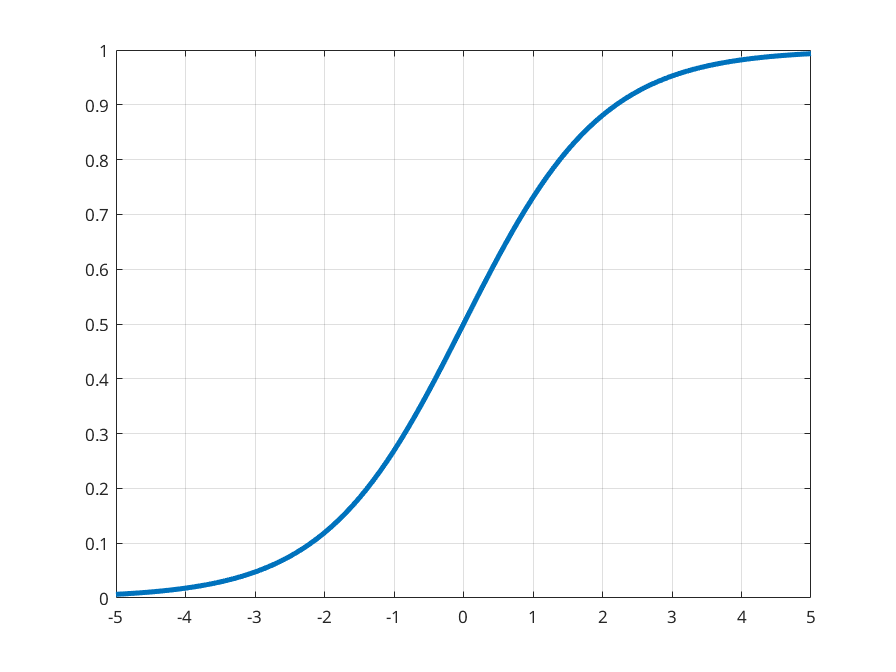
\includegraphics[keepaspectratio,width=8cm]{kep/sigmoid.png}
			\caption{Sigmoid activation function.}
			\label{fig:sigmoid}
		\end{center}
		\end{figure}
		\item \textbf{Hyperbolic tangent (Tanh)} = The output of the tanh function is similar to the sigmoid function, but it ranges between -1 and 1. While the vanishing gradient problem can still occur in very deep neural networks, being centered around 0 helps improve the training process. This centering allows weight adjustments to move faster in the right direction, speeding up convergence. The function is defined as $g(x) = \frac{e^x - e^{-x}}{e^x + e^{-x}}$ and its shape can be seen in Figure \ref{fig:tanh}.
		\begin{figure}[H]
		\begin{center}
			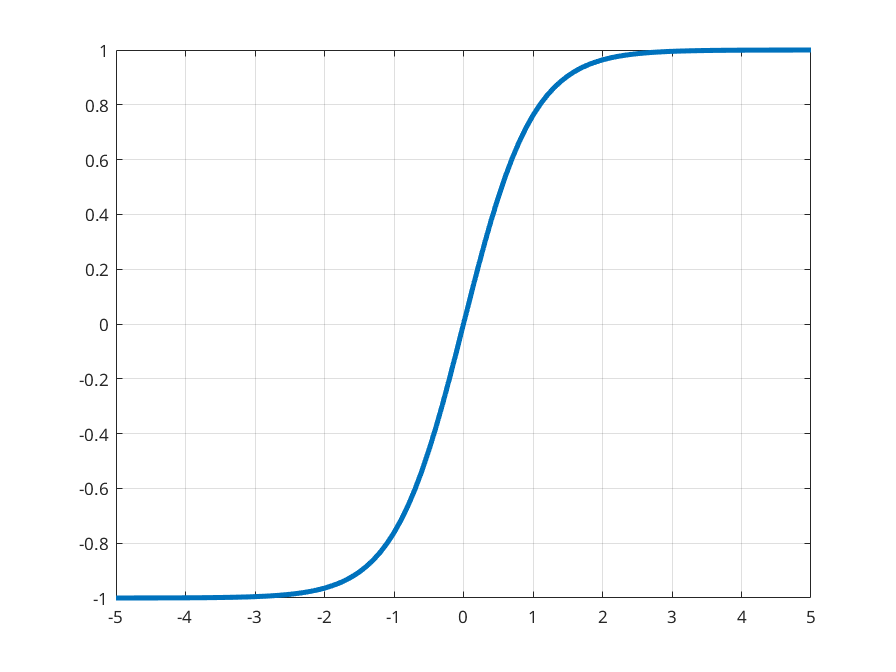
\includegraphics[keepaspectratio,width=8cm]{kep/tanh.png}
			\caption{Hyperbolic tangent activation function.}
			\label{fig:tanh}
		\end{center}
		\end{figure}
		\item \textbf{Rectified linear unit (ReLU)} = A very simple function that outputs only positive values, with a range of $[0, \infty)$. It's mathematically less expensive than the sigmoid or tanh functions and doesn't suffer from the vanishing gradient problem. The function defined as: $g(x) = max(x, 0)$ and its shape can be seen in Figure \ref{fig:relu}.
		\begin{figure}[H]
		\begin{center}
			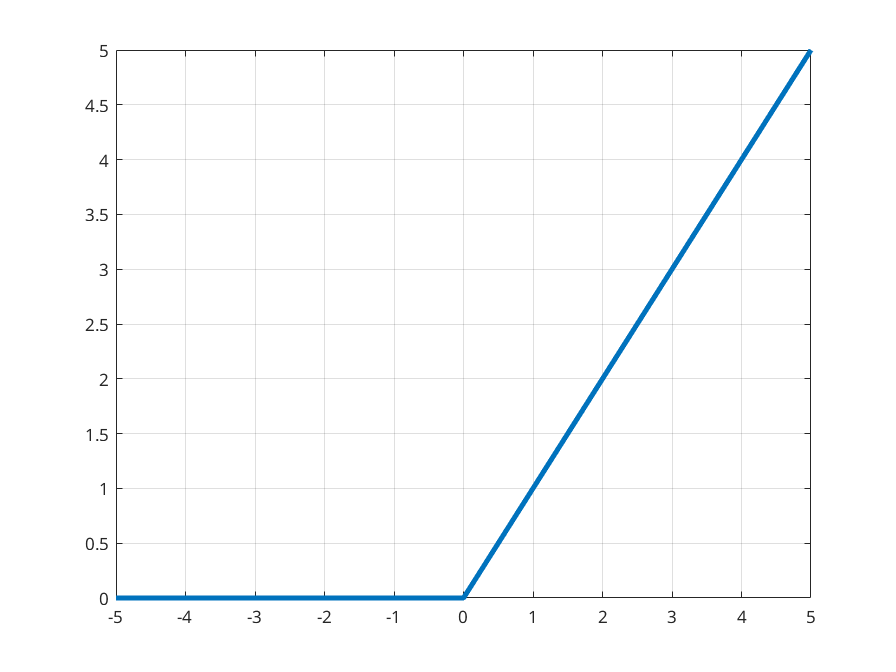
\includegraphics[keepaspectratio,width=8cm]{kep/relu.png}
			\caption{Rectified linear unit activation function.}
			\label{fig:relu}
		\end{center}
		\end{figure}
		\item \textbf{Softmax} = It transforms the final output value of the network into probabilities, ranging between 0 and 1, while ensuring that the sum of all probability values is 1. This function guarantees that each possible class is assigned a probability, making it ideal for multi-class classification problems. The shape of the function can be seen in Figure \ref{fig:softmax}.
		\begin{figure}[H]
		\begin{center}
			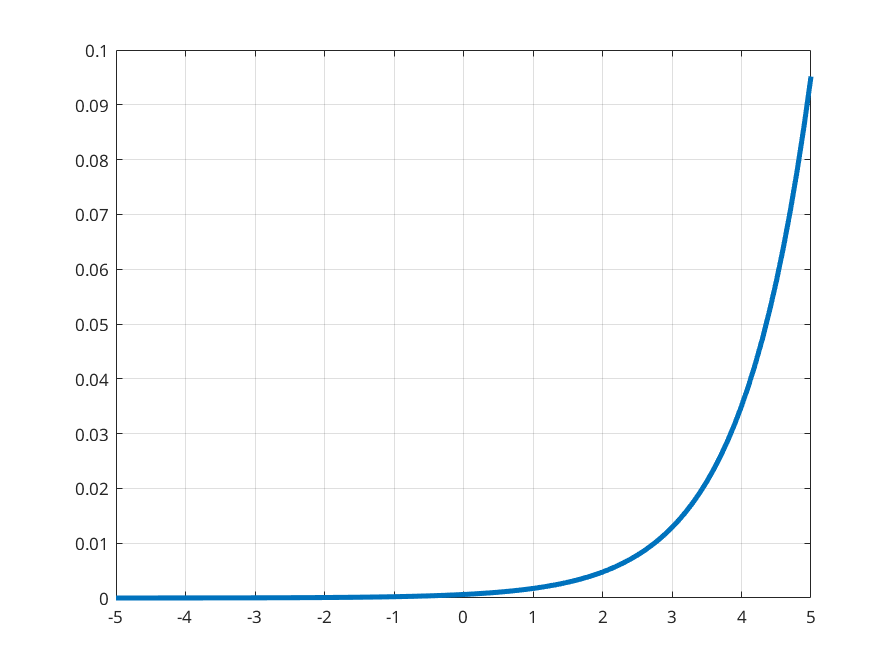
\includegraphics[keepaspectratio,width=8cm]{kep/softmax.png}
			\caption{Softmax activation function.}
			\label{fig:softmax}
		\end{center}
		\end{figure}
	\end{itemize}

	The way neurons are structured and connected primarily determines how the network learns and functions.

		\subsubsection{Single-Layer Feedforward Network}
		In a layered neural network, neurons are organized in a structured, layer-like form. A single-layer neural network is the simplest form of a layered network, where neurons in the input layer are connected to neurons in the output layer. These connections work only in one direction, hence the name feedforward. Since only the output layer performs actual computations, the input layer merely passes information forward, only the output layer is counted, hence the name single-layer neural network. The output signals of the neurons in the output layer is the overall response of the network to the data supplied in the input layer~\cite{NNACF}.
		
		The structure of a single-layer feedforward neural network is presented in Figure~\ref{fig:single-layer feedforward nn}.
		\begin{figure}[H]
		\begin{center}
			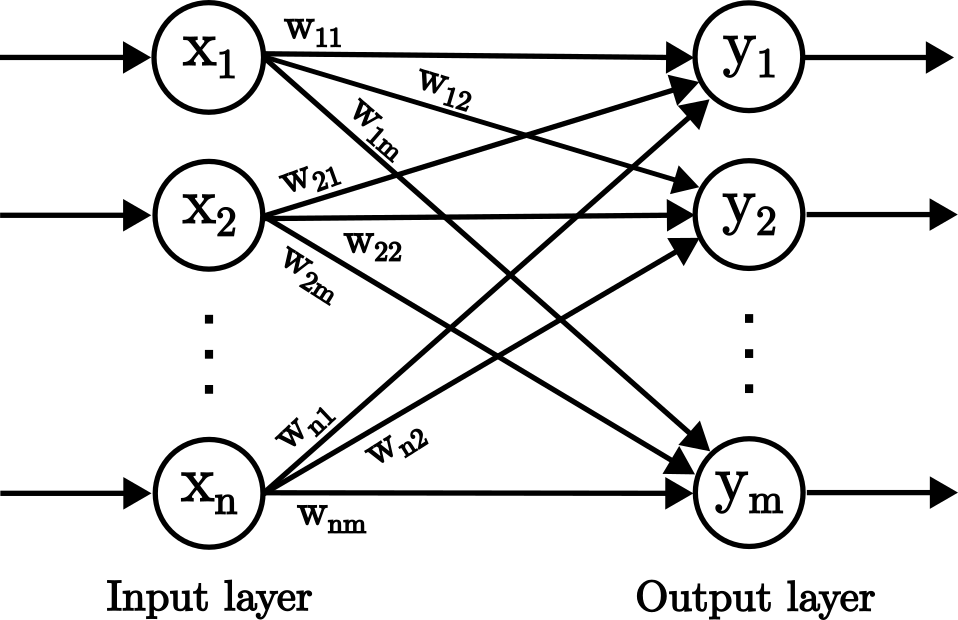
\includegraphics[keepaspectratio,width=10cm]{kep/single_layer_feedforward_nn.png}
			\caption{Single-layer feedforward neural network architecture.}
			\label{fig:single-layer feedforward nn}
		\end{center}
		\end{figure}

		\subsubsection{Multilayer Feedforward Network}
		To effectively solve non-linearly separable problems or extract higher-order statistics, a multilayer feedforward network is recommended. These networks include one or more \textit{hidden layers}, which are positioned between the input and output layers. Hidden layers consist of neurons, referred to as \textit{hidden neurons}, that receive inputs from the output signals of neurons in the preceding layer. The hidden layers enable the network to learn complex representations by applying additional transformations through an extra set of synaptic weights. 

		In Figure \ref{fig:smultilayer feedforward nn}, a fully connected multilayer feedforward neural network is shown. The network is considered \textit{fully connected}, because every neuron in each layer is connected to every neuron in the subsequent layer. If some connections were missing, the network would be considered \textit{partially connected}~\cite{NNACF}.
		\begin{figure}[H]
		\begin{center}
			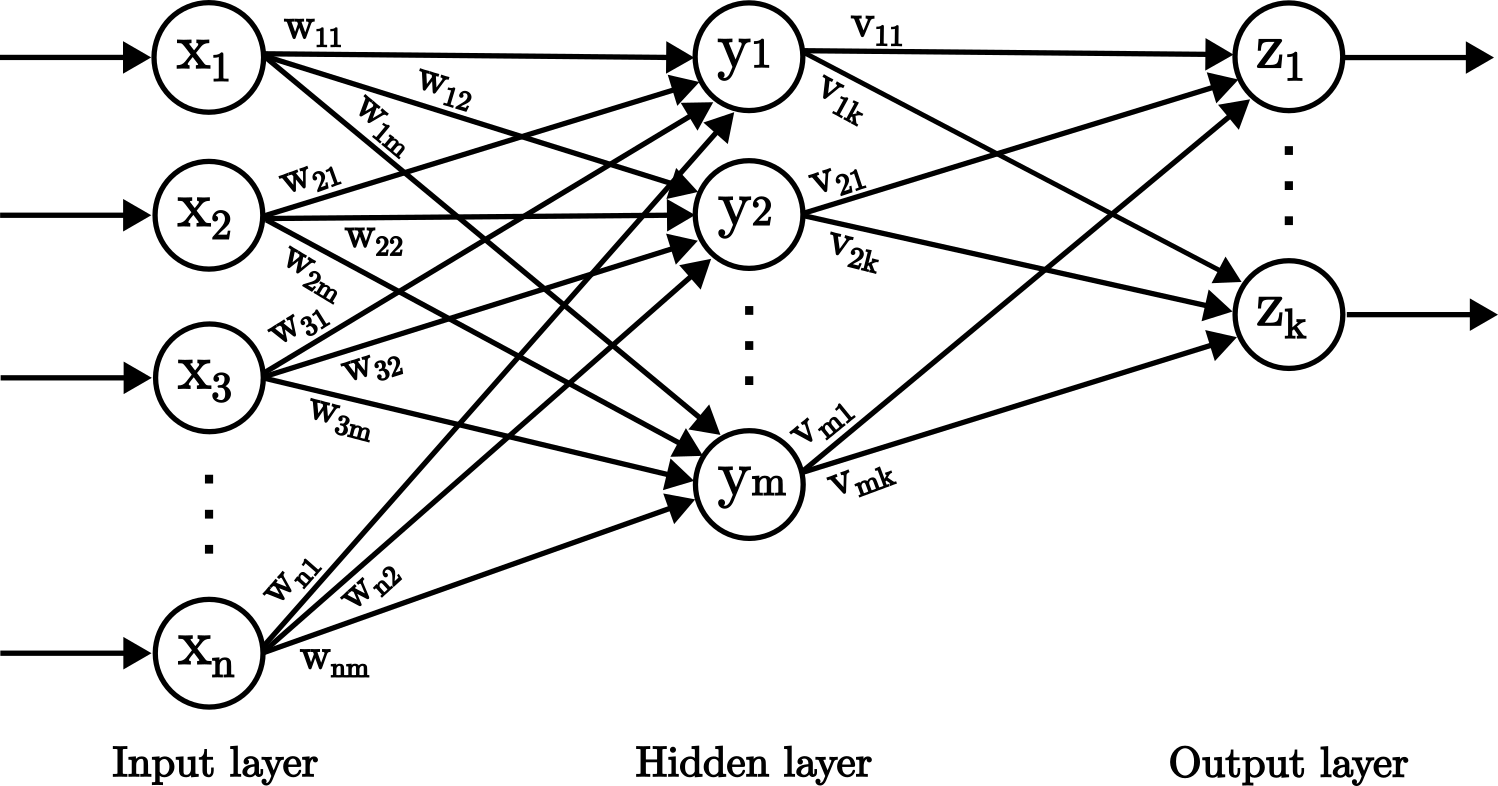
\includegraphics[keepaspectratio,width=14cm]{kep/multi_layer_feedforward_nn.png}
			\caption{Multilayer feedforward neural network architecture with fully connected neurons.}
			\label{fig:smultilayer feedforward nn}
		\end{center}
		\end{figure}
		
		\subsubsection{Convolutional Network (CNN)}
		Convolutional neural networks (CNNs) are a popular choice for solving image classification problems. CNNs mimic the way humans classify images by focusing on specific features that distinguish each object class. They first identify low-level features (such as contour details and patches of color), then higher-level features (such as parts of limbs or faces). The presence or absence of these details determines the probability of each output class.

		This type of neural network combines two specialized hidden layers: convolution and pooling layers. Convolution layers search for small patterns, while pooling layers downsample these patterns.

		A convolution layer consists of multiple convolution filters, each detecting specific local patterns in an image. These filters highlight regions in the image that resemble their learned patterns rather than relying on predefined ones.

		A pooling layer condenses a large image into a smaller, summarized version. This is typically done using operations like \textit{max pooling}, which usually takes a non-overlapping $2 \times 2$ block of pixels and retains only the maximum value within that block~\cite{AISL}.

		The simplified architecture of a CNN can be seen on Figure \ref{fig:cnn}.
		\begin{figure}[H]
		\begin{center}
			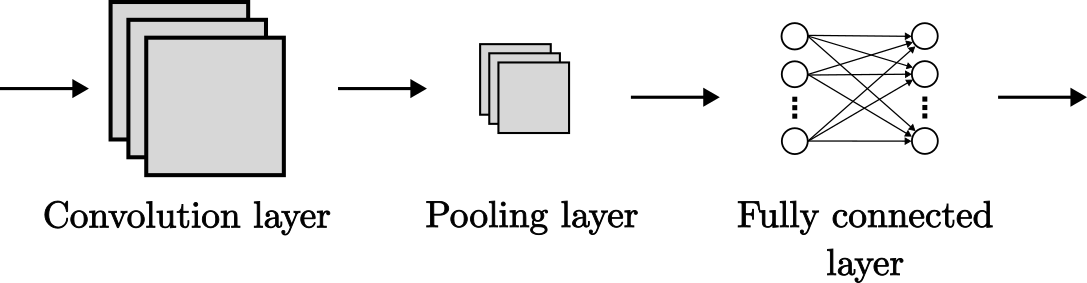
\includegraphics[keepaspectratio,width=14cm]{kep/cnn.png}
			\caption{Convolutional neural network architecture.}
			\label{fig:cnn}
		\end{center}
		\end{figure}
		
		One of the most famous CNN is the LeNet-5 architecture, which became widely used for handwritten digits recognition. The original topology can be seen in Table~\ref{table:lenet_topology}.
		\begin{table}[H]
		\begin{center}
		\begin{tabular}{|c|c|c|c|c|}
		\hline
		\textbf{Layer type} & \textbf{Maps} & \textbf{Size} & \textbf{Kernel size} \\
		\hline
		Fully connected layer & - & 10 & - \\ 
		\hline
		Fully connected layer & - & 84 & - \\ 
		\hline
		Convolution layer & 120 & $1 \times 1$ & $5 \times 5$ \\ 
		\hline
		Average pooling layer & 16 & $5 \times 5$ & $2 \times 2$ \\
		\hline
		Convolution layer & 16 & $10 \times 10$ & $5 \times 5$ \\
		\hline
		Average pooling layer & 6 & $28 \times 28$ & $5 \times 5$ \\
		\hline
		Image input layer & 1 & $32 \times 32$ & - \\
		\hline
		\end{tabular}
		\end{center}
		\caption{Topology of LeNet-5.}
		\label{table:lenet_topology}
		\end{table}
		
		The first row of Table~\ref{table:lenet_topology} holds the output layer with neurons for each possible digit and the last row holds the input layer designed for images with a size of $32 \times 32$. The \textit{maps} column of the table refers to the number of feature maps the given convolution layer produces. A feature map highlights a specific feature of the input image. The \textit{size} column refers to the size of the input to a given convolutional or pooling layer. In the case of the fully connected layers, it refers to the number of neurons. The \textit{kernel size} column shows the size of the convolution filters or in the case of pooling layers, the size of the pooling operation~\cite{HMLSKT}.
		
		Another important property of convolution and pooling layers is \textit{stride}, which determines the size of steps the convolution filter or pooling operation moves across the input image.

		\subsubsection{Recurrent Network (RNN)}
		A recurrent neural network (RNN) is another type of multilayer neural network, but it differs from feedforward networks in that it has at least one feedback loop. The structure of a simple RNN is shown in Figure \ref{fig:rnn}. This structure includes self-feedback loops, where the output of a neuron is fed back into its input. In this setup, neurons $x_1$ and $x_3$ are hidden neurons, each with a unit-delay element before its input. These units store and pass the previous hidden state to the next time step, allowing the network to retain temporal dependencies~\cite{NNACF}.
		\begin{figure}[H]
		\begin{center}
			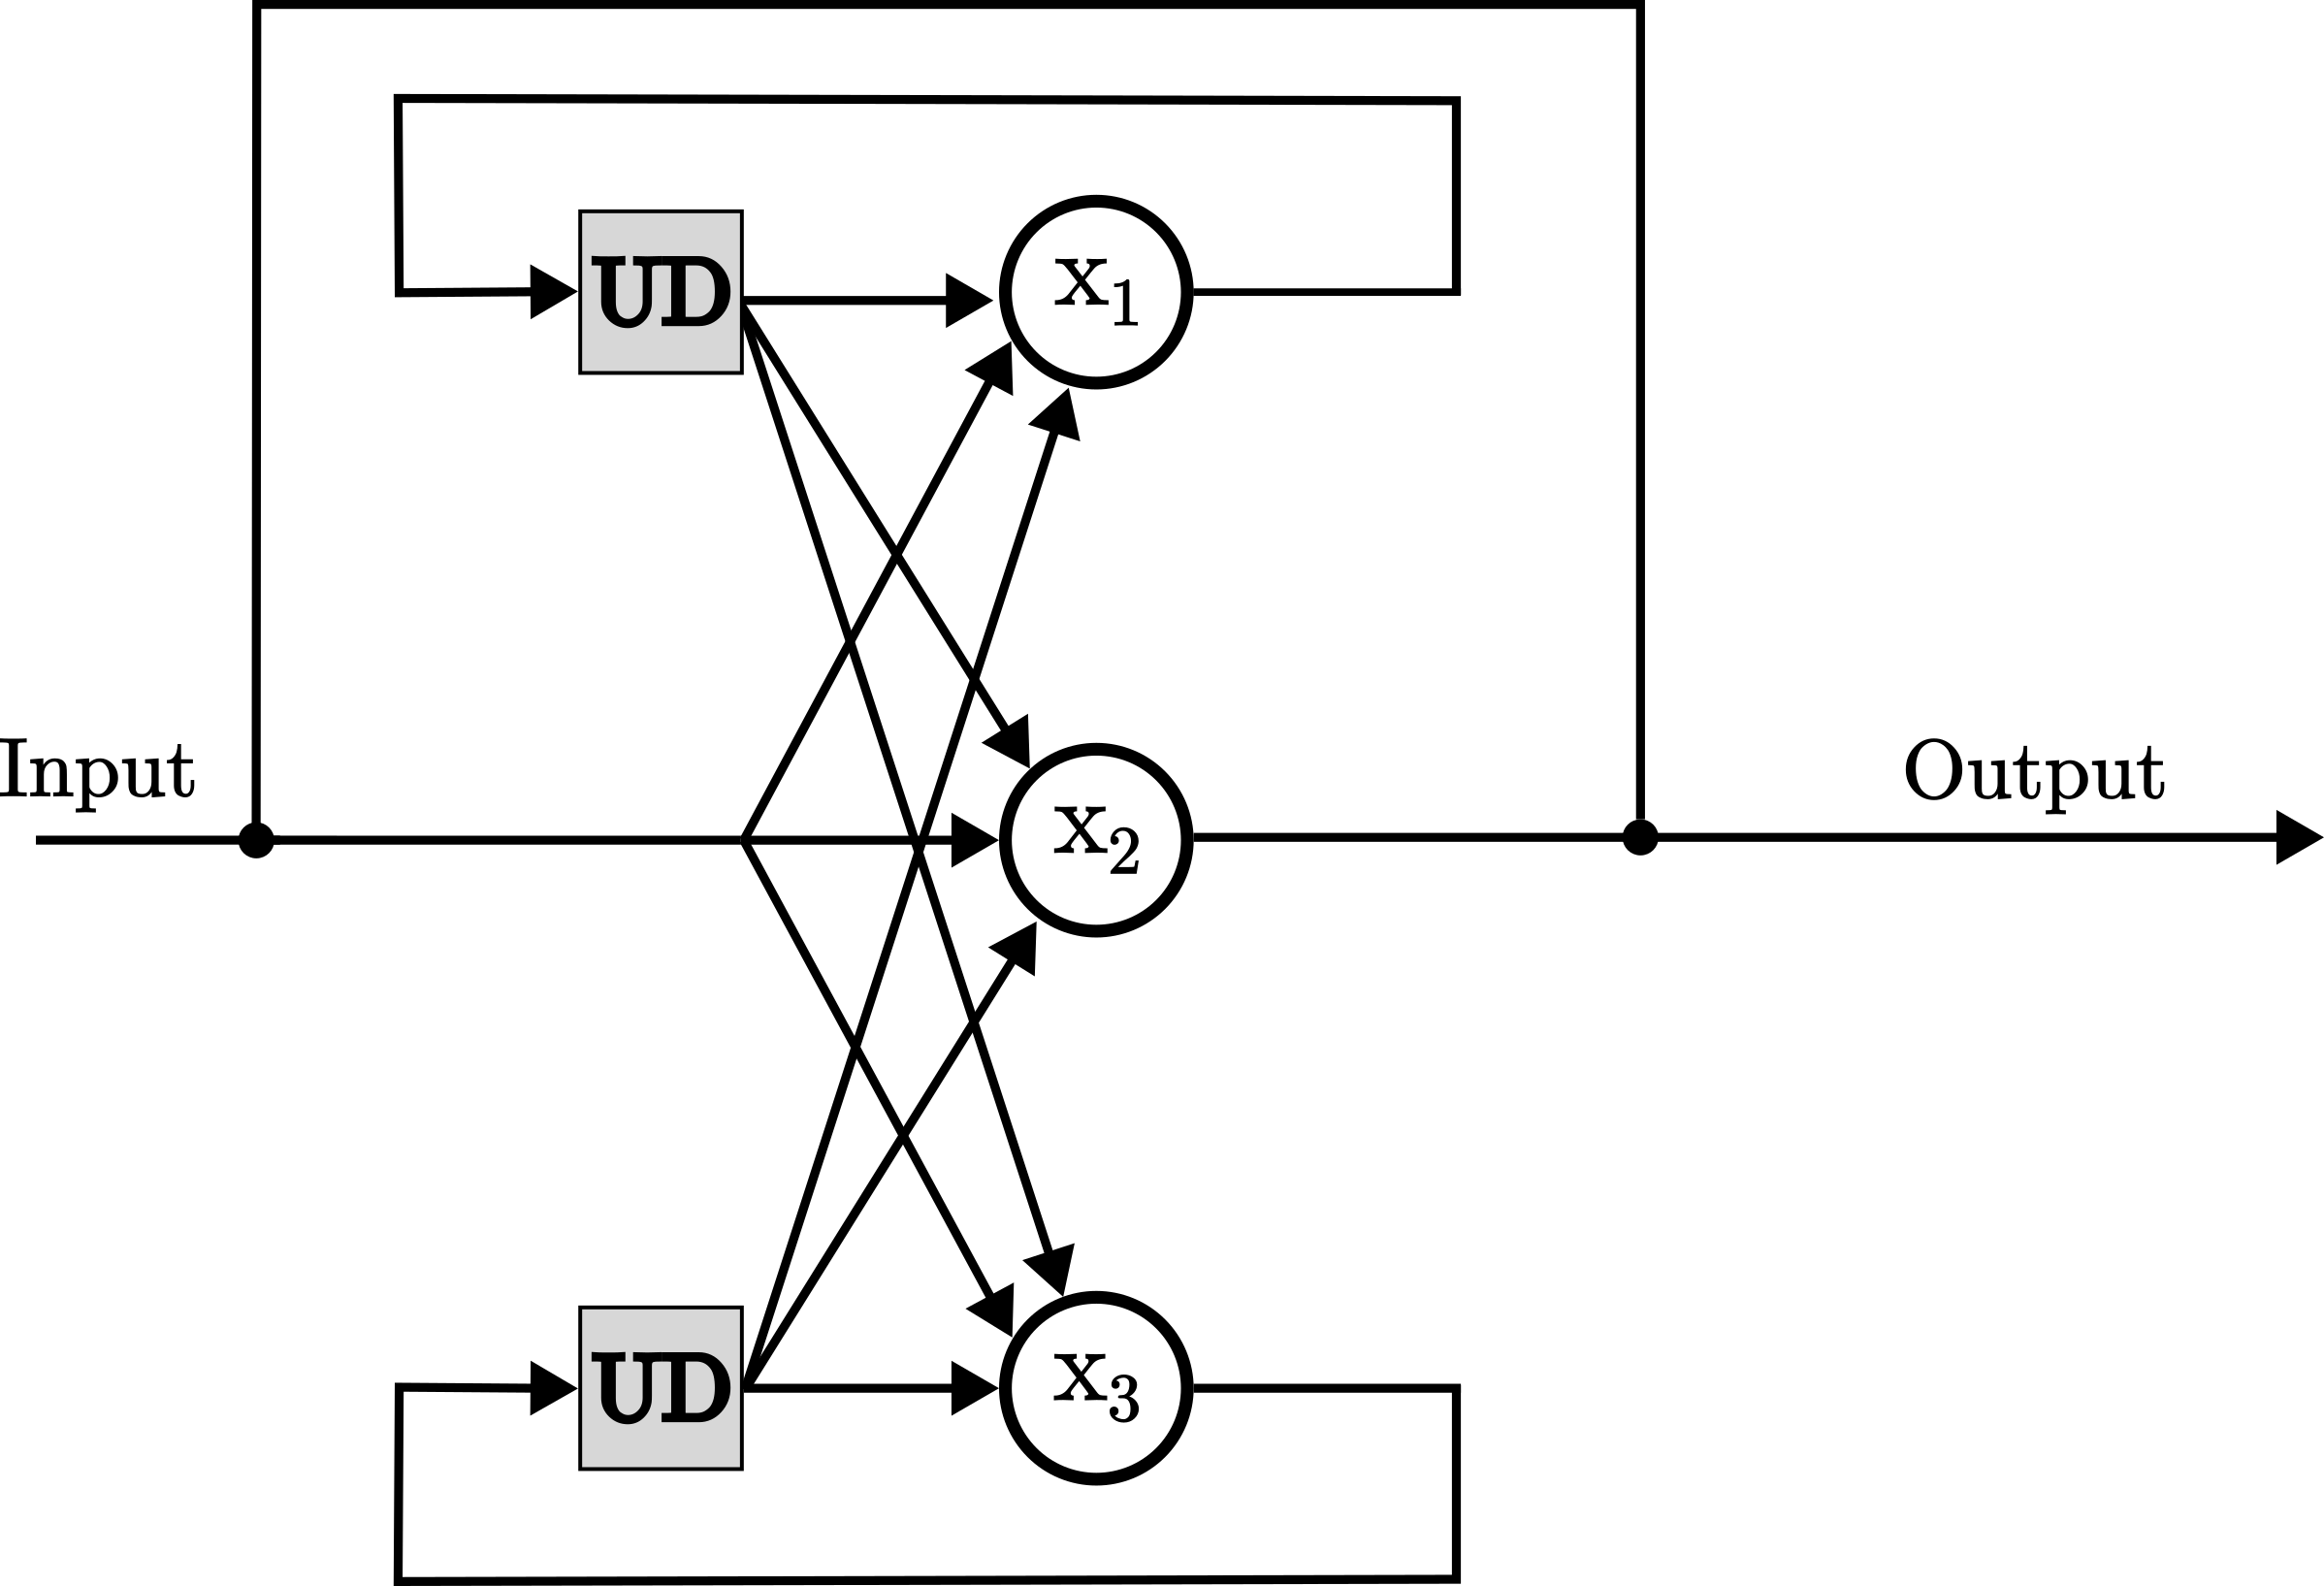
\includegraphics[keepaspectratio,width=10cm]{kep/rnn.png}
			\caption{Recurrent neural network architecture.}
			\label{fig:rnn}
		\end{center}
		\end{figure}
		The input to an RNN is a sequence. For example, a document can be organized as a sequence of words. The order of the words and the frequent pairing of words in a sentence carry semantic meaning. An RNN can take advantage of the sequential nature of such inputs, much like convolutional neural networks leverage the spatial structures of objects in images. The output of an RNN can either be a sequence (as in text translation) or a scalar (as in classification problems)~\cite{AISL}.

		When handling sequences, RNN store past information through loops and a \textit{hidden state}. This hidden state acts as memory, retaining information from previous time steps to help the network maintain context and process sequential data effectively. RNNs have two sets of weights: one for the input and one for the hidden state. These weights are both updated during the training process. The output of an RNN depends on the current input and the hidden state, which is influenced by previous inputs~\cite{HLSTMW}.

		However, simple RNNs suffer from the \textit{vanishing gradient problem}. The vanishing gradient problem occurs when the gradients of the loss function, with respect to the model's weights, become very small in deep neural networks, making it difficult for the model to learn. In this context, a gradient indicates how much the model's output changes when the weights are adjusted during learning and the loss function measures how far the model's prediction is from the correct answer. This problem occurs, because the gradients shrink as they are propagated backward through the layerss during training~\cite{VGPCCS}.

		The vanishing gradient problem is alleviated by Long Short-Term Memory (LSTM) networks. LSTM is a type of RNN specifically designed to prevent the network's output from decaying or exploding as it cycles through feedback loops, enabling it to learn long-term dependencies~\cite{LSTM}.

		In addition to the hidden state in traditional RNNs, an LSTM unit includes a memory cell, an input gate, an output gate, and a forget gate. The hidden state functions as in a standard RNN, carrying information from previous time steps to influence the current output. The memory cell stores long-term information, acting as the unit's memory. Each gate has its own weights and biases. The input gate controls what new information is added to the memory cell. The output gate determines how much of the stored information is used to compute the LSTM block’s output. Finally, the forget gate decides which past information should be discarded from the memory cell~\cite{HLSTMW}.
		
		The structure of an LSTM unit can be seen on Figure \ref{fig:lstm}.
		\begin{figure}[H]
		\begin{center}
			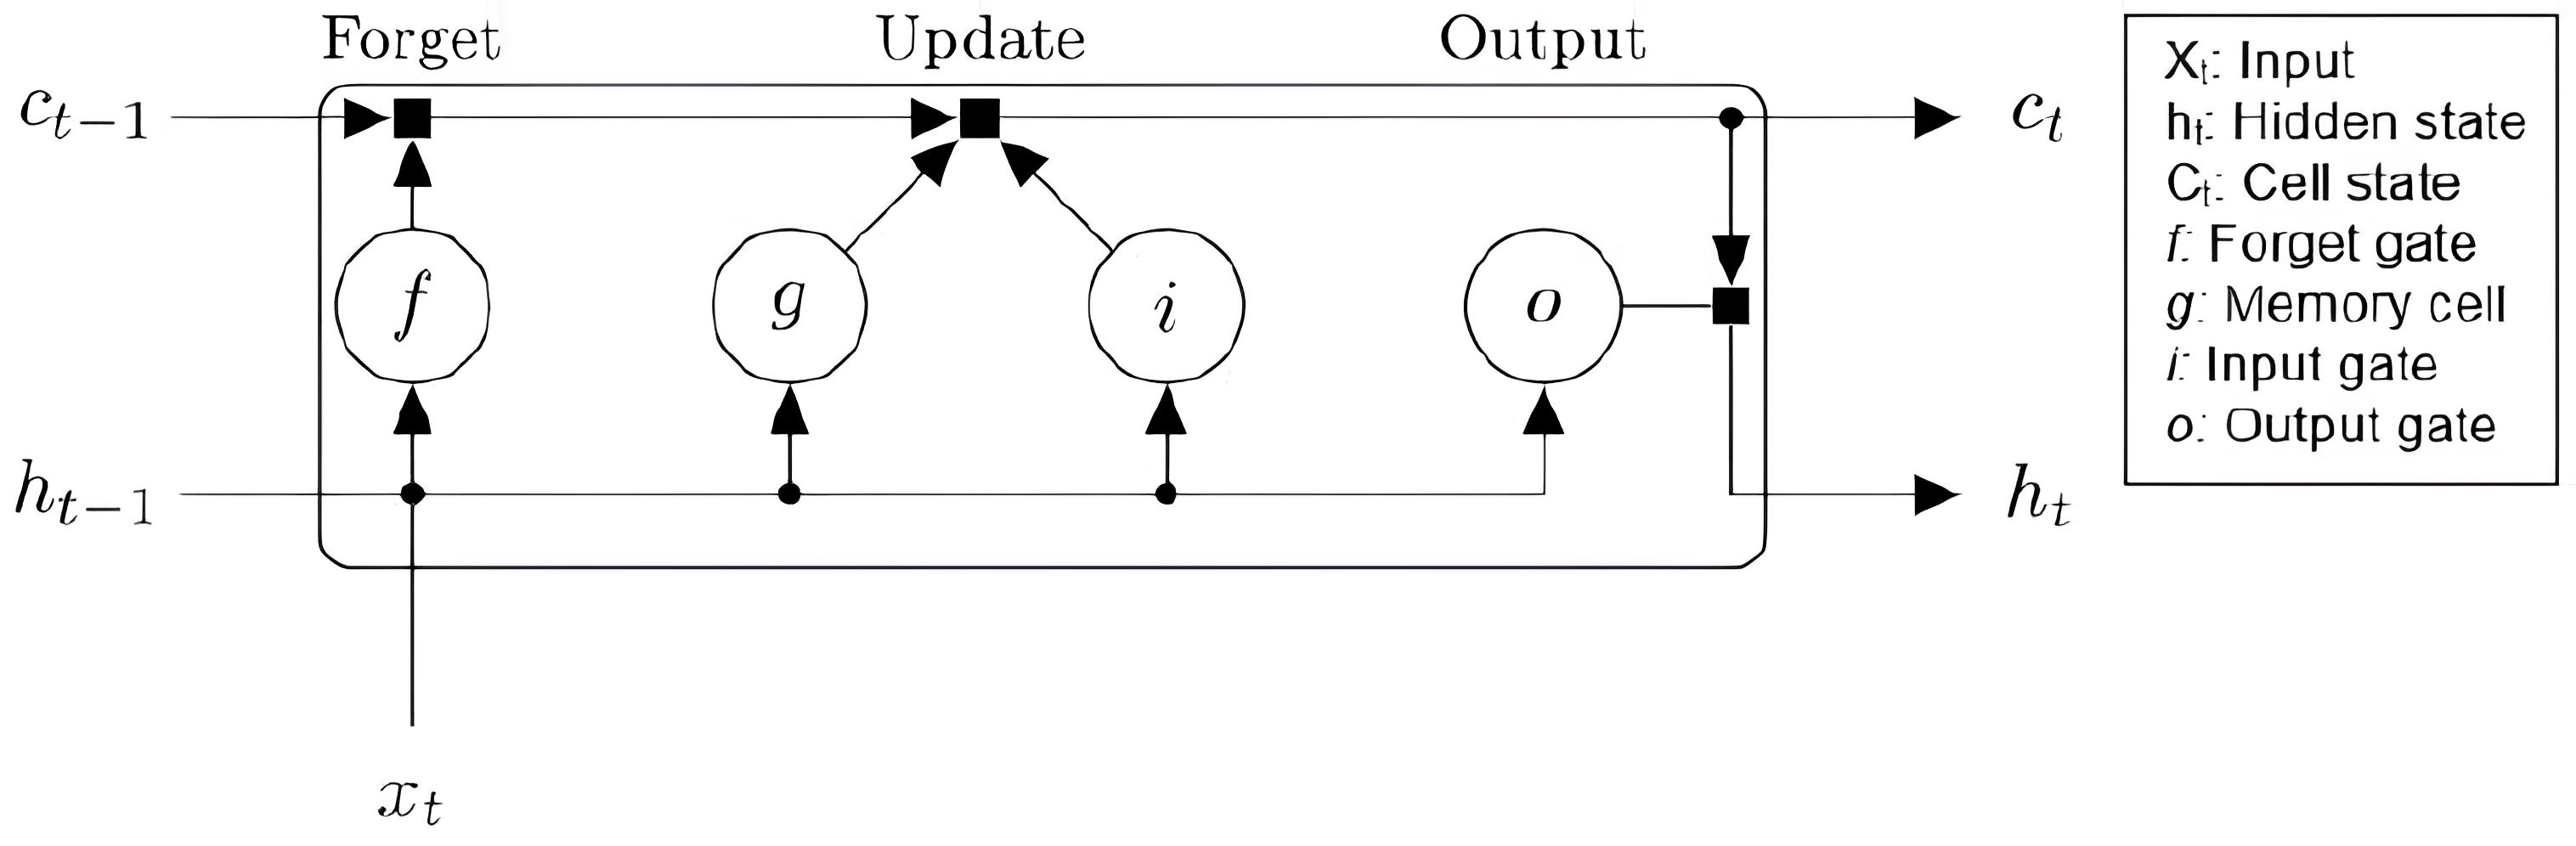
\includegraphics[keepaspectratio,width=14cm]{kep/lstm.jpg}
			\caption{Long Short-Term Memory architecture~\cite{HLSTMW}.}
			\label{fig:lstm}
		\end{center}
		\end{figure}
		Due to their ability to learn long-term dependencies, LSTMs are suitable for a variety of sequence learning tasks, including language modeling and translation, acoustic modeling of speech, speech synthesis, speech recognition, handwriting recognition, all other kind of time series prediction and more~\cite{LSTM}.

	\subsection{Types of Learning}
	Generally, machine learning systems can be grouped based on the type and amount of supervision received during the training. The most common types of learning are:
	\begin{itemize}
		\item Supervised learning
		\item Reinforcement learning
		\item Unsupervised learning~\cite{HMLSKT}
	\end{itemize}
		
		\subsubsection{Supervised Learning}
		For supervised learning a training set is available. The training set consists of numerous observations with predefined inputs and a corresponding output. The inputs are called predictors (also called features) and the output is referred to as the response. The observations represents individual data instances~\cite{TESL}.

		For each predictor measurement vector $x_i$ (where $i = 1, ..., n$), there is a corresponding response measurement $y_i$. The goal of learning is to fit a model that links the response to the predictors, either to predict the response for future observations or to gain a deeper understanding of the relationship between the response and the predictors~\cite{AISL}.

		As an example, lets say we want to predict house prices and we have the following training set:
		\begin{table}[H]
		\begin{center}
		\begin{tabular}{|c|c|c|c||c|}
			\hline
			\textbf{Housing type} & \textbf{Size ($m^2$)} & \textbf{Number of rooms} & \textbf{Location} & \textbf{Price (€)}\\
			\hline
			Single-family home & 250 & 4 & Bratislava & 412000\\
			\hline
			Single-family home & 390 & 6 & Komárno & 186000\\ 
			\hline
			Apartment & 55 & 2 & Trnava & 118900\\
			\hline
			Single-family home & 180 & 4 & Košice & 375000\\
			\hline
			\multicolumn{5}{|c|}{$\cdots$} \\
			\hline
		\end{tabular}
		\end{center}
		\caption{Example training set with arbitrary values.}
		\label{table:example_train_set}
		\end{table}
		In Table~\ref{table:example_train_set} each row corresponds to a single house for sale. These houses are the observations and each column (excluding the last column) of the table, which represents the attributes of the houses, is an input, or a predictor. The last column is the output or the response.

		The variables (be that predictor or response) can be described as either quantitative or qualitative. Quantitative variables are numerical values, like the size, number of rooms and price of a house in Table~\ref{table:example_train_set}. Qualitative variables take values in one of $K$ different categories, like the type of housing in Table~\ref{table:example_train_set}. 
		
		Problems with a quantitative response are referred to as regression problems, while problems with a qualitative response are referred to as classification problems~\cite{AISL}.

		\subsubsection{Reinforcement Learning}
		In reinforcement learning, a virtual object called an agent can make observation of its environment, commit actions resulting in rewards or penalties (usually defined as negative rewards) based on the outcome. An episode is a complete sequence of these interactions, starting from an initial state and continuing until the agent reaches a terminal state or a stopping condition. During an episode, the agent learns by receiving feedback (the rewards), which guides it to improve its actions over time~\cite{HMLSKT}.

		In reinforcement learning, the goal is to figure out a strategy (called a policy) that tells the agent what actions to take in different situations, in order to get the most reward over time. The policy can either be deterministic, where the the agent always picks the same action for a given situation, or stochastic, where the action is chosen probabilistically. The agent needs to learn how actions and rewards are connected, which means it needs to explore the policy space through trial and error. Policy space refers to the set of all possible policies that an agent can adopt~\cite{RLRAS}.

		More precisely, this policy could be a neural network, which takes observations as inputs and outputs the resulting action. Alternatively, the policy could be a genetic algorithm, where each generation consists of multiple policies and new generations of policy offsprings are created based on the genetic algorithm used. Reinforcement learning is commonly used in robotics and smart home appliances. We can also find financial securities trading support systems using reinforcement learning~\cite{HMLSKT}.

		\subsubsection{Unsupervised Learning}
		If we only have a set of unlabeled measurement vectors $x_i$ (where $i = 1, ..., n$) with no corresponding $y_i$ response, we talk about unsupervised learning. Since we don't have an associated response, the goal of unsupervised learning is not to make predictions, but rather to analyze and discover patterns in the available data, which makes often makes working with unsupervised learning algorithms subjective. Furthermore, the lack of a corresponding response makes evaluating the obtained results difficult, as there is no way to check our work without knowing the true answer. This method of learning is often used as part of an exploratory data analysis. For example, a researcher might analyze gene expression levels in patients with certain health conditions to identify relationships or subgroups among the genes. A webstore could perform sales analyses to identify groups of customers with similar purchase histories for targeted advertisements and service customization. Similarly, a search engine might customize search results for users based on the click histories of other users with similar search patterns~\cite{AISL}.

		For applications like these, where groups of objects or persons are identified, clustering algorithms are used. Another frequently used method in unsupervised learning is data visualization, which transforms complex, unlabeled data into a format suitable for plotting or further analysis. A related task is dimensionality reduction, where the aim is to simplify data with minimal information loss by performing feature extraction and merging correlated features. Anomaly detection algorithms can be used to detect fraudulent actions or to remove outliers from datasets during preprocessing~\cite{HMLSKT}.


	\subsection{Learning Parameters}
	During the training process there are numerous variable parameters that need to be tailored depending on the model's objective.
		\subsubsection{Epoch}
		An \textit{epoch} refers to one pass through the entire training set. Setting this value too low causes the training process to stop early and the model to not capture the underlying patterns in the data, leading to poor performance. This is called \textit{underfitting}. Setting the value too high can increase the training time and cause the model to fit too closely to the training data, making it unable to generalize for real-life use. This is called \textit{overfitting}~\cite{WIEML}.

		The number of epochs doesn't have to be set to an exact value. Often, it's set to a large number, and training is stopped early based on the model's performance during training to prevent overfitting and save time.

		\subsubsection{Learning Rate}
		The \textit{learning rate} (often denoted as $\alpha$) in machine learning controls the magnitude of weight updates applied by the chosen optimization method during training epochs, affecting training speed, stability, and performance. Finding the optimal value is crucial, especially for deep neural networks. Setting a value too low can make the training slow and ineffective by getting stuck in a local minimum, while setting the rate too high can cause overstepping of the optimal state, making the model fail to converge~\cite{MML}.

		A \textit{fixed learning rate} means that a constant learning rate is selected and maintained throughout the training process. This is a simple approach, but it may be slow and may not converge effectively in complex training scenarios.

		Using \textit{learning rate schedules}, the learning rate can be adjusted based on a predefined schedule. The rate can be decreased after a fixed number of steps or by defining function based decay, e.g., \textit{Exponential decay}, where the decay decreases exponentially over time. This method can enhance convergence and learning performance, while still remaining relatively simple. 

		Another common variant is the \textit{adaptive learning rate}, where the rate can be dynamically adjusted based on the model's performance during the training process. This helps optimize convergence speed and stability, avoiding issues like overshooting minima, but it behaves less predictably and is computationally more expensive~\cite{LRSALRMDL}.

		\subsubsection{Batch Size}
		In batch-based learning, the \textit{batches} are partitions of the training set and the batch size defines the number of samples processed before updating the weights. When the entire training set is used as a single batch, it's called \textit{batch gradient descent}. When each batch consists of a single sample, it's called \textit{stochastic gradient descent}. When the batch size falls between these two extremes, the training is referred to as \textit{mini-batch gradient descent}. If the batch size doesn't divide the training set equally, the final batch will either have fewer samples or will be discarded entirely~\cite{DBBENN}.

		Choosing a small batch size for supervised learning can lead to more frequent weight updates, resulting in slower training and noisy gradients. However, it can also help escape local minima, potentially improving generalization. A smaller batch size also requires less memory, making it ideal for machines with lower hardware specifications. Using a larger batch size can speed up training and provide a more stable learning process with smaller computing costs due to fewer updates. However, it is more prone to getting stuck in local minima and requires more memory~\cite{HDBSIYML}.

		\subsubsection{Loss Function}
		The \textit{loss function} of the network (sometimes referred to as the \textit{objective function} or \textit{cost function}) takes the predictions of the network and the correct answer and computes a distance score, indicating how well the network performed on a given example. The selected optimization method then uses this score to adjust the weights in a direction that lowers the score for the given example~\cite{DLP}.

		For a regression problem, the most commonly used loss function is the \textit{Mean Squared Error} (MSE). The function is defined as:
		\[ MSE = \frac{1}{n} \sum_{i=1}^{n} (y_i - \hat{y}_i)^2 \]
		where $y_i$ represents the actual values, $\hat{y}_i$ represents the predicted values and $n$ is the number of samples. The closer the predictions are to the actual values, the smaller the MSE, while larger differences are penalized more~\cite{AISL}.

		In a classification setting, $y_i$ is no longer quantitative but qualitative. One of the most commonly used loss functions in this scenario is the \textit{cross-entropy} function, which measures the difference between the actual and predicted probability distributions. In the training set, the probability of an example belonging to a specific class is either 1 or 0. The classes are usually \textit{one-hot encoded}, meaning that if a sample belongs to class 2 out of five possible classes, it's represented as [0 1 0 0 0].

		The function for a single sample is defined as:
		\[ L = -\sum_{k=1}^{n} y_k log(\hat{y_k}) \]
		where $y_k$ is the actual probability of class $k$, $\hat{y}_k$ is the predicted probability of class $k$ and $n$ is the number of classes. The more probability the model assigns to the correct class, so the more confident it is, the lower the loss and vice versa~\cite{AISL}.

		The function encourages confidence in correct predictions, penalizes large errors more heavily and penalizes uncertainty less than confident incorrect predictions~\cite{BOCEL}.

		\subsubsection{Optimization Method}
		The objective of the selected optimization method is to adjust the model's parameters (e.g. the synaptic weights) to achieve the lowest value of the loss function. Each optimization technique fine-tunes the model differently and is chosen based on the specific goal to be achieved~\cite{COOTMLT}. The various variants of the \textit{gradient descent} algorithm are among the most commonly used optimization methods.

		Gradient descent minimizes a function by iteratively moving in the direction of the steepest descent (the negative gradient). It updates parameters using:
		\[ \Theta_{i+1} = \Theta_{i} - \gamma(\nabla f(\Theta_i)) \]
		where $\Theta_{i}$ and $\Theta_{i+1}$ are the current and next points respectively (in our case, the current and next values of a parameter like a weight), $\gamma$ is the step size (in our case the learning rate) and $\nabla f(\Theta_i)$ is the gradient of the (loss) function $f$ at $\Theta_i$.

		One common variant of the gradient descent algorithm is \textit{stochastic gradient descent} (SGD). Instead of computing the exact gradient over the entire dataset, which can be time consuming, SGD approximates it by using individual samples~\cite{MML}.

		A key feature of SGD is that, unlike standard (batch) gradient descent, which uses the entire dataset for each update, it performs updates more frequently, making it computationally more efficient and enabling faster convergence in practice~\cite{COOTMLT}.

		SGD can be defined as:
		\[ \Theta_{i+1} = \Theta_{i} - \gamma (\nabla f(\Theta_i, x^j, y^j)) \]
		where $(x^j, y^j)$ represents a single sample from the dataset~\cite{SGD}.

		The SGD algorithm has many derivatives. One increasingly common variant is called the Adam optimizer. The Adam optimizer is an adaptive learning rate optimization algorithm. It combines the advantages of two other extensions of SGD: \textit{Momentum} and \textit{RMSProp}. It adjusts the learning rate for each parameter individually, using estimates of the first and second moments of the gradients. Adam is computationally more efficient than its competitors in most cases and is well-suited for large datasets~\cite{AO}.

\section{Machine Learning for Algorithmic Trading}
	Numerous trends, including the rise of electronic trading, advancements in computing power, increased data generation and management, and the development of statistical methods, have driven the growth of algorithmic trading and machine learning in economics.

	Tools for automated trading emerged in the early 2000s, initially focused on executing sell orders cost-effectively by breaking them into smaller chunks to minimize market impact. Later alternative tools for the buy side were developed, enabling the creation of buy orders based on transaction costs, liquidity, and short-term price and volume forecasts.

	ML now also plays a key role in high-frequency trading (HFT), where automated trades are executed with minimal latency and assets are held for very short periods. The goal of HFT is to exploit market inefficiencies. Since many ML algorithms excel at identifying patterns in large datasets, they help HFT traders predict price movements, detect arbitrage opportunities and optimize trading strategies.

	In recent years some hedge funds have moved towards true machine learning, where AI systems analyze large amounts of data, learn from it and assist in decision-making. Hedge funds such as Rebellion Research, Sentient and Aidyia have relied on evolutionary algorithms and deep learning to create fully automatic investment platforms.

	Historically, hedge funds have also relied on alternative data sources before making investment decisions, such as surveys of shoppers or voters ahead of elections or referendums. Since then, the use of alternative data has expanded significantly, and the most sophisticated systems now rely on sources such as satellite images and geolocation data from mobile phones, which can indicate how many people are visiting stores. It's also possible to gain insights into a company's health by tracking the decline in job listings on its website or by scraping data from various websites. Additionally, conclusions can be drawn from employee reviews of their workplaces, customer reviews of products and even from declining prices of products. These alternative data sources are often combined with advanced ML algorithms to help create predictive models that enhance trading strategies and to gain edge over competitors~\cite{MLAT}.

	In this thesis, we will not explore alternative data sources, but instead will rely on more conventional data, such as various information derived directly from the stock market. This section describes three executions of ML models designed to assist in making trade decisions.

	\subsection{Stock Trading Bot Using Deep Q-Learning~\cite{STBDQ}}
	A good example of a common approach in algorithmic trading can be illustrated by the "Stock Trading Bot using Deep Q-Learning" project created by Prabhsimran Singh. This project demonstrates an automatic stock trading bot using Deep Q-Learning, a type of reinforcement learning algorithm utilizing a deep neural network to approximate the optimal action-value function (also known as Q-function), which determines the best action to take in a given state~\cite{HCTDRL}.

	At any moment, the agent observes its current state (an $n$-day window of closing stock prices), selects and performs a trading action. The next state is evaluated and the agent receives a reward accordingly. There is no reward for the \textit{hold} action, and there is no immediate reward for the \textit{buy} action. When the agent makes a \textit{sell} action, the reward is calculated based on the difference between the current price and the bought price. This reflects the quality of both the \textit{buy} and \textit{sell} actions.

	The agent then updates its parameters by minimizing the computed loss. In reinforcement learning loss refers to the differnece between the target Q-value and the predicted Q-value, with the Q-value defining the optimal state-action (quality) values~\cite{HMLSKT}.

	Since the project is open-source and published under the MIT license, anyone can analyze and run the code. The pretrained models included in the repository were trained on Google stock using historical data from 2010. For personal testing, the provided historical Google stock data from 2019 was used.

	The simulation starts with a portfolio worth \$1050 in January. By late December, the portfolio's value increased to \$1359.34, generating a gross profit of \$309.34. This is a gross profit because the simulation does not account for fees required to execute the trades. The evolution of the portfolio's value is visualized using a script included in the repository.

	Looking at Figure \ref{fig:STBRL portfolio evolution}, we can see that the algorithm tends to sell when the price increases and buy when the price decreases.
	\begin{figure}[H]
	\begin{center}
		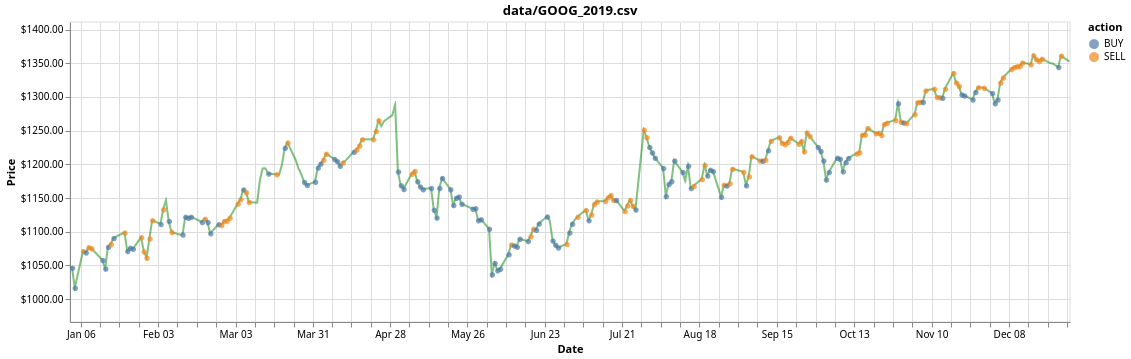
\includegraphics[width=\linewidth]{kep/trade_bot_visualization.png}
		\caption{The evolution of portfolio value using a pretrained trading bot.}
		\label{fig:STBRL portfolio evolution}
	\end{center}
	\end{figure}

	\subsection{A Deep Reinforcement Learning Framework for the Financial Portfolio Management Problem~\cite{ADRLFFPMP}}\label{paper_ADRLFFPMP}
	Another example of the use of reinforcement learning in the financial world is presented in the paper of Zhengyao Jiang, Dixing Xu and Jinjun Liang, titled "A Deep Reinforcement Learning Framework for the Financial Portfolio Management Problem". 
	
	The paper describes the development of a system capable of automating portfolio management. Portfolio management is defined as the action of continuous reallocation of a capital into a number of financial assets. The core of the system is the Ensemble of Identical Independent Evaluators (EIIE) topology.  In an EIIE, there are multiple evaluators (models or algorithms), following the same structure or design, but each working independently examining an asset's historical data to predict future growth. The outputs of their individual evaluations are aggregated to make a final decision. The resulting scores from this evaluation are used to determine the portfolio weights for the next trading period. These weights represent the actions the agent will take. If an asset's weight increases, it'll be bought or if it goes down, it'll be sold. The portfolio weights from the last period are fed back into the EIIE for future predictions.

	Three different types of evaluators were tested in this work, a Convolutional Neural Network (CNN), a basic Recurrent Neural Network (RNN) and a Long Short Term Memory (LSTM) architecture. The framework was evaluated on a cryptocurrency exchange market in three different time period (to ensure that the tests cover different market conditions, like fast- or slow-moving market), each lasting 30 minutes. The tests included benchmark strategies, such as Best Stock (selects and invests in a single asset that achieved the highest final adjusted portfolio value over a specified time period), Uniform Buy and Hold (divides the initial capital equally among assets and holds them without rebalancing or trading), Uniform Constant Rebalanced Portfolio (divides the initial capital equally among assets and constantly rebalances on regular interval to ensure that each asset maintains an equal share of the total portfolio value). Additionally, well-known trading strategies, such as ”Follow-the-Winner”, ”Follow-the-Loser”, ”Pattern-Matching”, and ”Meta-Learning” were also tested.

	The input to the neural networks at the end of period $t$ is a tensor, $X_t$, with shape $(f,n,m)$, where $m$ is the number of preselected non-cash assets, $n$ is the number of input periods before $t$ and $f$ is the number of features. The features include the closing price, highest price and lowest price of the chosen asset. The output is a portfolio vector $w_t$, which represents the weights of the different assets and it's based on the input price tensor $X_t$ and the previous portfolio vector $w_{t-1}$. At the beginning of each period, the trading agent reallocates the fund among the assets. The fee for the trading actions is calculated as the maximum possible fee percentage on their chosen trading website, which is 0.25\%. 

	The framework was tested on historical data only with ideal conditions: zero slippage (meaning the trade is executed immediately when an order is placed) and zero market impact (so the value of the trade is too insignificant to influence the market). For the portfolio preallocation the 11 most-volumed assets were selected. For training, historic price data from the past two days were used. The optimal policy was obtained using gradient descent algorithm.

	The agent's environment consists of all available assets in the chosen market. The external part of the environmental state includes the prices of all orders throughout the market's history up to the current moment. Since this information is too large for the agent to process directly, it is sampled through periodic feature extraction. Time is discretized into periods and for each period, the highest, lowest, and closing prices are extracted. The internal part of the environmental state consists of the agent's previous action (the previously mentioned portfolio vector output), defining the environment state at time $t$ as $s_t = (X_t, w_{t-1})$.

	The agent's primary objective is to maximize the final portfolio value at the end of the investment period. The reward function, which the agent tries to maximize, is the average logarithmic cumulative return $R$. This approach measures how well investments grow over time rather than just calculating total profit, allowing for fair performance comparisons between different time lengths. Since rewards are averaged over time, the agent can learn from shorter batches of trading data without concerns about unfair comparisons between long and short trading periods.

	The financial market never stops, so new data keeps coming in indefinitely. Since the agent can't learn from all past data and older prices are less relevant as they have a smaller impact on today's market, the agent uses an \textit{Online Stochastic Batch Learning} (OSBL) method. At the end of each trading period, the latest market data is added to the training set. The agent then randomly select mini-batches to learn from, but recent data is chosen more often, while older data is picked less frequently. The probability of selecting an older mini-batch decreases exponentially, allowing the agent to gradually forget outdated information.

	The time-ranges for the experiments and their corresponding training sets are presented in Figure~\ref{fig:article_tests}.
	\begin{figure}[H]
	\begin{center}
		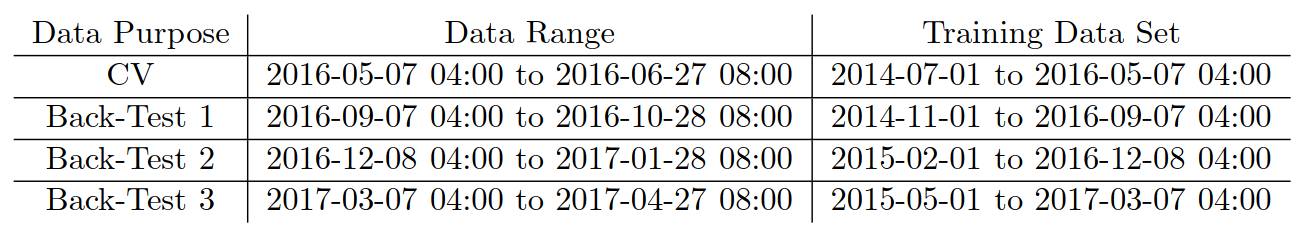
\includegraphics[width=\linewidth]{kep/article_test_ranges.png}
		\caption{Time-ranges of the test and training sets~\cite{ADRLFFPMP}.}
		\label{fig:article_tests}
	\end{center}
	\end{figure}
	Three metrics were used to evaluate the performance of the different approaches. The first metric is the \textit{cumulative portfolio value} ($p_t$) normalized by the initial portfolio value ($p_0$) to adjust for different starting points: $p_t = \frac{p_t}{p_0}$. The second metric is the \textit{Sharpe ratio}, which measures the risk adjusted return of an investment by taking into account the asset's volatility~\cite{SRDFE}. In the experiments, Bitcoin was used as the risk-free asset. Lastly, the third metric is the \textit{Maximum Drawdown}, which highlights downward fluctuations, as the Sharpe ratio treats both upward and downward movements equally. The Maximum Drawdown is defined as the maximum loss from a portfolio's peak to trough over a specific period~\cite{MDDDWFC}.

	After performance evaluation, the CNN-based approach outperformed other trading strategies and benchmarks in the tests. A subset of the results from the second experiment can be seen in Figure~\ref{fig:eiie_results}. Overall, the three variants consistently ranked highest in profitability and risk-adjusted returns, with the only weak point being the Maximum Drawdown. Even under challenging conditions (high transaction costs, frequent trading), the EIIE models remained strong, while traditional strategies and benchmarks often failed or struggled. 
	\begin{figure}[H]
	\begin{center}
		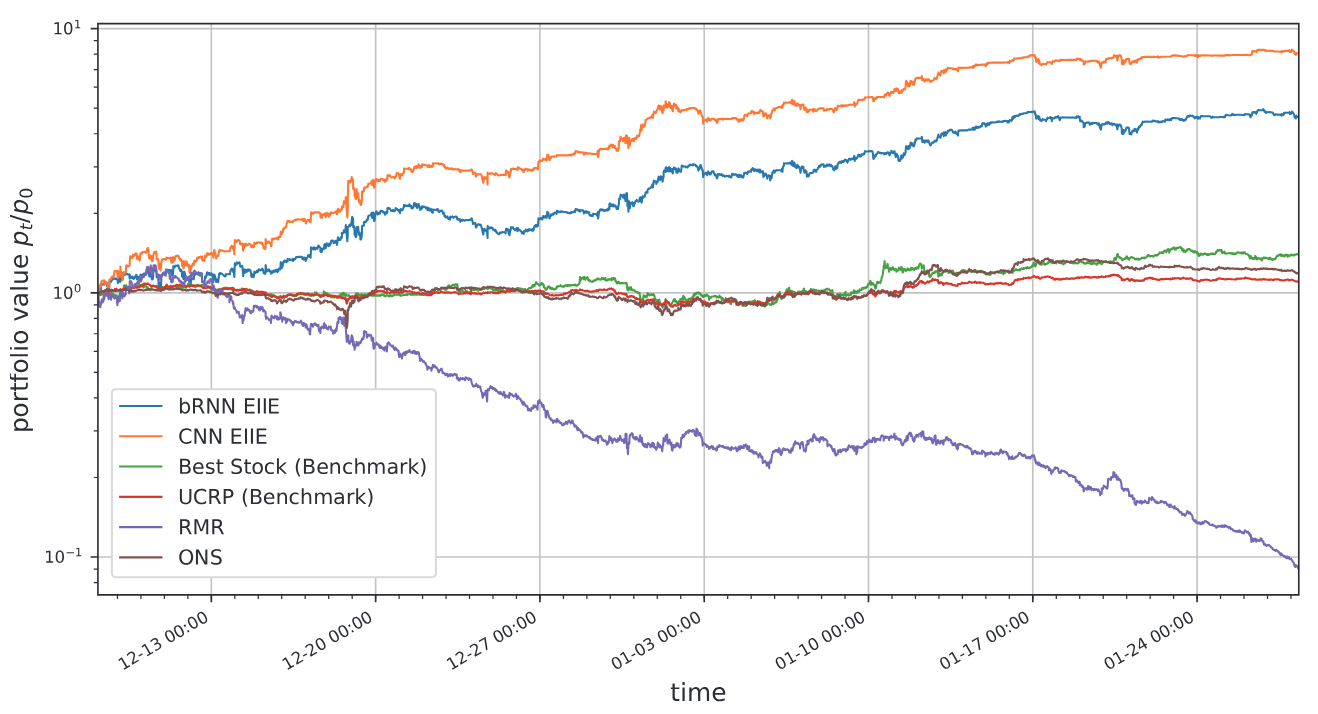
\includegraphics[width=15cm]{kep/article_eiie_result.png}
		\caption{Subset of the accumulated wealth results from the second experiment~\cite{ADRLFFPMP}.}
		\label{fig:eiie_results}
	\end{center}
	\end{figure}

	The authors highlighted the limitations of the proposed system, mentioning issues such as the system assuming no market impact or slippage, which are unrealistic. However, the proposed system still remains a highly complex, high performing proof of concept for automated trading systems.

	\subsection{Stock Market Analysis and Prediction Using LSTM: A Case Study on Technology Stocks~\cite{LiYuXuLiuMo2023}}
	This paper focuses on predicting the closing prices of certain stocks using an LSTM based neural network model. The data was sourced from Yahoo Finance using the \textit{yfinance} Python library, a free and open source module for fetching Yahoo Finance data~\cite{yfinance}. The study analyzes the closing prices of four major companies: Apple Inc. (AAPL), Google LLC (GOOG), Microsoft Corporation (MSFT) and Amazon Inc. (AMZN) from January 1, 2012, to the paper's publication in 2023.

	The first step was data preprocessing. This involved extracting the closing price data from the dataset and rescaling it to a range of 0-1. The data was then split into training and test sets with a 95\%-5\% ratio. The final preprocessing step was sequence creation, where input sequences consisted of 60 days' worth of closing prices and the corresponding target was the closing price of the 61st day.

	The neural network architecture included an input layer capable of accepting the 60 day long sequences, followed by two LSTM layers and two dense layers. The first LSTM layer had 128 neurons and returned sequences (so all hidden states over time steps) to feed into the next layer. The second LSTM layer had 64 units and returned only the last state. The final two dense layers had 25 and 1 units, respectively, with the last layer outputting the predicted closing price.

	During training, the network used the Adam optimizer and mean squared error (MSE) as the loss function. The training data was divided into batches of size 1, and the entire training process lasted for a single epoch. Model evaluation on the test set used root mean squared error (RMSE) to measure prediction accuracy~\cite{LiYuXuLiuMo2023}.

	While the model did not accurately predict closing prices, it was able to capture stock price trends with a reasonable degree of accuracy, as shown in Figure~\ref{fig:evalutaion_SMAPUL}.
	
	\begin{figure}[H]
	\begin{center}
		\includegraphics[width=\linewidth]{kep/SMAPUL.png}
		\caption{One instance from the evaluation of the proposed model~\cite{LiYuXuLiuMo2023}. The image was upscaled for better readability.}
		\label{fig:evalutaion_SMAPUL}
	\end{center}
	\end{figure}
	The predicted curve (shown in purple) mostly followed the actual test data curve (shown in blue). Being able to predict the trend of a stock price, even without knowing the exact price, is still potentially highly valuable in trading. Knowing whether a stock will generally move up or down allows traders to position themselves accordingly and profit from directional moves.

	This concept forms the basis of trend following trading strategies. A trend refers to the general direction in which an asset's price moves over time. Trend following strategies typically involve buying assets in uptrends and selling them in downtrends, aiming to capitalize on sustained price momentum rather than predicting exact prices~\cite{TFTSS}.

\chapter{Implementation of the Trading Algorithm}

\section{The Goal of the Thesis}
	Our goal is to examine how real stock market data can be used to construct trading strategies that achieve abnormal profits using neural networks. To simplify the problem, we focus more on generating profit rather than maximizing it.

	The first step is data processing. We need to transform the available raw data into a format suitable for training and testing the constructed models. For the data processing we aimed to test multiple methods to give the model the best chance to recognize and learn patterns in price fluctuations.

	To achieve our goals, we focused on supervised learning, specifically treating it as a classification problem. That is, the model outputs a trading action based on the received input. However, based on the results of previously discussed papers and projects, we also created and tested a simple setup for reinforcement learning with RNNs. For the classification approach, we opted to try both a CNN and an RNN implementation. While CNNs are primarily used for image data, we discussed how efficient CNNs are for capturing patterns in the available data, as seen in the results of the previously discussed paper in section \ref{paper_ADRLFFPMP}. For the RNN approach, we used a simple LSTM based neural network.

\section{Development Tools}
	\subsection{Development Framework}
	MATLAB\textsuperscript{\textcopyright} is a numeric computing environment that provides a wide range of tools and utilities, including a programming language, an integrated development environment (IDE) for code editing, interactive apps, and specialized libraries for solving domain-specific problems such as image processing, control system design, and data analysis. With its built-in functions and pre-made algorithms, MATLAB is widely used by engineers and researchers to design, develop, and operate complex systems across various industries. Applications include, but are not limited to autonomous vehicles, aircraft, marine vehicles, spacecraft, semiconductor design, wireless communication systems and manufacturing optimization~\cite{WhatIsMATLAB}.

	MATLAB offers another product called Simulink, which provides tools for Model-Based Systems Engineering (MBSE). Simulink enables developers to design, simulate, and deploy systems following a model-based architecture. It is primarily used to virtually simulate systems before physical testing or hardware deployment, evaluate system designs and compose control architectures~\cite{WhatIsSimulink}. Simulink is also utilized for creating machine learning systems through reinforcement learning. Using this package, intelligent agents can be trained via the standard trial-and-error interactions with dynamic environments~\cite{SimulinkAI}. 

	MATLAB is not a free product but offers various license types with different pricing, including a free license for students at partner institutions~\cite{MATLABPricing}. Due to its extensive tools and libraries, as well as the availability of the free student license, we chose MATLAB (version R2024b) as the framework for developing the program for this thesis.

	The program was developed on a PC running Debian 12 (Bookworm). The hardware specifications include an Intel Core i7-8700K CPU (4.70 GHz), an NVIDIA GeForce RTX 2070 SUPER GPU and 16 GB of RAM.

	\subsection{The Raw Data}
	The Trader Workstation (TWS) is an online platform created by Interactive Brokers (IBKR) that traders and investors use to trade stocks, bonds, futures, and more across over 150 markets worldwide via its graphical user interface~\cite{TW}. TWS also offers a non-graphical API designed for fast-paced, data-sensitive, and complex programmatic trading. This API can handle thousands of market data streams simultaneously while allowing users to execute trades~\cite{IBKRAPI}.

	Using this API, various types of data can be collected, including "Top Market Data" (Level 1) and "Market Depth" data (Level 2) for a selected instrument's limit order book. Level 1 data includes the best bid and ask prices, along with the number of shares that traders are trying to buy or sell. It essentially represents the top of the limit order book for both sides~\cite{IL1}. Level 2 data expands the information provided by Level 1 by adding the market depth, typically showing about 5-10 additional price levels. This type of data includes not only the best bid and ask prices but also some of the subsequent lines in the limit order book~\cite{IL2}.

	Generally, there are two common methods for collecting order book data: requesting full snapshots of the limit order book or receiving updates through streams of messages. The latter offers a more optimized approach, as repeatedly requesting full snapshots in a liquid market would impose a high computational load due to the large number of changes occurring every second. To mitigate this, the full snapshots are returned at discrete time intervals. However, the downside is that between snapshots, it's impossible to track the changes, significantly reducing the available information~\cite{TLOB}.

	A subset of the IBKR API, known as the TWS API, enables the collection of market data, including real-time prices, volumes, and order book information as a stream of messages. In the case of LOB data, initially, all available rows of the LOB are delivered to the client as messages, but as the market moves, only updates are sent. As previously mentioned, each message includes a single LOB update and contains the order's ID, date, type, price, and size~\cite{TWSAPIMD}. These messages were collected by László Marák, PhD, the supervisor of this thesis with the help of The Intelligent Robotics Centre at J. Selye University, using the IBKR API, starting in early 2020. The messages are organized and stored in a MySQL database.

	We tried two types of data processing methods for creating the training data. One approach involves reconstructing the limit order book with 3 level depth. This approach will be referred to as the \textit{LOB method}. The other approach uses only the theoretical value of the stock and it will be referred to as the \textit{tick price method}. 
	
	For both methods, we generate sequences where each neighbouring sequence differs by a single time step. Furthermore, we annotate the data with \textit{Buy} and \textit{Hold} labels. For annotation we check if prices surpass a defined threshold within a selected time interval from a given point. So ideally, the model's \textit{Buy} response indicates that, starting from that point, the instrument can be \textbf{sold} at a profit defined by the selected threshold value within the interval. Thus in our case, avoiding a separate \textit{Sell} label reduces redundancy and simplifies the problem.

	\subsection{Tick Price Method}
	The messages collected via the IBKR API don't have uniform time difference between them. The gaps can range from a few milliseconds to several seconds. These irregularities can make it harder to recognize patterns in price fluctuations and may cause the model to misinterpret time gaps as meaningful signals. To address this issue, we created two versions of this method: one uses interpolated stock prices (the \textit{interpolated version}) and the other uses raw stock prices with delta time appended (the \textit{raw version}). The initial steps are identical for both variants and the difference will be explained in detail later in this section.

		\subsubsection{Querying and Preparing Data}
		The data collected via the IBKR API includes a type of information called \textit{Mark Price}, defined as the current theoretical value of an instrument~\cite{TT}. We load this data from our database using SQL queries on the tables \texttt{Instrument} and \texttt{tickPrice}. The structure of these tables is shown in Figure \ref{fig:instrument_tick_price}.
		\begin{figure}[H]
		\begin{center}
			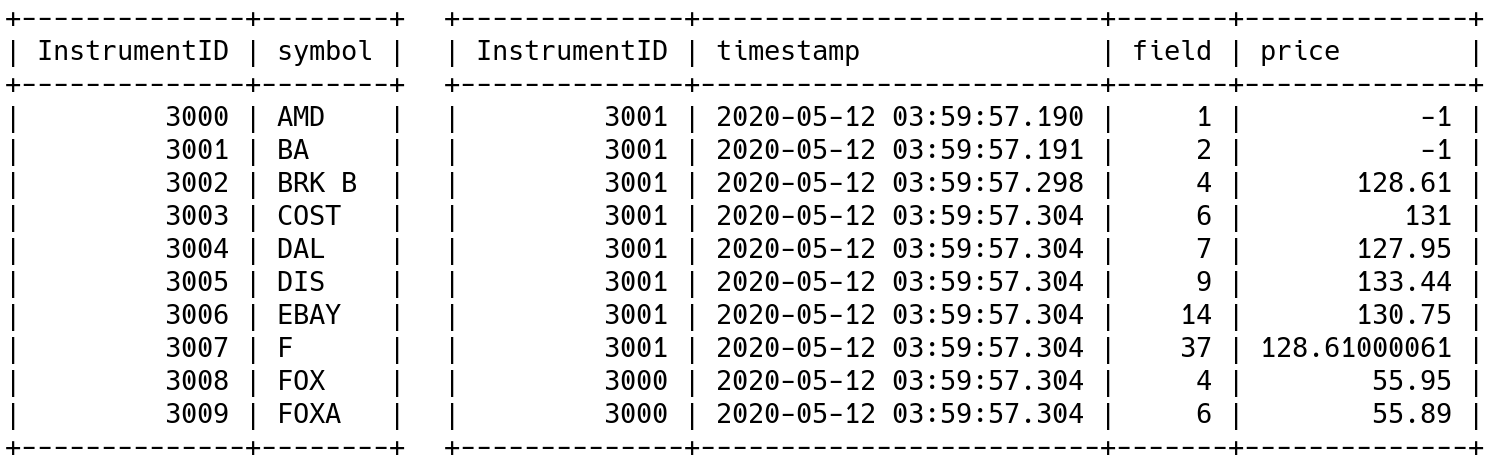
\includegraphics[width=\linewidth]{kep/table_instrument_tick_price.png}
			\caption{Structure of the \texttt{Instrument} table (left) and \texttt{tickPrice} table (right).}
			\label{fig:instrument_tick_price}
		\end{center}
		\end{figure}
		The \texttt{Instrument} table stores the numeric ID and stock symbol for each instrument and is used to indentify which message belongs to which stock. The columns of the \texttt{tickPrice} table is as follows:
		\begin{enumerate}
			\item \texttt{InstrumentID} = A numeric ID identifying the stock associated with the message.
			\item \texttt{timestamp} = The time at which the message was received.
			\item \texttt{field} = The type of message/tick. Each value represents a different type of market data, e.g. 4 defines the last price at which the instrument traded, 9 defines the closing price of the previous trading day, 14 defines the opening price, 37 defines the current theoretical value of the instrument, etc~\cite{TT}. 
			\item \texttt{price} = The value of the market data specified by the \texttt{field} column.
		\end{enumerate}
		
		As an example, using these tables, we can can determine that the closing price of BA (The Boeing Company, identified with the ID 3001 in the \texttt{Instrument} table) was \$133.44 on May 11, 2020.

		To query this data, we first specify the stock symbol, the start day timestamp, the number of days to query, and the desired market data type. In this method, we focus on the theoretical price, identified by field type 37. Starting from the first day's timestamp, we iterate through each day, querying data for regular market hours, converting timestamps to a “seconds since midnight” format for easier processing, and saving the results to separate files. This is repeated for the specified number of days.

		\subsubsection{Processing Data}
		Before starting the data processing, we check whether data from a previous run are still present. If so, we delete them to avoid potential data conflicts caused by changes in processing parameters.
		
		For the processing, 7 parameters need to be specified:
		\begin{itemize}
			\item \texttt{symbol} = The stock symbol of the selected instrument.
			\item \texttt{interpolate} = A boolean value indicating whether to process the raw data using the interpolated or raw version of the tick price method.
			\item \texttt{price\_diff\_threshold} = A threshold for identifying significant price changes (measured in percentage).
			\item \texttt{price\_diff\_margin} = A margin used to further differentiate significant price changes (measured in percentage).
			\item \texttt{future\_price\_check} = Specifies the size of the time window used to check for significant price movements (measured in seconds).
			\item \texttt{sequence\_length} = Specifies the number of time steps in each input sequence.
			\item \texttt{num\_days} = Specifies the number of days to process for training and testing.
		\end{itemize}

		We load the specified number of days' worth of data, as defined by the \texttt{num\_days} parameter. Each day's data is stored as a separate element in a cell array and processed individually.

		The first step of processing is to extract the timestamp values, which were previously converted to a "seconds since midnight" format. We define a time interval by adding 1800 seconds to the first timestamp and subtracting 1800 seconds from the last. All data outside this interval is discarded, effectively removing the first and last 30 minutes of each trading day.
		
		The opening and closing hours are typically the most volatile periods of the stock market. At the open, the market reacts to news and events that occurred since the previous day's close. Near the close, trading activity can see a surge as institutional investors and day traders close their positions. Although many day trading strategies specifically target these periods~\cite{BTDWMTS}, their high volatility may introduce noise that makes it harder for our models to learn stable patterns. For this reason, we chose to exclude them from the training data.

		If the \texttt{interpolate} parameter is set to \texttt{true}, prices are interpolated within the defined time interval using the raw data. After interpolation, the data is evenly spaced with 1 second intervals between points.

		To annotate the raw prices, we inspect each point individually. In a dataset with $n$ points, let the current point be $\text{point}_i$ with timestamp $\text{time}_i$ and price $\text{price}_i$. We define a price inspection window that starts at $\text{point}_{i+1}$ (with timestamp $\text{time}_{i+1}$ and price $\text{price}_{i+1}$) and ends at $\text{point}_j$, where $j > i$, $j \leq n$, and $\text{time}_j \leq \text{time}_i + \texttt{future\_price\_check}$. Within this window, let the highest price be $\text{price}_{\text{max}}$.

		We then compute two thresholds relative to the current price:

		\begin{align*}
		\texttt{max\_thr} &= \text{price}_i \cdot \left(1 + \frac{\texttt{price\_diff\_threshold}}{100}\right) \\
		\texttt{max\_margin\_thr} &= \text{price}_i \cdot \left(1 + \frac{\texttt{price\_diff\_threshold} - \texttt{price\_diff\_margin}}{100}\right)
		\end{align*}

		We check whether $\text{price}_{\text{max}}$ exceeds $\texttt{max\_thr}$. If it does, we label $\text{point}_i$ as \textit{Buy}. If $\text{price}_{\text{max}}$ is below $\texttt{max\_margin\_thr}$, we label $\text{point}_i$ as \textit{Hold}. Points where
		\[
		\texttt{max\_margin\_thr} < \text{price}_{\text{max}} < \texttt{max\_thr}
		\]
		are discarded. The parameter \texttt{price\_diff\_margin} thus creates a buffer zone between \textit{Buy} and \textit{Hold} signals, which we test to see if it helps the model better differentiate these labels.
		
		Figure~\ref{fig:margin_thr} illustrates the \texttt{price\_diff\_margin} and \texttt{price\_diff\_threshold} on simulated prices.
		\begin{figure}[H]
		\begin{center}
			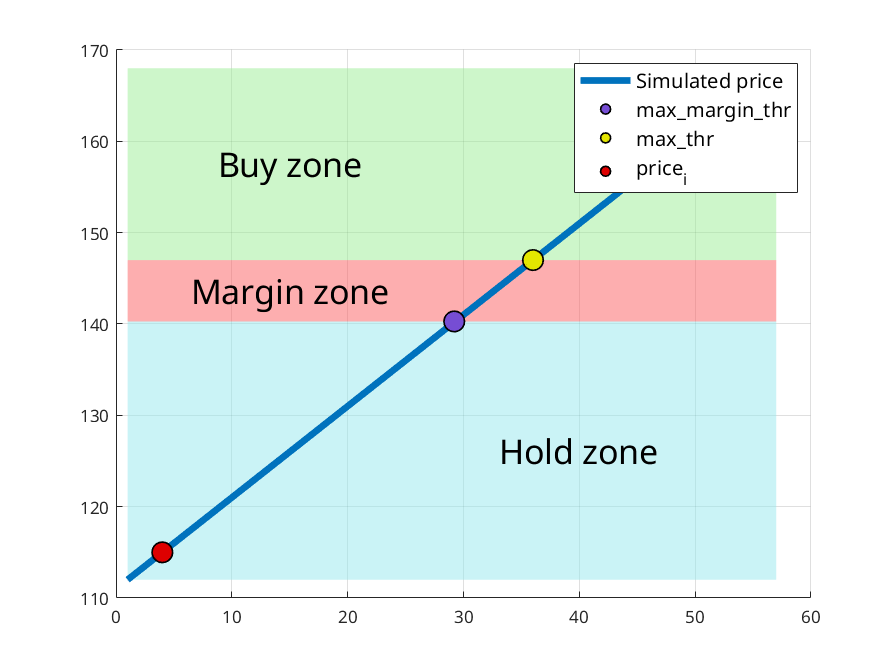
\includegraphics[width=12cm]{kep/margin_thr.png}
			\caption{Illustrating \texttt{price\_diff\_margin} and \texttt{price\_diff\_threshold} on simulated prices.}
			\label{fig:margin_thr}
		\end{center}
		\end{figure}

		Annotating interpolated prices is simpler because each step differs by exactly one second. Starting from the current point $\text{point}_i$, we define the inspection window as the next \texttt{future\_price\_check} time steps. The annotation logic remains the same as in the raw version.

		After annotating the last day, the sequence creation step begins. To create sequences, we iteratively take \texttt{sequence\_length} number of prices from the annotated data and normalize them using z-score normalization. Each sequence is stored separately as an array element.

		When creating sequences from raw prices, we also calculate the delta time. For $\text{point}_i$, the delta time is defined as $\Delta\text{time}_i = \text{time}_i - \text{time}_{i-1}$. The delta time for the first step of each sequence is set to 0. This means that, alongside the raw prices, we save additional data indicating the time elapsed since the previous point. 

		When creating sequences from interpolated prices, the result is an $N \times \texttt{sequence\_length} \times 1$ array, where $N$ is the number of sequences generated from that day's data, and each time step contains a normalized price. When creating sequences from raw prices, the result is an $N \times \texttt{sequence\_length} \times 2$ array, where each time step contains both a normalized price and the corresponding delta time. This structure is illustrated in Figure~\ref{fig:resulting_sequences}.
		\begin{figure}[H]
		\begin{center}
			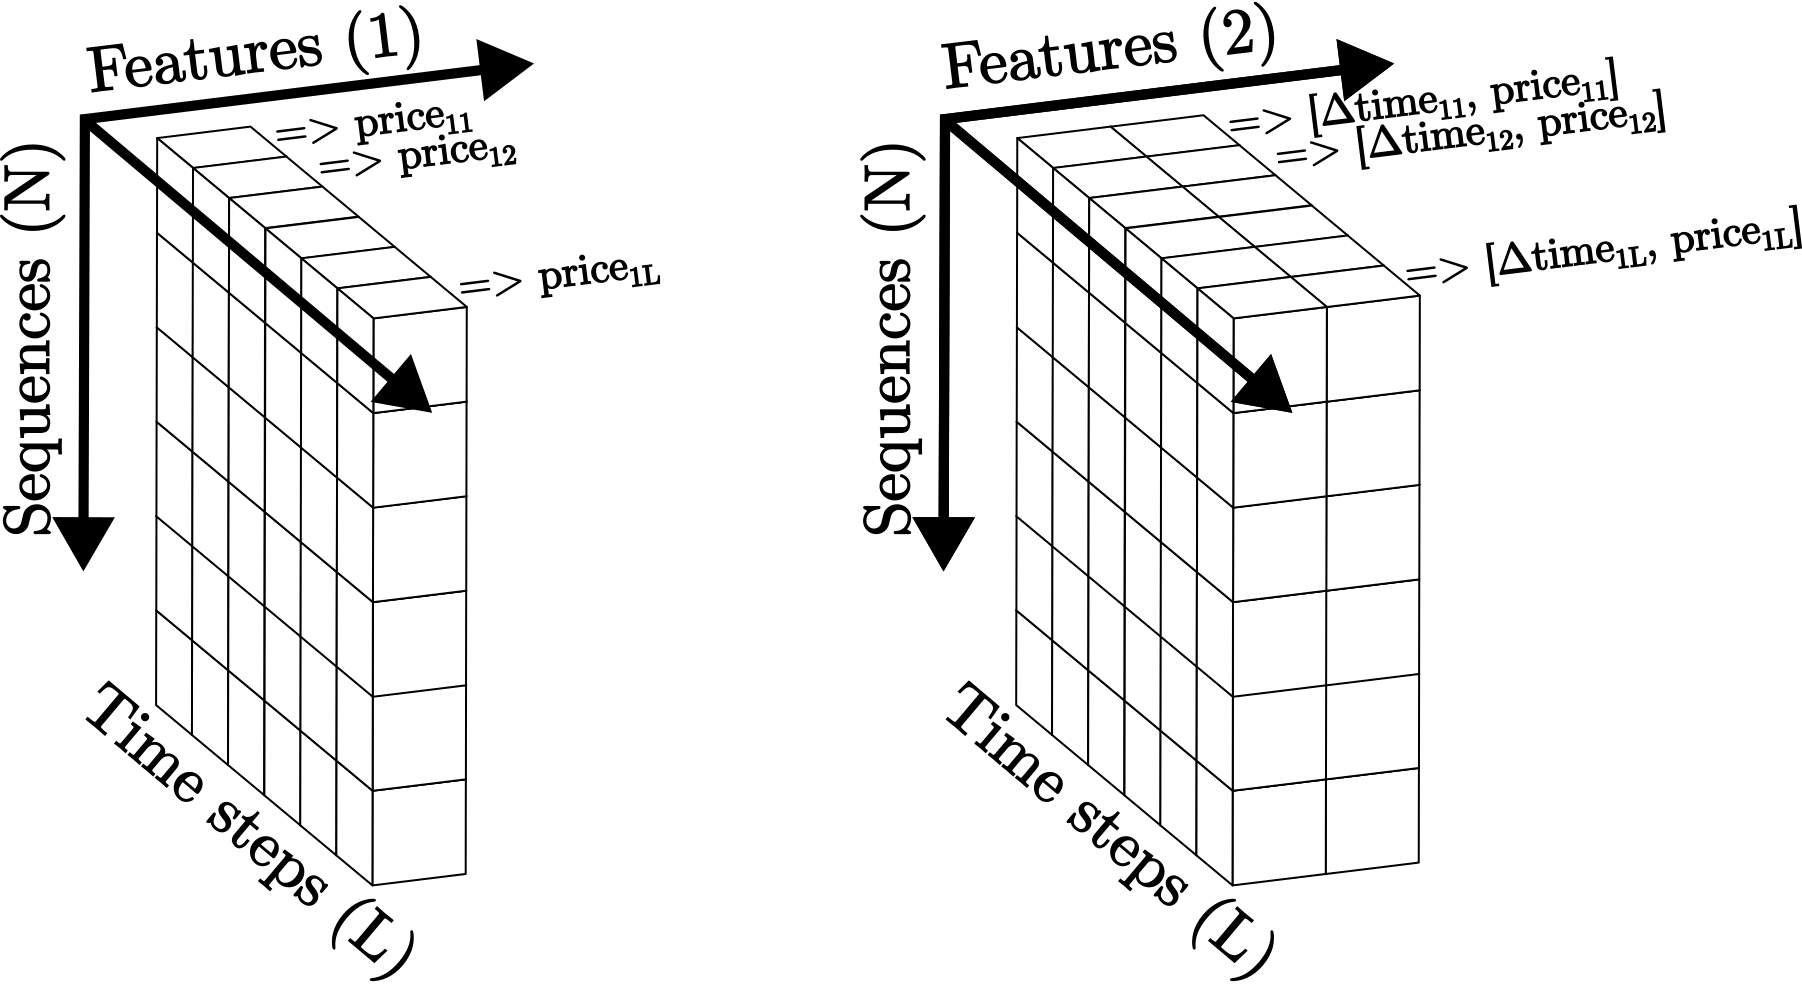
\includegraphics[width=\linewidth]{kep/resulting_seq.png}
			\caption{Structure of the resulting sequences using the interpolated (left) and raw (right) versions of the tick price method.}
			\label{fig:resulting_sequences}
		\end{center}
		\end{figure}

		The label for each sequence is assigned based on the label of its last time step. We save all sequences belonging to separate days in separate files.

		Figure~\ref{fig:ann_seq_process} illustrates the annotation and sequence creation process. Green circles mark the moments labeled as \textit{Buy}. The black cross indicates the first \textit{Buy} moment of the presented day, and its corresponding sequence is also shown. The light red area represents the price inspection window defined by \texttt{future\_price\_check} for this moment, with red asterisks highlighting the prices that exceed the \texttt{price\_diff\_threshold} within the window.
		\begin{figure}[H]
		\begin{center}
			\includegraphics[width=\linewidth]{kep/annotattion_illst.png}
			\caption{Illustration of the annotation and sequence creation process on a subset of an arbitrarily selected day. The \texttt{future\_price\_check} is set to 3600 seconds, and the \texttt{price\_diff\_threshold} is set to 1\%.}
			\label{fig:ann_seq_process}
		\end{center}
		\end{figure}

		\subsubsection{Balancing the Dataset}
		Each day can produce tens of thousands of sequences, reaching sizes of 15+ GB, making it unfeasible to load all generated sequences into the production computer's memory. Furthermore, the vast majority of sequences are labeled as \textit{Hold}. For example, in one of our tests, the class distribution between \textit{Hold} and \textit{Buy} was 95\%-5\%. Using this data directly as a training set would result in a highly imbalanced data set, which could bias the model toward the majority class and lead to poor classification of the minority class, in this case, the \textit{Buy} class~\cite{DID}.

		We attempted to address the memory issue by using MATLAB's integrated datastore repository. However, by default, datastores do not read data in structured batches as needed, and this approach still wouldn't solve the class imbalance.

		To resolve both problems, we implemented a custom balancing function. First, we count the total number of \textit{Buy} and \textit{Hold} labels across all generated files. Based on this, we calculate a quota, named \texttt{hold\_per\_file}, that determines how many \textit{Hold} samples to include per file in order to balance the overall dataset. Then, we iterate through each file (representing a day), shuffle its sequences, and separate them into \textit{Buy} and \textit{Hold} subsets. We keep all \textit{Buy} samples and keep only the first \texttt{hold\_per\_file} number of \textit{Hold} samples, then merge the two subsets. Finally, we shuffle the merged set to remove any class ordering.

		We repeat this process for all available days except the last two. The last day is reserved as the test set, while the second-to-last is used for validation. Both are kept imbalanced to evaluate how well the model generalizes to real world data. The effects of balancing on the tranining set are shown in Figure~\ref{fig:un_balanced_dataset}.

		\begin{figure}[H]
		\begin{center}
			\includegraphics[width=\linewidth]{kep/dataset.png}
			\caption{A training set before (left) and after (right) balancing.}
			\label{fig:un_balanced_dataset}
		\end{center}
		\end{figure}

	\subsection{LOB Method}
    This method will be used to create the environment for the reinforcement learning implementation and to create a learning set similar to the one generated using the tick price method for classification, but with more features to provide the model with additional information to help it learn patterns. The process of creating the classification set is identical to that of the reinforcement learning set, with additional steps at the end.
		\subsubsection{Querying and Preparing Data} 
			For the LOB reconstruction we use two tables from our database: \texttt{reqMktDepth} and \texttt{updateMktDepthL2}. The latter contains the limit order book message streams, while the \texttt{reqMktDepth} table stores the tickerID-stock symbol pairs needed to identify which message belongs to which stock.

			\begin{figure}[H]
			\begin{center}
				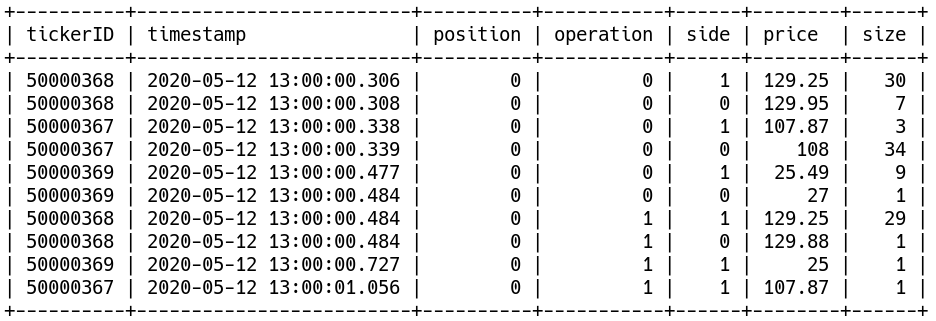
\includegraphics[width=\linewidth]{kep/updateMktDepthL2.png}
				\caption{Structure of the \texttt{updateMktDepthL2} table, showing only the first 10 entries.}
				\label{fig:updateMktDepthL2}
			\end{center}
			\end{figure}

			In Figure~\ref{fig:updateMktDepthL2}, we can observe the structure of the messages. The meaning of each column is as follows:
			\begin{enumerate}
				\item \texttt{tickerID} = A numeric ID identifying the stock associated with the message. 
				\item \texttt{timestamp} = The time at which the message was received. 
				\item \texttt{position} = Indicates the position where the update should be performed in the order book (starting at index 0). 
				\item \texttt{operation} = Specifies the operation to be performed. Three types of operations are possible: insert, update, and delete, each coded numerically starting from 0 to 2 respectively. 
				\item \texttt{side} = Specifies the side of the limit order book where the operation should be performed. The sides are coded numerically: 0 is the ask book, 1 is the bid book. 
				\item \texttt{price} = The value of the given order. 
				\item \texttt{size} = The quantity of the stock being traded. 
			\end{enumerate}

			As already mentioned, the \texttt{tickerID} identifies the limit order book, and each \texttt{tickerID} is paired with a stock symbol. However, this \texttt{tickerID} is not constant for the symbols, it changes with each request. To properly identify the limit order books, the previously mentioned \texttt{reqMktDepth} table is required.
			\begin{figure}[H]
			\begin{center}
				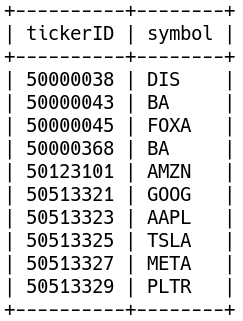
\includegraphics[scale=0.75]{kep/reqMktDepth.png}
				\caption{Structure of the \texttt{reqMktDepth} table, showing only the first 10 rows.}
				\label{fig:reqMktDepth structure}
			\end{center}
			\end{figure}

			Figure~\ref{fig:reqMktDepth structure} shows the simple structure of the \texttt{reqMktDepth} table, which consists of two columns: the first column stores the \texttt{tickerID}, and the second column displays the symbol pair associated with the \texttt{tickerID}s. Using this table, we can determine that the first two messages, as well as the third and fourth messages from the back of the table shown in Figure~\ref{fig:updateMktDepthL2}, belong to the symbol \textit{BA}, which as already mentioned, represents The Boeing Company on the stock market.

			Before querying the required data, we first specify the start and end time of the desired data interval and select the stock symbol for which we want to reconstruct the LOB.

			Once the necessary variables are initialized, we retrieve all ticker IDs matching the specified time interval and stock symbol. We then iterate through these ticker IDs. Each ticker ID represents a separate, disjunct requests of the LOB, and their messages shouldn't be mixed. To avoid this, we only process messages from one ticker ID at a time. After reaching the last message of a given ticker ID, the reconstruction restarts from an empty LOB, ensuring that messages from different ticker IDs are not mixed.

			After querying the messages for a given ticker ID, timestamps are converted to MATLAB's datetime format, and the position values in the messages are incremented by 1. This is necessary because the positions originally start from index 0, but MATLAB tables don't support indexing from zero.

		\subsubsection{Reconstructing the LOB}  
			Once the data is queried and prepared, the reconstruction begins. We create two empty tables: one for the ask side and one for the bid side of the LOB. Then, we iterate through the messages and execute the specified operation of each message on the appropriate side of the LOB. The operations are handled as follows:
			\begin{itemize}
				\item \textbf{Insert operation} = MATLAB does not have a built-in function to insert a row into a table, so this operation is implemented manually. If a message needs to be inserted at index $n$, the table is split into two parts: one from the start to index $n-1$ and another from index $n$ to the end. The new message is then inserted between these two segments, reconcatenating the table.  
				\item \textbf{Update operation} = This is handled by simply overwriting the existing row.  
				\item \textbf{Delete operation} = This is performed using MATLAB's built-in table row deletion functionality.  
			\end{itemize}

		\subsubsection{Generating LOB Snapshots}
			To train our neural network we need to create a training set with a sufficient amount of data. The training set is generated by capturing snapshots of the LOB as it is being built.

			An important aspect of snapshot generation is determining when the snapshots should be taken, specifically the time interval between subsequent snapshots. Our implementation processes all operations occurring at the same time with integer-second precision before generating a snapshot. This method produces a large number of snapshots while minimazing redundancy and data loss.

			After creating a snapshot, we check the prices of each order in the LOB and aggregate the sizes of orders that share the same price. This process is illustrated in Figure~\ref{fig:before_after_agg}.

			\begin{figure}[H]
			\begin{center}
				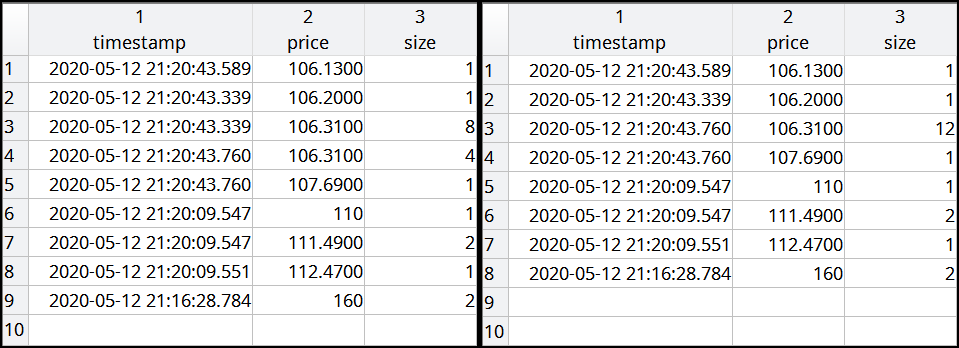
\includegraphics[width=\linewidth]{kep/lob_before_after_agg.png}
				\caption{Ask side of a LOB snapshot before (left) and after (right) aggregation.}
				\label{fig:before_after_agg}
			\end{center}
			\end{figure}

		\subsubsection{Formatting the Snapshots}\label{section_FS}
			To effectively use the LOB snapshots programmatically, we format each generated snapshot similarly to the format used by the previously described limit order book reconstruction tool, LOBSTER. Each snapshot becomes a row in a table, with the first column storing the latest timestamp of the snapshot. This timestamp, like in the tick price method, is converted to a “seconds since midnight” format and snapshots outside regular trading hours are filtered out. The remaining columns alternate between ask and bid information: ask price 1, ask size 1, bid price 1, bid size 1, then ask price 2, and so on, up to a specified depth. For our tests, we specified the depth as level 3, meaning we use the first three levels of the limit order book. As we process each snapshot, we vertically concatenate it with the previously processed ones. The structure of the formatted snapshots is shown in Figure \ref{fig:formatted_lob}.

			\begin{figure}[H]
			\begin{center}
				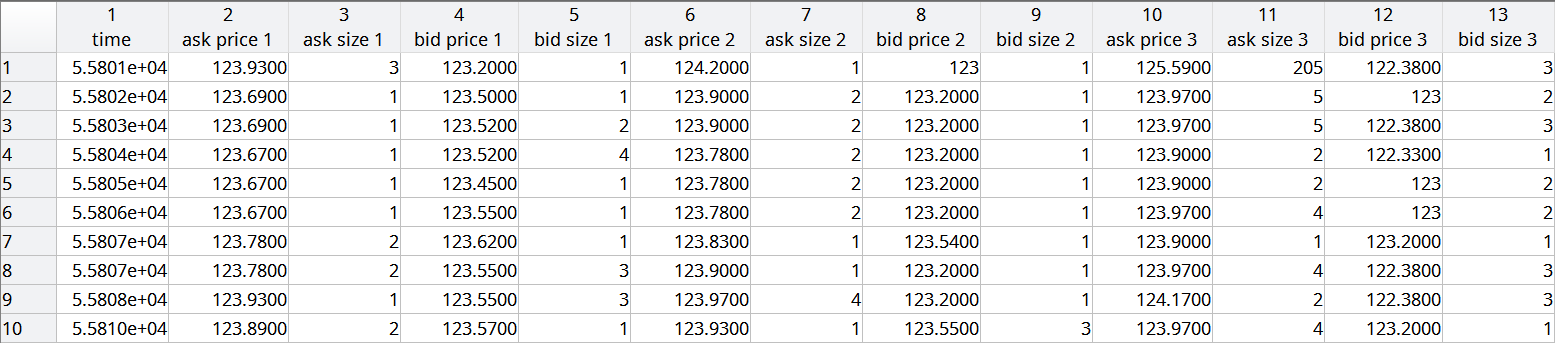
\includegraphics[width=\linewidth]{kep/formatted_lob.png}
				\caption{The first ten LOB snapshots with depth 3 from an arbitrarily selected day.}
				\label{fig:formatted_lob}
			\end{center}
			\end{figure}

			The resulting table is saved separately for each day and is used for the reinforcement learning implementation. For the classification implementation, additional processing is required.

		\subsubsection{Processing the LOB Snapshots for Classification}
		The earlier formatted LOB snapshots can be easily reshaped to fit the format required by the classification approach. This process is very similar to how we handle the raw version of the tick price method and it requires the same seven parameters.

		First, we check whether data from a previous run is still present and delete it if necessary to avoid data conflicts. Then we load the specified number of days into a cell array, with each day stored as a separate element. We also remove the first and last 30 minutes of each trading day.

		To annotate this data, we need to approximate the current price of the stock. We do this by calculating the mid price as the average of the best ask and bid prices:
		\[
		\text{MidPrice} = \frac{\text{AskPrice}_{1}\ +\ \text{BidPrice}_{1}}{2}
		\]

		The calculated mid price is used only during annotation and is not saved. After calculating the mid price, every other annotation step is identical to the one used in the raw version of the tick price method.

		The sequence creation is also similar to the raw version of the tick price method. To create the sequences from the annotated LOB snapshots, we iteratively take \texttt{sequence\_length} number of points and calculate delta time. This time, we do not have a single price value to pair with the delta time, instead, we use six prices and six order sizes from the top three levels of the LOB. The six price vectors are normalized across the time steps of the sequence using z-score normalization. Just like before, each sequence is stored separately as an array element and the label for each sequence is the label of its last time step.

		The result for each day is an array with $N \times \texttt{sequence\_length} \times 13$ dimensions, where $N$ is the number of sequences generated from that day's data. This time, each time step contains six normalized prices, six order sizes, and the delta time. Once the current day's data is processed, it is saved to a separate file before moving on to the next day.

		The vast majority of the sequences will likely have \textit{Hold} labels, so this set also requires balancing. For this, we use the excat same method as we use for the tick price method.

	\subsection{Creating the Environment and Agent for Reinforcement Learning}
	We built the reinforcement learning environment following a standard loop from a freely available MATLAB example~\cite{DRLOTE} to create a proof of concept or benchmark we can work upon later. At each time step the agent receives an observation, selects an action, and the environment transitions to a new state.

	At the start, the environment loads the preprocessed LOB data, formatted as described in Section~\ref{section_FS}, for the specified days and stock symbol. For each test, only one stock symbol is used. An episode begins with a fixed budget and zero owned stocks. We define a trading horizon of 60 seconds, meaning the agent can hold a stock for a maximum of 60 seconds before being forced to sell it, preventing the agent from holding stocks for too long. Each step in the episode corresponds to a row in the loaded LOB data. At every time step, the agent observes features representing the current market conditions and its own financial state. These features include:
	\begin{itemize}
		\item Short-term price trends = The difference between consecutive mid prices, where $t$ is the current time step: 
			\[ \text{PriceTrend}\ =\ \text{MidPrice}_{t} -\ \text{MidPrice}_{t-1} \]
		\item Simple Moving Average (SMA) = The average of recent mid prices over the past $N$ time steps:
			\[ \text{SMA}\ =\ \frac{\sum_{i=t-N}^{t}{\text{MidPrice}_{i}}}{N} \]
		\item Bid-Ask order size balance = Reflects market pressure. A negative value indicates more supply and sell pressure, while a positive value indicates more demand and buy pressure. For depth $D\ =\ 3$:
			\begin{align*}
			\text{BidSizes}\ &=\ \sum_{i=1}^{D}{\text{BidSize}_i}\\
			\text{AskSizes}\ &=\ \sum_{i=1}^{D}{\text{AskSize}_i}\\
			\text{SizeBalance}\ &=\ \frac{\text{BidSizes}\ -\ \text{AskSizes}}{\text{BidSizes}\ +\ \text{AskSizes}}
			\end{align*}
		\item Bid-Ask spread = A basic liquidity indicator. A narrow spread imply high liquidity, while a wider spread imply low liquidity:
			\[ \text{Spread} = \text{AskPrice}_{1} - \text{BidPrice}_{1} \]
		\item Volatility = The standard deviation of mid price changes. We approximate this over the last $N$ steps:
			\[ \text{Volatility} = \mathrm{std}\big( (\text{MidPrice}_{t-N+1} - \text{MidPrice}_{t-N}), \ldots, (\text{MidPrice}_{t} - \text{MidPrice}_{t-1}) \big) \]
		\item Cash in hand = Available funds for buying stocks.
		\item Stocks owned = The number of currently held stocks.
		\item Portfolio value = Total value of the agent's current portfolio:
			\begin{align*}
			\text{StockValue}\ &=\ \text{MidPrice}_{t}\ \cdot\ \text{StocksOwned}_{t} \\
			\text{PortfolioValue}\ &=\ \text{Cash}_{t}\ +\ \text{StockValue}_{t}
			\end{align*}
		\item Remaining time = Indicated how much time is left within the 60 second trading horizon.
	\end{itemize}

	The agent can choose from three actions at each time step: \textit{Buy}, \textit{Sell} or \textit{Hold}. The \textit{Buy} action uses all available cash to purchase as many stocks as possible at the best ask price. The \textit{Sell} action sells all available stocks at the best bid price. The \textit{Hold} action passes the current state without making a \textit{Buy} or \textit{Sell}.

	We aimed to design a reward function to help the agent learn profitable strategies. If the agent tries an invalid action, like selling without owning stocks or buying without enough cash, it gets a fixed and relatively big penalty:
	\[ R\ =\ -100 \]
	For valid actions, the reward depends on profitability. When selling, the reward is:
	\[ R\ =\ \lambda\ \cdot\ (\text{StockValue}_{t} - \text{StockValue}_{t+1}) \]
	The $\lambda$ component is a weight used to scale the reward. The buy action uses a similar equation, but reversed:
	\[ R\ =\ \lambda\ \cdot\ (\text{StockValue}_{t+1} - \text{StockValue}_{t}) \]
	This rewards buying before the stock price goes up and penalizes buying before it goes down. For the hold action, we aimed to design a reward function to discourage holding for too long and to avoid penalties only when prices are stable:
	\[ R\ =\ -\mid \text{MidPrice}_{t+1} - \text{MidPrice}_{t} \mid -\ \lambda\ \cdot\ \text{TimeHeld} \]
	In the equation above, TimeHeld is the time elapsed since the agent started the hold action and $\lambda$ is a weight used to scale the time penalty.

	An episode ends when the agent reaches the last time step or runs out of funds and holds no stocks.

	The agent was designed in MATLAB's Reinforcement Learning Designer using Deep Q-Learning (DQN) and a recurrent neural network with 256 hidden units. The agent's structure is shown in Figure~\ref{fig:agent_structure}.
	
	\begin{figure}[H]
	\begin{center}
		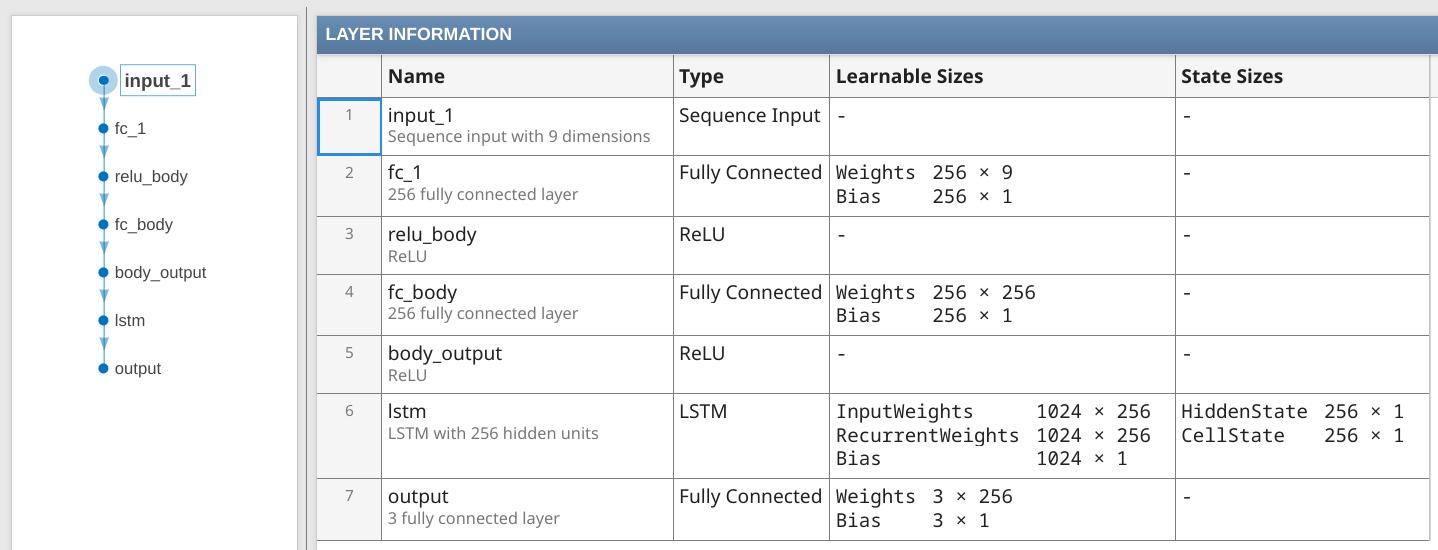
\includegraphics[width=\linewidth]{kep/agent_structure.png}
		\caption{The structure of the agent created with the Reinforcement Learning Designer.}
		\label{fig:agent_structure}
	\end{center}
	\end{figure}

	\subsection{Creating the Neural Networks for Supervised Learning}
	For supervised learning, we tested two types of models: a CNN, specifically the LeNet topology and an RNN, using an LSTM based recurrent network.

	\begin{figure}[H]
	\begin{center}
		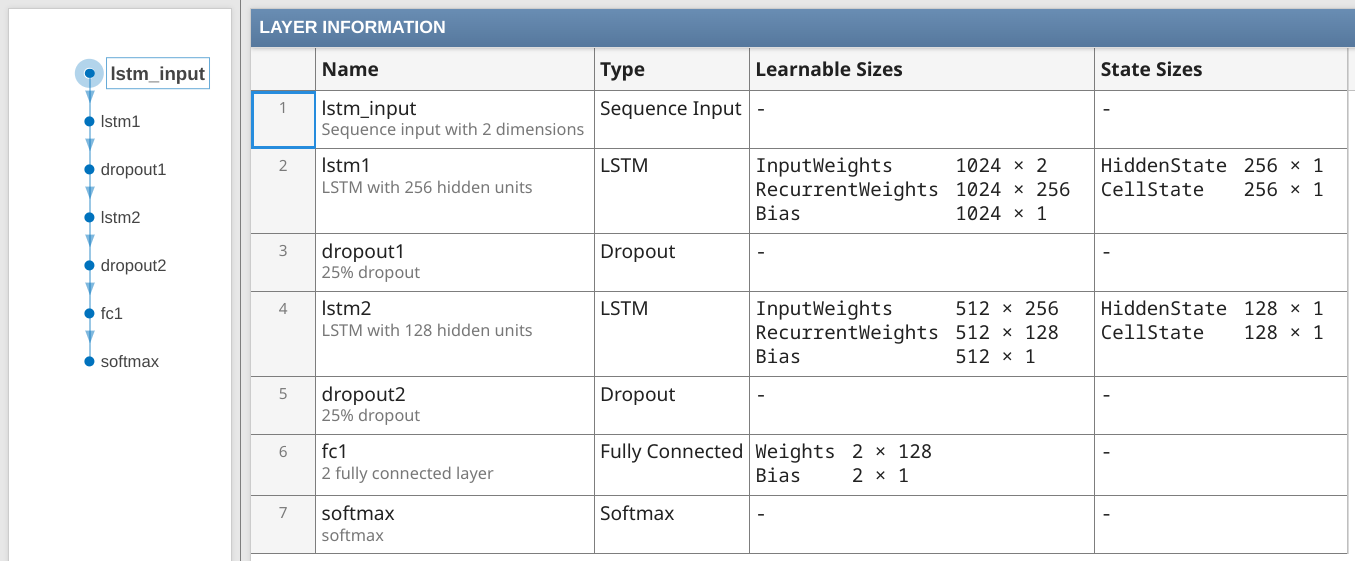
\includegraphics[width=\linewidth]{kep/lstm_structure.png}
		\caption{The structure of the LSTM based RNN. The sequence input dimension is 2 for the raw version, and 1 for the interpolated version of the tick price method.}
		\label{fig:lstm_structure}
	\end{center}
	\end{figure}

	The structure of our LSTM based network can be seen in Figure \ref{fig:lstm_structure}. Generally, a deeper LSTM model with multiple layers can learn more abstract features and patterns, though adding too many layers may lead to overfitting~\cite{DDIELL}. Our LSTM based network uses two layers: the first with 256 hidden units and the second with 128. The model performs sequence-to-label classification, where it processes a sequence and returns a single label. For this to work in a multilayer setup, the first LSTM layer has to return a sequence, while the second returns only the final output~\cite{LSTMNN}. This is done by setting the \texttt{OutputMode} to \texttt{sequence} for the first LSTM layer, and \texttt{last} for the second.

	The \texttt{dropoutLayer} after each LSTM layer reduces the chance of overfitting by generating a dropout mask. Using this mask, some input elements are set to zero, while the remaining ones are scaled by dividing by $(1 - DropoutRate)$. At prediction time, the layer passes the input unchanged~\cite{DL}. Both dropout rates in our network are set to 25\%.

	\begin{figure}[H]
	\begin{center}
		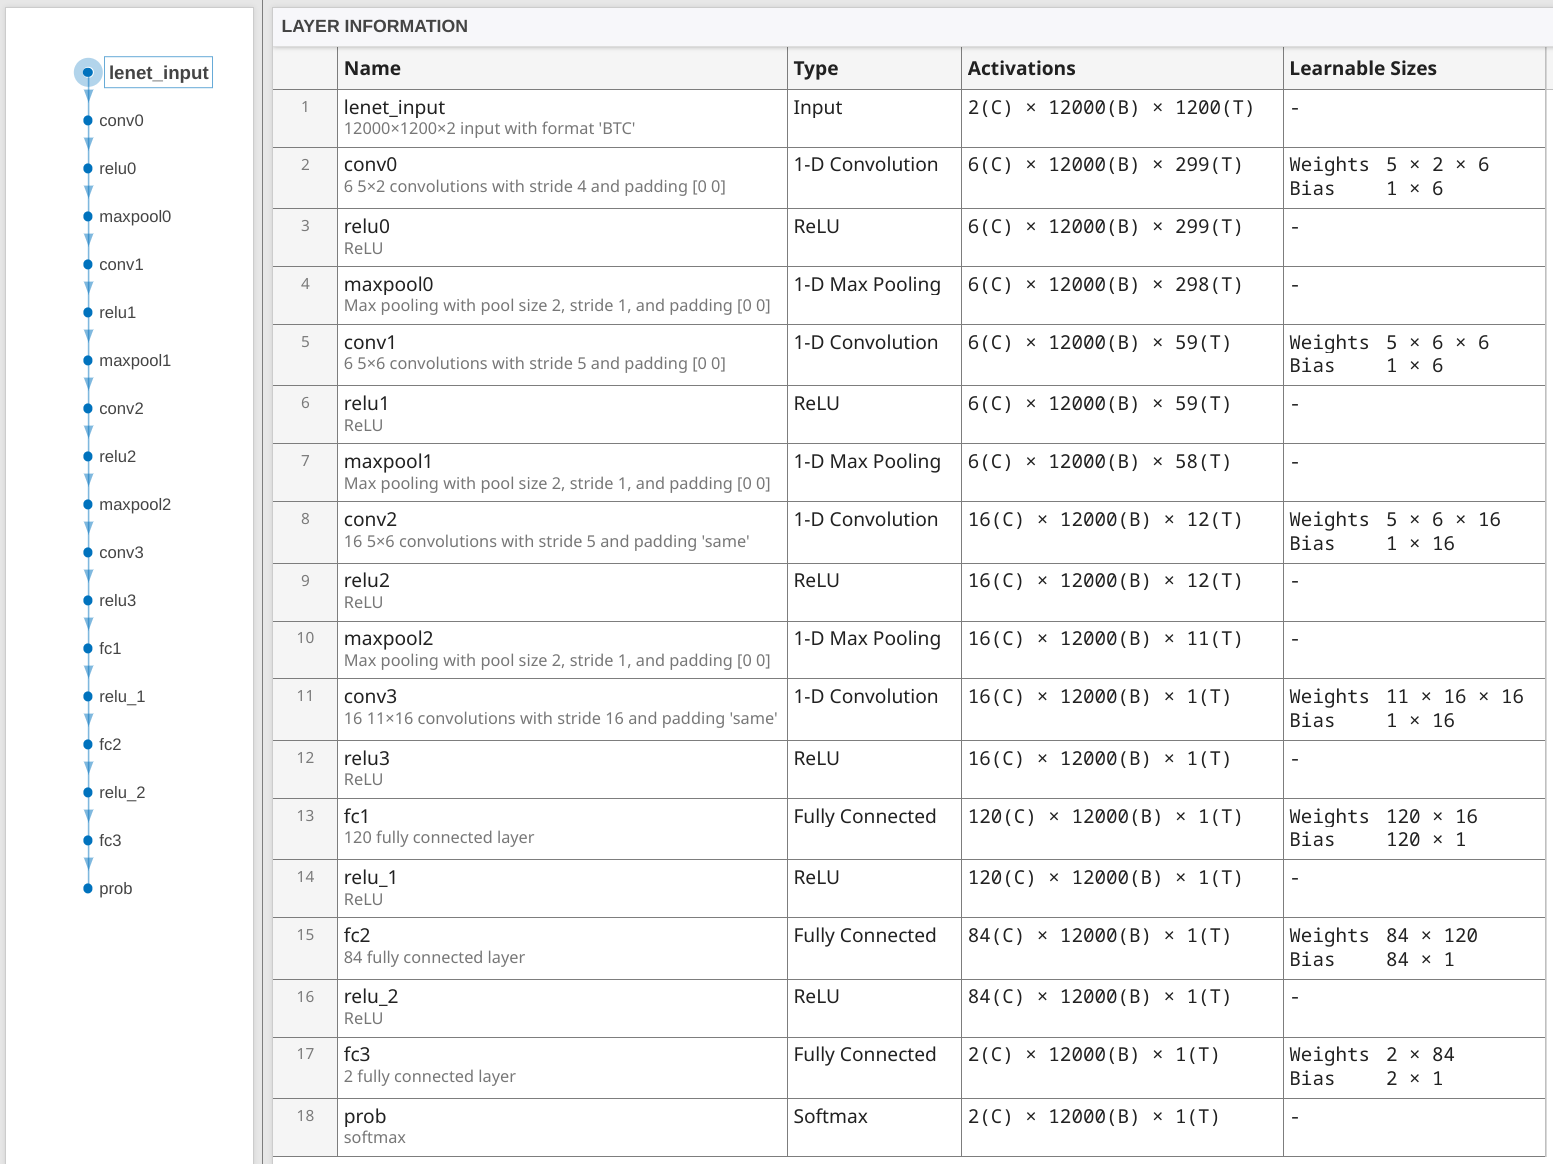
\includegraphics[width=\linewidth]{kep/lenet_structure.png}
		\caption{The structure of the LeNet based CNN with an arbitrarily chosen input dimension.}
		\label{fig:lenet_structure}
	\end{center}
	\end{figure}

	In Figure~\ref{fig:lenet_structure} the structure of our LeNet implementation is shown. The initial 1D convolution-ReLU-max pooling layer group (with index 0) is only included when processing very long sequences, otherwise it's ommited. The core of the network consists of two sets of 1D convolution-ReLU-max pooling layers, labeled with indices 1 and 2. The \texttt{conv1} layer has 6 filters with a 1x5 kernel and a stride of 5. The next convolution layer, \texttt{conv2}, uses 16 filters with the same kernel size and stride. Its \texttt{Padding} parameter is set to \texttt{same}, ensuring that the output size is $\left\lceil \frac{\text{InputSize}}{\text{Stride}} \right\rceil$, which prevents excessive shrinking of the input during convolution~\cite{1DCL}. The final convolution layer, \texttt{conv3}, also uses padding, with 16 filters, a 1x11 kernel and a stride of 16. It is followed by a ReLU and then three fully connected layers. Each max pooling layer uses a pool size of 2 to downsample the sequence.

	The \texttt{sequenceInputLayer} used in the LSTM model is incompatible with convolution layers, so we used a custom \texttt{inputLayer} instead. To ensure that MATLAB correctly interprets the input data, we set the input format (height x width x depth) using the \texttt{BTC} format. Here, the first dimension (height), which holds the individual sequences, represents the \textbf{b}atch size, the second (width) stores the \textbf{t}ime steps, and the third (depth) holds the features or \textbf{c}hannels.

	Both networks end with a fully connected layer with as many neurons as classes.

\section{Testing and Evaluating the Implementations}
After creating the base framework for the reinforcement learning and supervised learning based systems, we ran multiple tests to find the optimal hyperparameters of each implementation in a trial and error way. This chapter presents the tests and evaluates their outcomes.
	\subsection{The Reinforcement Learning Implementation}
	The adjustable environment parameters include the initial funds, reward scaling factor $\lambda$ and the window size $N$ used to compute the SMA and volatility. The training parameters to experiment with include the learning rate, batch size, exploration epsilon, decay rates for learning and exploration, and the number of epochs.

	Even after a limited number of tests, it became clear that the agent could not learn any meaningful patterns from the data. Regardless of the parameters used, it seemingly chose randomly from the three trading actions. Figure~\ref{fig:rl_episode_rewards} shows the agent's accumulated rewards across episodes in one of the tests runs. The worst case cumulative reward is $-5 \cdot 10^4$.

	\begin{figure}[H]
	\begin{center}
		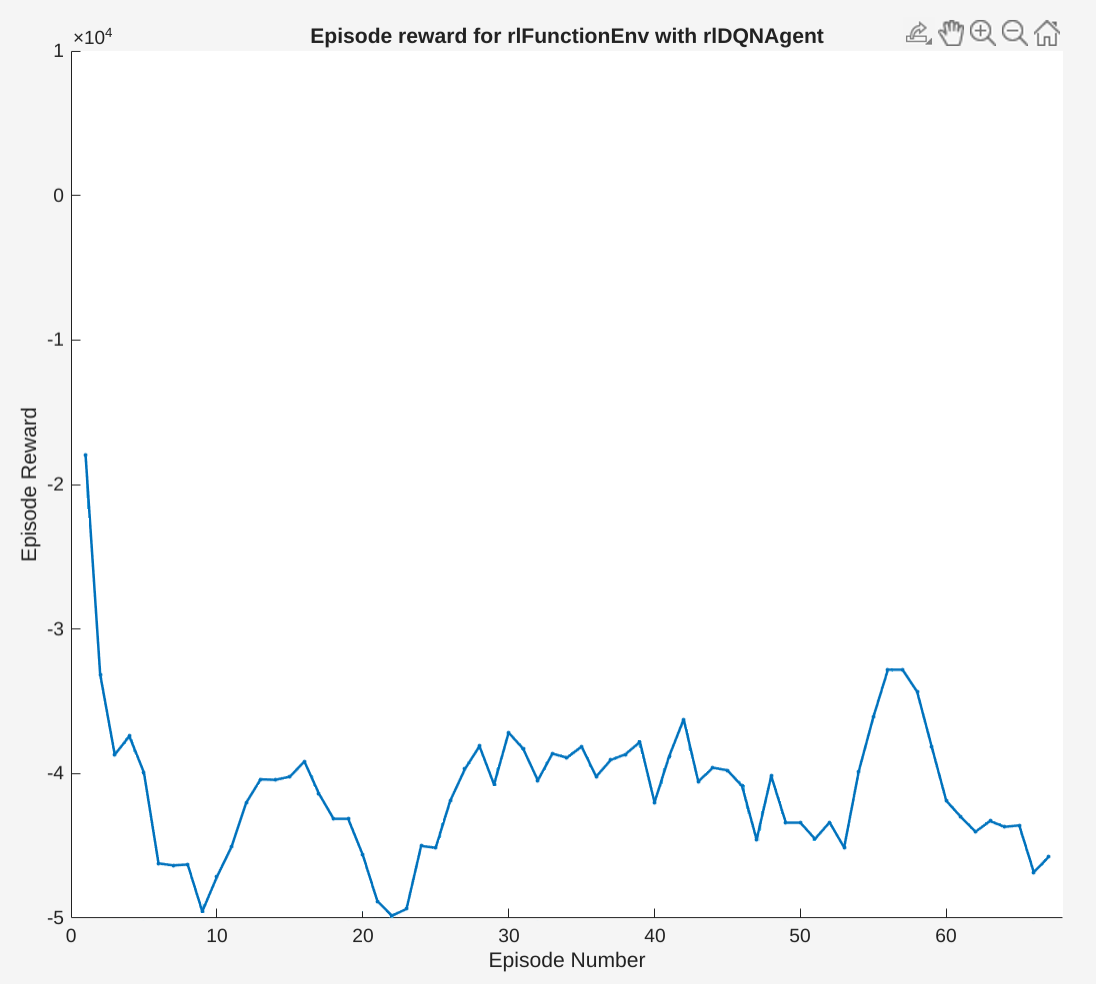
\includegraphics[width=0.9\linewidth]{kep/RL1_episode_rewards.png}
		\caption{The accumulated rewards in one test.}
		\label{fig:rl_episode_rewards}
	\end{center}
	\end{figure}

	Despite various parameter adjustments, the agent consistently failed to learn a usable trading strategy. It did learn to avoid illegal actions, but nothing beyond that. Since changing parameters had no effect, we concluded the issue likely stemmed in the structure of both the learning process and the environment. 

	The penalty for illegal actions was fixed and relatively large, which might have overshadowed the smaller profit-based rewards. This could result in the agent learning only what not to do, without enough motivation to explore good strategies. The reward for the hold action also penalized both market volatility and the time spent holding. In some periods, this may have discouraged the agent from holding even when it would have been beneficial.
	
	The environment itself may also have contributed to the failure. The 60 second trading horizon forced the agent to make decisions within a short time window, preventing it from learning longer-term strategies, adapting to slower market changes, and possibly introducing noise due to the small time frame. It also introduced a constraint that doesn't necessarily reflect real trading conditions, where timing flexibility is often crucial.

	The observation space, while covering some key features such as short-term trends, SMA, might not have provided enough information for the agent to understand market context. With limited inputs and no access to more complex patterns or long term trends, the agent may have lacked the informations needed to learn profitable behaviours. Additionally, the way financial state features, such as cash and portfolio value, were represented might have made it difficult for the agent to connect its actions with long-term outcomes during training.
	
	As our main focus is the supervised learning approach, we decided not to redesign the reinforcement learning environment and proceeded with the insights gained. Based on our experiences with this setup, the supervised learning implementation uses a longer prediction horizon than the 60 seconds used in the reinforcement learning tests. This should reduce noise and help the model capture more meaningful patterns.

	\subsection{The Supervised Learning Implementations}
	The primary goal of these tests is to compare the performance of the two network architectures (LSTM and LeNet) and two data processing methods (LOB method and tick price method), as well as to find the optimal parameters. To ensure fair comparisons, we tested the networks using the same parameters and datasets whenever possible.

	The tunable data processing parameters include the price interpolation flag, price threshold for identifying significant changes, price margin, window size for checking future prices, and sequence length. The only training parameter varied between tests was the mini-batch size.

	Each test begins by loading the processed data into the workspace as training, validation, and test sets. All data are preprocessed and balanced at this stage, so no further processing is required. For all tests here, the networks were trained on Disney stock using the Adam optimizer with a learning rate of 0.001. The training set was shuffled every epoch, the maximum number of epochs was set to 1000, and validation patience was set to 20 to shorten training time. With this setting, training stops if validation metrics do not improve for 20 consecutive iterations. We used MATLAB's \texttt{trainnet} function with cross-entropy loss to train our networks. This function returns the network with the best validation performance at the end of training.

	Though training took considerable time and limited the number of tests, we conducted at least three tests per parameter combination. The results presented are the averages of these tests.

		\subsubsection{Performance Comparison of LSTM and LeNet}
		As a first step, we compared the two network architectures to determine which performs better. In the following tests, the mini-batch size was set to 512, \texttt{price\_diff\_margin} was set to 0.5\%, and 184 days' worth of data were used. The data were processed using the raw version of the tick price method, with features including normalized prices and delta time. The variable parameters and the networks' test set accuracy results are shown in Table~\ref{table:LeNet_or_LSTM}.
		\begin{table}[H]
			\begin{center}
			\adjustbox{max width=\textwidth}{
			\begin{tabular}{|c|c|c|c|c|c|}
				\hline
				\textbf{price\_diff\_threshold}& \textbf{future\_price\_check} & \textbf{sequence\_length} & \textbf{LSTM accuracy} & \textbf{LeNet accuracy} \\
				\hline
				1 & 3,600 & 200 & 60.09\% & 60.72\% \\
				\hline
				1 & 3,600 & 300 & 60.85\% & 64.48\% \\
				\hline
				1.5 & 3,600 & 200 & 70.55\% & 62.13\% \\
				\hline
				1.5 & 3,600 & 300 & 68.39\% & 68.76\% \\
				\hline
				1.5 & 5,400 & 200 & 68.4\% & 60.26\% \\
				\hline
				1.5 & 5,400 & 300 & 61.01\% & 65.87\% \\	
				\hline
				2 & 5,400 & 200 & 73.14\% & 61.85\% \\
				\hline
				2 & 5,400 & 300 & 71.86\% & 63.38\% \\	
				\hline
			\end{tabular}
			}
			\end{center}
			\caption{Comparison of LSTM and LeNet performance using the raw tick price method.}
			\label{table:LeNet_or_LSTM}
		\end{table}	

		The results show that LSTM generally outperforms LeNet when the price movement threshold is higher (e.g., 1.5\% or 2\%), indicating better performance in detecting larger, more distinct price movements. However, LeNet performs comparably or better at lower thresholds or with longer sequences, suggesting it may generalize better in some configurations. Notably, LSTM performance decreases as the sequence length increases (likely due to the vanishing gradient problem), while LeNet handles longer sequences more effectively. Overall, the optimal architecture depends on the prediction target and input sequence length.

		We can also observe how different data processing parameters influence network performance. Searching for smaller price fluctuations over longer time windows generates more frequent positive signals, increasing the training set size by discarding fewer negative samples during balancing. However, this introduces noise, making meaningful pattern learning harder. On the contrary, targeting larger price movements in shorter time windows yields less noisy signals but reduces the training set size. Table~\ref{table:data_processing_influence} shows how various parameters affect the training set size.
		\begin{table}[H]
			\begin{center}
			\adjustbox{max width=\textwidth}{
			\begin{tabular}{|c|c|c|c|c|}
				\hline
				\textbf{price\_diff\_threshold}& \textbf{future\_price\_check} & \textbf{sequence\_length} & \textbf{Training set size} \\
				\hline
				1 & 3,600 & 200 & 258,722 \\
				\hline
				1 & 3,600 & 300 & 253,902 \\
				\hline
				1.5 & 3,600 & 200 & 76,505 \\
				\hline
				1.5 & 3,600 & 300 & 75,440 \\
				\hline
				1.5 & 5,400 & 200 & 131,675 \\
				\hline
				1.5 & 5,400 & 300 & 129,437 \\	
				\hline
				2 & 5,400 & 200 & 57,415 \\
				\hline
				2 & 5,400 & 300 & 56,734 \\	
				\hline
			\end{tabular}
			}
			\end{center}
			\caption{The influence of data processing parameters on training set size (184 days).}
			\label{table:data_processing_influence}
		\end{table}	

		Lower price thresholds also require greater funds to generate meaningful returns. Therefore, in the next tests, we set the price threshold to at least 1.5\% and explored the optimal future price checking window. Higher thresholds require examining further into the future, which requires longer input sequences to capture the necessary temporal context. This helps the model detect patterns that precede significant price changes, potentially leading to more reliable predictions. Given that LSTM performance degraded with longer sequences, the subsequent tests were conducted using the LeNet based network.

		\subsubsection{Testing Window Sizes, Sequence Lengths and Price Thresholds}
		In this series of tests, we aimed to find the optimal future price checking window size, sequence length, and price threshold. We used a \texttt{price\_diff\_margin} of 0.5\% and 184 days of data, processed with the raw tick price method. Since we were using a CNN network for these tests, we could increase the mini-batch size. Through testing we determined that the largest possible mini-batch size, given our development computer's specification, is 32,768. Using this size significantly reduced the time required for individual tests.

		\begin{table}[H]
			\begin{center}
			\adjustbox{max width=\textwidth}{
			\begin{tabular}{|c|c|c|c|c|c|c|}
				\hline
				\textbf{price\_diff\_threshold} & \textbf{sequence\_length} & \textbf{future\_price\_check} & \textbf{LeNet accuracy} & \textbf{Training set size} \\
				\hline
				1.5 & 600 & 5,400 & 70.69\% & 122,939 \\
				\hline
				1.5 & 600 & 7,200 & 61.98\% & 172,004 \\
				\hline
				1.5 & 1,200 & 5,400 & 78.32\% & 110,955 \\
				\hline
				1.5 & 1,200 & 7,200 & 70.16\% & 154,691 \\
				\hline
				1.5 & 1,500 & 5,400 & 80.53\% & 105,881 \\
				\hline
				1.5 & 1,500 & 7,200 & 73.17\% & 147,175 \\
				\hline
				2 & 600 & 5,400 & 82.52\% & 54,457 \\
				\hline
				2 & 600 & 7,200 & 77.16\% & 79,795 \\
				\hline
				2 & 1,200 & 5,400 & 93.32\% & 49,198 \\
				\hline
				2 & 1,200 & 7,200 & 92.51\% & 72,880 \\
				\hline
				2 & 1,500 & 5,400 & 92\% & 47,462 \\
				\hline
				2 & 1,500 & 7,200 & 95.17\% & 70,592 \\
				\hline
				2.5 & 600 & 5,400 & 90.1\% & 15,981 \\
				\hline
				2.5 & 600 & 7,200 & 92.39\% & 26,550 \\
				\hline
				2.5 & 1,200 & 5,400 & 97.27\% & 12,892 \\
				\hline
				2.5 & 1,200 & 7,200 & 96.32\% & 22,867 \\
				\hline
				2.5 & 1,500 & 5,400 & 98.05\% & 11,576 \\
				\hline
				2.5 & 1,500 & 7,200 & 93.5\% & 21,716 \\
				\hline
			\end{tabular}
			}
			\end{center}
			\caption{Results of experiments on price threshold, price check window size, and sequence length.}
			\label{table:pdt_ws_sl}
		\end{table}

		Overall, increasing the \texttt{price\_diff\_threshold} led to more distinct patterns, resulting in better accuracy, as shown in Table~\ref{table:pdt_ws_sl}. Models trained with a threshold of 2.5\% reached up to 98.05\% accuracy, especially when paired with longer sequence lengths. However, these setups also had the smallest training sets (as low as ~11,000 samples), which could increase the risk of overfitting.

		Sequence length also had a positive effect on accuracy, as longer sequences provided better context, especially at higher thresholds. In contrast, increasing the \texttt{future\_price\_check} window from 5,400 to 7,200 seconds slightly reduced accuracy in many cases, while significantly increased the training set size. This is because larger price fluctuations are more likely within a longer window, leading to more positive samples and fewer negative ones being discarded during balancing.

		While the highest accuracy came from more extreme settings, they aren't necessarily the most reliable or practical. A more balanced configuration (\texttt{price\_diff\_threshold} = 2\%, \texttt{sequence\_length} = 1,200 and \texttt{future\_price\_check} = 7,200) achieved a strong 92.51\% accuracy with a much larger training set (72,880 samples), offering a good trade-off between performance and generalization.

		\subsubsection{Comparison of the Data Processing Methods}
		First, we selected the better performing version of the tick price method to later compare it with the LOB method. As mentioned earlier, irregular time gaps between data points can cause the model to misinterpret these intervals and degrade performance. To address this, we implemented two versions of the tick price method: the interpolated version and the raw version. So far, we've used the raw version, since it alters the original data the least. The following tests compare the model's performance on both versions using various parameters. For these tests, we set \texttt{sequence\_length} to 1,200, \texttt{price\_diff\_margin} to 0.5\%, and used data from 184 days.

		\begin{table}[H]
			\begin{center}
			\adjustbox{max width=\textwidth}{
			\begin{tabular}{|c|c|c|c|}
				\hline
				\textbf{price\_diff\_threshold}& \textbf{future\_price\_check} & \textbf{Tick price method v.} & \textbf{LeNet accuracy} \\
				\hline
				1.5 & 5,400 & interpolated & 71.14\% \\
				\hline
				1.5 & 5,400 & raw & 78.32\% \\
				\hline
				1.5 & 7,200 & interpolated & 64.57\% \\
				\hline
				1.5 & 7,200 & raw & 70.16\% \\
				\hline
				2 & 5,400 & interpolated & 85.11\% \\
				\hline
				2 & 5,400 & raw & 93.32\% \\
				\hline
				2 & 7,200 & interpolated & 85.73\% \\
				\hline
				2 & 7,200 & raw & 90.01\% \\
				\hline
				2.5 & 7,200 & interpolated & 93.46\% \\
				\hline
				2.5 & 7,200 & raw & 96.32\% \\
				\hline
			\end{tabular}
			}
			\end{center}
			\caption{Comparison of the interpolated and raw versions of the tick price method.}
			\label{table:interpolated_vs_raw}
		\end{table}	

		In Table~\ref{table:interpolated_vs_raw}, the results show that the raw version of the tick price method consistently outperformed the interpolated version across different parameters when used with our LeNet network. This suggests that preserving the original prices while explicitly including the temporal differences between data points (delta time) helps the model better recognize patterns in price movements. These patterns, which carry meaningful information, can become distorted or lost during the interpolation process.

		When comparing the tick price method with the LOB method, the drawbacks of the latter quickly became evident. The raw tick price method produces 2 features per time step (delta time and price), while the LOB method results in 13 features per time step (delta time plus the first three order prices and sizes on both sides of the LOB). This made the resulting training data much more memory intensive. The results are shown in Table~\ref{table:lob_vs_tickPrice}. 
		
		For the tests, we used 1,200 time steps long sequences, set the future price window to 7,200 seconds, \texttt{price\_diff\_margin} to 0.5\%, and \texttt{price\_diff\_threshold} to 2\%. We selected days 3, 6, and 12 because they contained \textit{Buy} signals in both the tick price and LOB methods.

		\begin{table}[H]
			\begin{center}
			\adjustbox{max width=\textwidth}{
			\begin{tabular}{|c|c|c|c|c|}
				\hline
				\textbf{Number of days}& \textbf{Method} & \textbf{Training set size} & \textbf{LeNet train accuracy} & \textbf{LeNet test accuracy} \\
				\hline
				3 & LOB & 1,491 & 100\% & 73.82\% \\
				\hline
				3 & tick price & 1,290 & 100\% & 73.61\% \\
				\hline
				6 & LOB & 17,892 & 97.77\% & 60.17\% \\
				\hline
				6 & tick price & 12,640 & 100\% & 61.18\% \\
				\hline
				12 & LOB & 24,928 & - & - \\
				\hline
				12 & tick price & 21,137 & 100\% & 64.8\% \\
				\hline
			\end{tabular}
			}
			\end{center}
			\caption{Comparison of the LOB and tick price method.}
			\label{table:lob_vs_tickPrice}
		\end{table}	

		The tests revealed that the LOB method, while producing an extended feature set, resulted in significantly higher memory usage and training time, which limited the amount of data we could load. Both methods showed perfect or close to perfect training accuracy, but much lower test accuracy, indicating overfitting from the small training set. The LOB method consistently crashed when we tried to load 12 days of data due to insufficient memory. 
		
		Because of the technical difficulties mentioned, we couldn't provide a fair comparison between the LOB and tick price methods. However, given the promising results of the raw tick price method, we continued using it in the subsequent tests.

		\subsubsection{Effect of Price Difference Margin on Model Performance}
		The final adjustable hyperparameter is \texttt{price\_diff\_margin}. To evaluate its impact, we used a \texttt{sequence\_length} of 1,200 and loaded 184 days of data for training.
		\begin{table}[H]
			\begin{center}
			\adjustbox{max width=\textwidth}{
			\begin{tabular}{|c|c|c|c|}
				\hline
				\textbf{price\_diff\_threshold} & \textbf{future\_price\_check} & \textbf{price\_diff\_margin} & \textbf{LeNet test accuracy} \\
				\hline
				1.5 & 5,400 & 0 & 82.22\% \\
				\hline
				1.5 & 5,400 & 0.5 & 78.32\% \\
				\hline
				1.5 & 5,400 & 1 & 73.75\% \\
				\hline
				1.5 & 7,200 & 0 & 75.47\% \\
				\hline
				1.5 & 7,200 & 0.5 & 70.16\% \\
				\hline
				1.5 & 7,200 & 1 & 60.3\% \\
				\hline
				2 & 5,400 & 0 & 93.74\% \\
				\hline
				2 & 5,400 & 0.5 & 93.32\% \\
				\hline
				2 & 5,400 & 1 & 94.97\% \\
				\hline
				2 & 7,200 & 0 & 92.51\% \\
				\hline
				2 & 7,200 & 0.5 & 90.01\% \\
				\hline
				2 & 7,200 & 1 & 84.86\% \\
				\hline
			\end{tabular}
			}
			\end{center}
			\caption{The effect of different margin values.}
			\label{table:price_diff_margin_effect}
		\end{table}	
		
		The results in Table~\ref{table:price_diff_margin_effect} show that defining a buffer zone between the two classes generally lowers the model's accuracy. A possible explanation is that by filtering out the buffer zone containing the ambiguous patterns, the model sees fewer borderline cases during training, which may make it even harder to recognize such patterns later. Up to this point, we included a 0.5\% margin in all previous tests. However, since this margin was constant between comparisons, it did not invalidate the relative evaluation of other parameters.

		\subsubsection{Analyzing the Optimal Model Configuration}
		After hyperparameter tuning, the model was evaluated using the optimal configuration. Tests were conducted on DIS, BA, and FOXA stocks (The Walt Disney Company, The Boeing Company, Fox Corporation) by training a LeNet based network on one stock at a time with varying numbers of trading days. Each test was run twice instead of three, as previous tests showed consistent results. The optimal setup used the raw tick price method, a 7,200 second future price window, a 2\% price increase threshold for \textit{Buy} signals, input sequences of 1,200 time steps, and a 0\% margin threshold.

		\begin{table}[H]
			\begin{center}
			\adjustbox{max width=\textwidth}{
			\begin{tabular}{|c|c||c|c||c|c|}
				\hline
				\multicolumn{2}{|c||}{\textbf{DIS}} & \multicolumn{2}{c||}{\textbf{BA}} & \multicolumn{2}{c|}{\textbf{FOXA}} \\
				\hline
				\textbf{Number of days} & \textbf{Test accuracy} & \textbf{Number of days} & \textbf{Test accuracy} & \textbf{Number of days} & \textbf{Test accuracy} \\
				\hline
				100 & 98.37\% & 100 & 54.45\% & 100 & 88.05\% \\
				\hline
				122 & 95.85\% & 122 & 87.93\% & 114 & 97.01\% \\
				\hline
				123 & 98.26\% & 123 & 91.62\% & 123 & 86.6\% \\
				\hline
				176 & 81.81\% & 130 & 44.1\% & 140 & 79.11\% \\
				\hline
				196 & 91.05\% & 176 & 89.74\% & 167 & 94.28\% \\
				\hline
				197 & 86.88\% & 196 & 52.4\% & 197 & 95.81\% \\
				\hline
				201 & 76.01\% & 197 & 92.36\% & 201 & 61.27\% \\
				\hline
				204 & 57.38\% & 204 & 46.78\% & 204 & 69.65\% \\
				\hline
			\end{tabular}
			}
			\end{center}
			\caption{Testing the model with the optimal configuration.}
			\label{table:opt_model_tests}
		\end{table}

		Table~\ref{table:opt_model_tests} shows that the model's performance varies significantly depending on the selected days. For all three stocks, the model exhibits accuracy ranging from poor (~50\%) to very high (95\%+). To better understand this, we examine confusion matrices for selected days, included in the Attachments, to identify strengths and weaknesses. In each column, the first matrix represents the worst result, the middle a good result, and the last a very good result. The stock used for classification is indicated above each column. In a confusion matrix, rows represent the correct labels and columns represent predicted labels. Each cell at index $(i,j)$ shows how many times class$_i$ was labeled as class$_j$. Diagonal cells indicate correct predictions. The higher their values, the better the model's performance.

		From these matrices, we observe that the model performs best when the number of \textit{Buy} signals for the day is low or zero. On days with unusually high \textit{Buy} signals, the performance drops significantly. This likely results from the limited variety of \textit{Buy} labels in the training set. Although the training set is balanced between \textit{Buy} and \textit{Hold} labels, the \textit{Hold} samples come from multiple days (with a specific amount kept from each), while most \textit{Buy} signals could originate from just a few market events. One such day, which led to a dense cluster of \textit{Buy} labels, is illustrated in Figure~\ref{fig:buy_heavy_event}.

		\begin{figure}[H]
		\begin{center}
			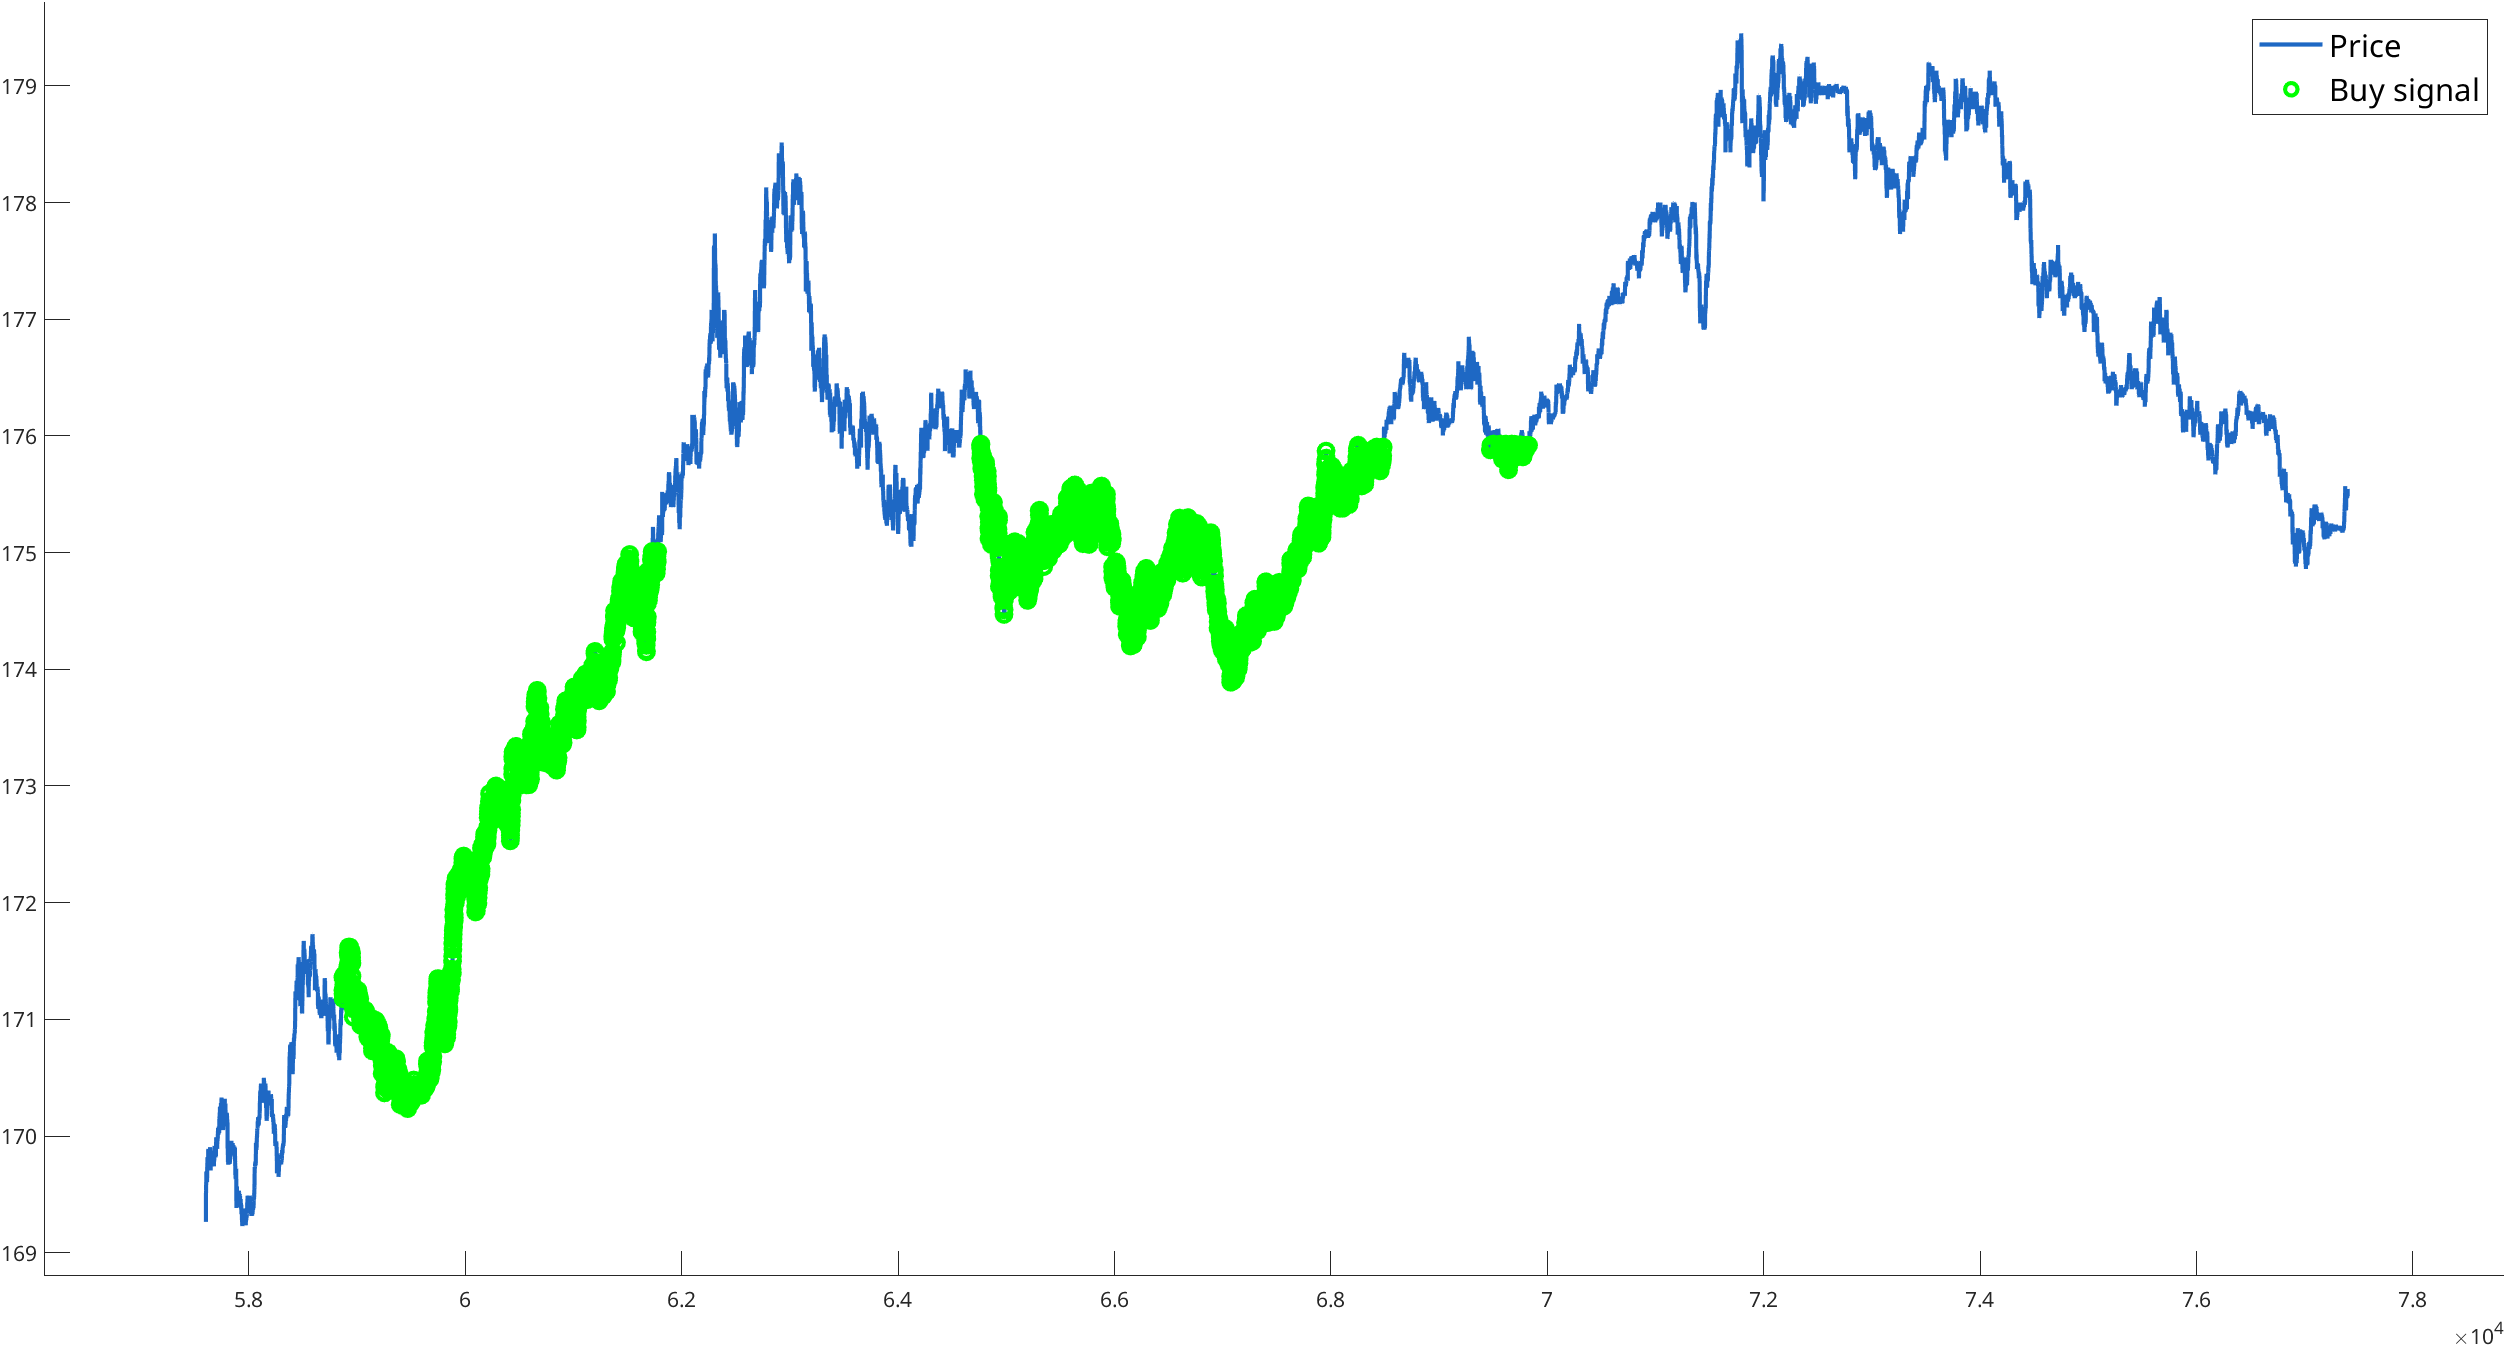
\includegraphics[width=\linewidth]{kep/buy_heavy_event.png}
			\caption{A single market day that generated over 6,000 \textit{Buy} signals.}
			\label{fig:buy_heavy_event}
		\end{center}
		\end{figure}

\section{Conclusions}
	Even though our end model struggles with busy market days, we presented a framework that can be built upon later, as it was typically able to identify clear market trends. However, it had difficulty generalizing in atypical scenarios with concentrated surges of \textit{Buy} signals, likely due to insufficient exposure to diverse \textit{Buy} patterns during training. Despite these challenges, we have many ideas for further development.

	Our reinforcement learning agent only learned to avoid illegal actions, suggesting flaws in the environment's structure. The next step should be a full reconstruction of the environment, explicitly including LOB data instead of derived features like volatility or SMA. Another major change would be extending the trading horizon. Our experience with the classification model showed that short time intervals contain highly noisy price data, while longer intervals and higher price changes reduce noise and help the model learn patterns. Therefore, the trading horizon in reinforcement learning should be much longer than the current 60 seconds.

	With the LOB method, we hoped the model would recognize more meaningful information due to the extended feature set. However, the increased feature dimension made this approach very memory intensive, making it impossible to load the full training set into memory. We tried using MATLAB's datastore objects, which allow handling many files as a single entity during training. The issue was that existing datastores read entire files at once, not in a structured mini-batch format. Saving mini-batches as separate files was also unfeasible due to the large number of mini-batches required. One way to solve this memory issue is by creating a custom datastore that can read data from multiple larger files as mini-batches, eliminating the need to load the full training set into memory.

	To help our model better recognize the currently problematic buy signals, we could include more diverse data in our training set. Currently, technical limitations prevent this. We have to store the raw market data in a local MySQL database on the development machine, which significantly limits accessible information because the original database contains multiple terabytes of data. Unfortunately, due to the development machine's storage capacity, we can only keep a subset locally. With a dedicated server, we could access and process more data, diversify our training set, and potentially improve the performance of our latest model.

	Exploring more complex network architectures could be the next step. Bidirectional LSTMs (BiLSTMs), which process sequences forward and backward to capture context from both past and future, may learn more abstract patterns. Another option is convolutional LSTMs (ConvLSTMs), which combine convolutional neural networks (effective at extracting spatial features) with LSTMs (excel at modeling temporal dependencies). ConvLSTMs can help the model better capture both spatial and temporal patterns, potentially improving prediction accuracy.

\section*{Summary}
In this work we have examined how raw, high-resolution data can be processed and analyzed and how it can be used with machine learning models. The overall goal was to construct a system capable of identifying profitable opportunities. To achieve this, we worked on data processing preprocessing, model design, implementation, training, and evaluation.

First, two methods were implemented to process raw stock market data into formats suitable for machine learning: the tick price method and the limit order book (LOB) method. The tick price method created sequences from timestamped ticks. To address the issue of nonuniform time gaps between ticks, two versions were developed. In the interpolated version, prices were interpolated within fixed trading intervals. In the raw version, original prices were kept, and the time elapsed since the previous tick was added as a feature to account for variable gaps. The LOB method involved fully reconstructing the limit order book from market depth updates. Snapshots of the LOB were taken periodically and formatted for efficient programmatic use. Finally, all data generated by these methods were annotated using a specified price threshold and time interval. The last step of data processing was balancing, to prevent class bias during training.

We created a basic reinforcement learning setup, using the LOB snapshots generated by the LOB method as the foundation of the environment. Observations were defined using data derived from the LOB, and the agent's possible actions and corresponding reward functions were specified. The agent was trained using Deep Q-learning (DQN) with an LSTM based architecture. However, the reinforcement learning approach remained in an early stage due to suboptimal results.

The supervised learning approach involved two network architectures: a LeNet based CNN and an LSTM based RNN. The CNN followed the classic LeNet-5 structure with additional layers added to handle longer input sequences. The LSTM network included two stacked LSTM layers, aiming to improve the model's ability to learn more complex patterns.

In total, over 600 tests were conducted to determine which network architecture performs best under various parameters. We concluded that both the LSTM and LeNet architectures can learn from sequential price data. The LSTM performed better on shorter sequences but its performance declined with longer ones. In contrast, LeNet improved with longer sequences. Since our goal was a long prediction horizon, the LeNet architecture was preferred for further work. Through extensive testing, optimal hyperparameters were identified. These primarily included data processing settings such as the price threshold, future price checking window, price difference margin, sequence length, and whether to interpolate price data.

Based on our experiments, using a larger future price window and targeting greater price increases produced more recognizable patterns. In our case, introducing a margin value to better differentiate the classes decreased the network's performance. The same was observed with price interpolation, as the network performed better when trained on data generated by the raw price method.

In our final testing series, we determined that the model's performance varied significantly depending on the selected days. Accuracy ranged from 50\% to over 95\% across all three stocks tested. Confusion matrices showed that the model performed best on days with few or no \textit{Buy} signals, and worst when the number of \textit{Buy} signals were unusually high. This was likely due to limited diversity in \textit{Buy} samples during training. While the dataset was balanced overall, most \textit{Buy} signals came from a few events, unlike \textit{Hold} samples drawn from many days. This imbalance may negatively affected generalization. However, our proposed model demonstrated its ability to learn meaningful patterns, achieving over 90\% accuracy in some cases. Since the training set was roughly balanced between classes, these results reflect genuine predictive skill rather than class bias. Under the right conditions, the model showed strong performance and clear potential for further refinement and practical use.

\pagebreak
% \sectionimage{kep/header3.png} % Chapter heading image
\section*{Resumé}
\addcontentsline{toc}{chapter}{Resumé}
\markboth{}{\sffamily\normalsize{Resumé}}
Cieľom tejto diplomovej práce je analyzovať údaje z akciového trhu s vysokým rozlíšením a aplikovať neurónové siete na vývoj víťazných obchodných stratégií. Výskum sa zameriava na predpovedanie pohybu cien na akciovom trhu, ktoré sú podmienené dynamikou ponuky a dopytu a sú aktívne skúmanou oblasťou. V práci sa prezentuje vývoj aplikácie, ktorá je schopná predbežne spracovať údaje z akciového trhu v reálnom čase a trénovať neurónové siete. Získané výsledky sa vyhodnotia. Vývoj je rozdelený do dvoch hlavných krokov: predbežné spracovanie údajov a konštrukcia neurónových sietí so zameraním na rekurentné neurónové siete (RNN) založené na dlhej krátkodobej pamäti (LSTM) a konvolučné neurónové siete (CNN) podľa topológie LeNet. Práca pozostáva zo siedmich kapitol, ktoré podrobne opisujú teoretické východiská, metodiku, proces vývoja, výsledky testovania a možnosti ďalšieho rozvoja výskumu.

Prvá kapitola práce sa zaoberá základmi burzy cenných papierov s osobitným zameraním na fungovanie trhu NASDAQ. Predstavuje základné mechanizmy obchodovania s akciami, ako je úloha ponuky a dopytu pri určovaní cien a význam trhových údajov pri algoritmickom obchodovaní. Kapitola stručne rozoberá typy údajov akciového trhu, ako sú údaje level 1 a level 2, ktoré zahŕňajú hĺbku trhu a ceny v reálnom čase. V závere kapitoly je predstavený nástroj na rekonštrukciu knihy hĺbky (LOB) s názvom LOBSTER. Teoretické základy v tejto kapitole poskytujú potrebný kontext pre následnú technickú analýzu.

Druhá kapitola opisuje základy strojového učenia so zameraním na neurónové siete. Preberá základné pojmy strojového učenia, ako sú učenie pod dohľadom, spätné šírenie a algoritmy gradientného zostupu. Osobitná pozornosť bude venovaná fungovaniu sietí LSTM, ktoré sú vďaka svojej schopnosti modelovať dlhodobé závislosti obzvlášť vhodné na analýzu časových radov údajov, ako sú napríklad ceny na burze. Predstavíme aj základy konvolučných neurónových sietí (CNN), pričom zdôrazníme použiteľnosť architektúry LeNet pri rozpoznávaní vzorov. Kapitola sa zaoberá aj výzvami strojového učenia, ako je problém nadmerného prispôsobovania a úloha vypadávajúcich vrstiev pri jeho predchádzaní.
Tretia kapitola predstavuje tri relevantné projekty a štúdie, ktoré sa zameriavajú na vývoj algoritmických obchodných nástrojov. Tieto projekty využívajú rôzne prístupy k analýze údajov z akciového trhu, napríklad modely hlbokého učenia a posilňovanie učenia. Prvým je open-source projekt, ktorý využíva "deep Q-learning" na učenie agenta posilneného učenia, aby robil vhodne načasované rozhodnutia o nákupe a predaji. Údaje sú založené na záverečných cenách akcií. Druhý dokument predstavuje systém založený na posilňovaní učenia, ale podstatne zložitejší.  Systém je založený na tzv. topológii EIIE, kde konečný výstup systému je spriemerovaným výstupom viacerých podsystémov. Prostredie posilneného učenia je založené na kryptotrhu, v rámci ktorého niekoľko architektúr robí trhové rozhodnutia o nákupe a predaji. Medzi testované architektúry patria CNN a RNN. Pri hodnotení získali CNN aj RNN výraznú výhodu oproti svojim konkurentom. A napokon tretí článok opisuje implementáciu systému na predpovedanie cien akcií. Hoci počas testov systém nedokázal presne predpovedať zatváraciu cenu akcií, napriek tomu dokázal určiť trend na trhu. V závere kapitoly zdôrazňujeme, ako výsledky predchádzajúceho výskumu inšpirovali metodiku tejto práce, najmä v oblasti spracovania údajov v reálnom čase a aplikácie neurónových sietí.

Štvrtá kapitola podrobne opisuje ciele a prístup k práci. Cieľom je vytvoriť systém, ktorý sa dokáže naučiť víťazné obchodné stratégie analýzou údajov z akciového trhu s vysokým rozlíšením. Navrhovaný systém dokáže predbežne spracovať údaje z akciového trhu a natrénovať neurónovú sieť a následne vyhodnotiť jej výkonnosť prostredníctvom simulácií.

Piata kapitola opisuje implementáciu programu a proces vývoja. Medzi nástrojmi a rámcami použitými pri vývoji je MATLAB, ktorý poskytuje bohatú a modulárnu sadu nástrojov na efektívnu implementáciu modelov strojového učenia. V tejto kapitole sú uvedené podrobnosti o zbere a predbežnom spracovaní údajov. Zber údajov sa uskutočnil prostredníctvom rozhrania API Interactive Brokers TWS, ktoré umožňuje zber trhových údajov v reálnom čase, ako sú napríklad údaje level 1 (najlepšie nákupné a predajné ceny) a level 2 (hĺbka trhu). Nespracované trhové údaje sa budú zbierať v rámci Univerzity Selyeho Jánosa od roku 2020. Boli implementované dve metódy spracovania údajov: metóda "tick price", ktorá využíva teoretickú cenu akcií, a metóda "LOB", ktorá je založená na rekonštrukcii troch úrovní LOB. Pri oboch metódach boli údaje prevedené na sekvencie, ktoré boli označené ako "Buy" a "Hold" na základe definovaného prahu nárastu ceny a časového intervalu. Metóda tick price má dve verzie: "interpolated" vytvára rovnomerné údajové body každú sekundu interpoláciou, zatiaľ čo "raw" využíva pôvodné ceny a časové rozdiely (delta time). Metóda LOB generuje snímky LOB, ktoré sú formátované podobne ako LOBSTER, s tromi úrovňami hĺbky. Údaje sú vyvážené pomocou vlastnej vyvažovacej funkcie, aby sa znížila disproporcionalita medzi triedami "Hold" a "Buy", pričom testovacie a validačné súbory údajov zostávajú realistické a nevyvážené. Okrem toho v piatej podkapitole podrobne opisujeme aj vytvorenie prostredia a agenta posilneného učenia pomocou nástroja Reinforcement Learning Designer programu MATLAB, ktorý je postavený na rekurentnej neurónovej sieti založenej na Deep Q-learningu (DQN) s 256 neurónovými vrstvami LSTM. Prostredie využíva vopred spracované údaje LOB, pričom sa v danom čase zameriava len na jednu akciu. Epizódy sa začínajú s pevným rozpočtom a nulovou držbou, pričom 60-sekundový obchodný horizont obmedzuje čas držby akcií. V každom časovom okamihu agent dostáva pozorovania, ktoré zahŕňajú trhové podmienky (krátkodobé cenové trendy, jednoduchý kĺzavý priemer, rovnováhu veľkosti ponuky a dopytu, rozpätie, volatilitu) a jeho vlastnú finančnú situáciu (hotovosť, počet akcií, hodnotu portfólia, zostávajúci čas). Agent si môže vybrať medzi tromi akciami: "Buy" (kúpiť akcie za najlepšiu predajnú cenu s použitím všetkej hotovosti), "Sell" (predať všetky akcie za najlepšiu nákupnú cenu) alebo "Hold" (pasívny stav). Funkcia odmeňovania je zameraná na ziskovosť: fixná pokuta za neplatné akcie, odmena vypočítaná na základe zisku alebo straty za platné akcie, zatiaľ čo akcia "Hold" penalizuje dlhé držanie a pasivitu počas volatilného obdobia. Epizóda sa končí, keď agent dosiahne posledný časový bod alebo mu dôjdu peniaze a nedrží žiadne akcie. V poslednej podkapitole kapitoly 5 podrobne opisujeme štruktúru klasifikačných modelov. Na učenie pod dohľadom sme testovali dva modely: rekurentnú neurónovú sieť (RNN) založenú na LSTM a konvolučnú neurónovú sieť (CNN) podľa topológie LeNet. Model LSTM pozostáva z dvoch vrstiev, prvej s 256 neurónmi a druhej so 128 neurónmi, pričom prvá vrstva vracia sekvenciu a druhá vracia jednu značku. Za oboma vrstvami bola použitá dropout vrstva s 25\%, aby sa znížilo nadmerné prispôsobovanie. V prípade dlhých sekvencií je CNN založená na sieti LeNet rozšírená o dodatočnú konvolučnú vrstvu-ReLU-max pooling a obsahuje dve hlavné sady konvolučných vrstiev (6 a 16 filtrov, veľkosť jadra $1\times5$ a $1\times11$, dĺžka kroku 5 a 16). Na zachovanie veľkosti výstupu sme použili "rovnaké" vypĺňanie pre dvojicu konvolučných vrstiev. Vrstvy s maximálnym združovaním sa zmenšili na veľkosť fondu 2, po ktorých nasledujú tri "plne pripojené" vrstvy. Pre model LSTM sme ako vstup použili "sequenceInputLayer", zatiaľ čo pre CNN sme použili jedinečnú vstupnú vrstvu, pričom sme definovali vstupný formát ako "BTC" (batch-time-channel), aby sme zabezpečili správnu interpretáciu sekvencií a deskriptorov. Oba modely končia "plne prepojenou" vrstvou s počtom neurónov rovnajúcim sa počtu tried.

Šiesta kapitola opisuje testovanie a hodnotenie dokončených systémov. Prvá podkapitola sa zaoberá testovaním a vyhodnotením implementácie posilneného učenia. Počas testovania sme nastavili rôzne parametre prostredia (počiatočný kapitál, faktor škálovania odmeny, veľkosť okna SMA a volatility) a parametre učenia (rýchlosť učenia, veľkosť dávky, epsilon skúmania, rýchlosť znižovania učenia a skúmania, počet epoch), pričom optimálne hodnoty sme hľadali metódou pokusov a omylov. Na základe výsledkov testov sa agent nedokázal naučiť žiadne zmysluplné vzory a zdalo sa, že si vyberá náhodne z troch obchodných akcií. Hoci sa agent naučil vyhýbať sa neplatným akciám, zmena parametrov nezlepšila výkonnosť, takže sme problém pripísali štruktúre procesu učenia a prostredia. Namiesto prepracovania prostredia na učenie posilňovaním sme sa zamerali na prístup učenia s učiteľom založený na skúsenostiach s dlhším horizontom predpovedania viac ako 60 sekúnd, aby sme znížili šum a pomohli odhaliť významnejšie vzory. V druhej podkapitole kapitoly 6 sa zaoberáme porovnaním neurónových sietí založených na LSTM a LeNet, výkonnosťou metód spracovania cien LOB a tick a hľadaním optimálnych parametrov. Testované parametre spracovania údajov zahŕňajú interpoláciu cien, prah prírastku cien, veľkosť rezervy medzi dvoma triedami, časové okno na kontrolu budúcich cien a dĺžku sekvencie, pričom z parametrov učenia sa menila len veľkosť minibatchu. Modely sa trénovali na údajoch o akciách Disney s optimalizátorom Adam (miera učenia 0,001), maximálne do 1000 epoch, s validačnou toleranciou 20 a funkciou straty cross-entropy. Pri testoch sa kvôli porovnateľnosti použili identické súbory údajov a parametre, pričom pre každú kombináciu parametrov sa vykonali aspoň tri testy. Výsledky ukazujú, že LSTM dosahuje lepšie výsledky pri vyšších prahových hodnotách cenovej odchýlky (napr. 1,5\% alebo 2\%), zatiaľ čo LeNet dosahuje lepšie výsledky pri dlhších sekvenciách a nižších prahových hodnotách, hoci výkonnosť LSTM sa pri dlhších sekvenciách zhoršuje, pravdepodobne v dôsledku problému miznúceho gradientu. Skúmali sme aj vplyv parametrov spracovania údajov: menšie prahové hodnoty a dlhšie časové okná zväčšujú veľkosť súboru údajov, ale vnášajú šum, zatiaľ čo väčšie prahové hodnoty a kratšie časové okná vedú k menšiemu počtu, ale čistejším údajom. Ďalšie testy sa zamerali na sieť LeNet s prahovými hodnotami cenových zmien 1,5\% alebo vyššími a dlhšími sekvenciami, aby sa zabezpečilo, že model lepšie zachytí vzory pred výraznými cenovými zmenami. V pokračovaní tejto podkapitoly je podrobne opísané testovanie časových okien, dĺžok sekvencií a prahov cenových zmien a porovnanie metód spracovania údajov. Testy sa vykonávajú s použitím 184 dní údajov, "raw" metódy tick price, rozpätia cenových zmien 0,5\% a veľkosti minisérie 32 768. Cieľom bolo určiť optimálny prah zmeny ceny (\texttt{price\_diff\_threshold}), okno kontroly budúcej ceny (\texttt{future\_price\_check}) a dĺžku sekvencie (\texttt{sequence\_length}). Výsledky ukázali, že pri prahu 2,5\% a dlhších sekvenciách (napr. 1 500) sa dosiahla až 98,05\% presnosť, ale výsledkom bol menší súbor údajov (~ 11 000 vzoriek), čo zvýšilo riziko nadmerného prispôsobenia. Dlhšie časové okná (7 200 s) zväčšili veľkosť súboru údajov, ale znížili presnosť v dôsledku hlučnejších vzoriek. Vyvážená konfigurácia (prah 2\%, dĺžka sekvencie 1 200, časové okno 7 200 s) dosiahla 92,51\% presnosť so 72 880 vzorkami, čo ponúka dobrý kompromis medzi výkonom a zovšeobecnením. Potom sa porovnali "raw" a "interpolated" verzie metódy tick price a výkonnejšia verzia sa porovnáva s metódou LOB. Metóda "raw" tick price dosahovala konzistentne lepšiu presnosť ako "interpolated" verzia, zrejme zachovanie pôvodných cien a delta času pomohlo rozpoznávaniu vzoriek. Metóda LOB používa 13 príznakov na jeden časový bod (ceny, veľkosti, delta čas), čo výrazne zvýšilo spotrebu pamäte a čas učenia, čo neumožnilo spravodlivé porovnanie oboch metód. Vzhľadom na sľubné výsledky metódy "surových" cien tikov sme však s ňou pokračovali v ďalších testoch. V ďalšej fáze testovacej sekvencie sa analyzoval vplyv \texttt{price\_diff\_margin} so 184 dňami údajov, dĺžkou sekvencie 1 200 a metódou "raw" tick price. Výsledky testov ukazujú, že zavedenie marže má tendenciu znižovať presnosť modelu, pretože eliminácia nárazníkovej zóny medzi dvoma triedami ponecháva v tréningu menšiu rezervu, čo sťažuje detekciu takýchto modelov. Po definovaní optimálnych parametrov uvádzame testy s modelom natrénovaným s optimálnou konfiguráciou na troch akciách (DIS, BA, FOXA), pričom na testovanie sme vybrali rôzne dni. Presnosť sa výrazne líšila (od 50\% do 95\%+), pričom najlepšie výsledky boli 98,37\% pre DIS, 92,36\% pre BA a 97,01\% pre FOXA. Analýza matíc zámien naznačuje, že model funguje dobre, keď je v daný deň málo alebo žiadne triedy "Buy". Výkonnosť sa výrazne zhoršuje, keď sa v jeden trhový deň koncentruje veľa tried "Buy". Vysvetlenie je pravdepodobne spôsobené nedostatočnou diverzitou triedy "Buy" v trénovacej množine. Hoci je učiaca množina vyvážená medzi značkami "Buy" a "Hold", vzorky "Hold" pochádzajú z viacerých dní (každý z nich drží pevne stanovené množstvo a zároveň sa vyvažujú), zatiaľ čo väčšina signálov "Buy" môže pochádzať len z niekoľkých trhových dní.

Na záver siedmej kapitoly sú zhrnuté výsledky výskumu a navrhnuté ďalšie smery na zlepšenie. Konečný model je schopný identifikovať čisté trhové trendy, ale má problémy v atypických dňoch s koncentrovanými signálmi "Buy", pravdepodobne v dôsledku obmedzenej variability triedy "Buy" v súbore trénovaných údajov. Agent posilneného učenia sa naučil iba vyhýbať sa neplatným akciám, čo naznačuje nedostatky v štruktúre prostredia. Odporúča sa kompletné prepracovanie prostredia, priame používanie údajov LOB namiesto odvodených funkcií (napr. volatility, SMA) a výrazné predĺženie 60-sekundového obchodného horizontu, pretože dlhšie časové intervaly znižujú šum a pomáhajú učiť sa vzory. Pamäťové požiadavky metódy LOB bránili načítaniu celého súboru údajov; MATLAB datastores nepodporovali štruktúrované minidávkové čítanie, preto bol navrhnutý vývoj vlastného datastore-u, ktorý by umožnil minidávkové čítanie väčších dátových súborov. Na zlepšenie rozpoznávania signálov "kúpy" modelu je potrebný rozmanitejší súbor trénovaných údajov, čomu v súčasnosti bráni kapacita používaného počítača, keďže údaje sú v súčasnosti uložené lokálne. Vyhradený server by umožnil prístup k väčšiemu množstvu údajov, čím by sa zlepšila výkonnosť modelu. Ako ďalšia možnosť vývoja sa navrhujú zložitejšie sieťové architektúry, ako napríklad obojsmerné LSTM (BiLSTM) alebo konvolučné LSTM (ConvLSTM), ktoré by mohli lepšie zachytiť priestorové a časové vzory, a tým zvýšiť presnosť predpovede.
\pagebreak

\begingroup
\renewcommand{\cleardoublepage}{}
\renewcommand{\clearpage}{}
\renewcommand{\pagebreak}{}
\printbibliography[title=References]
\addcontentsline{toc}{chapter}{References}
\section*{Attachments}
\begin{figure}[H]
\begin{center}
	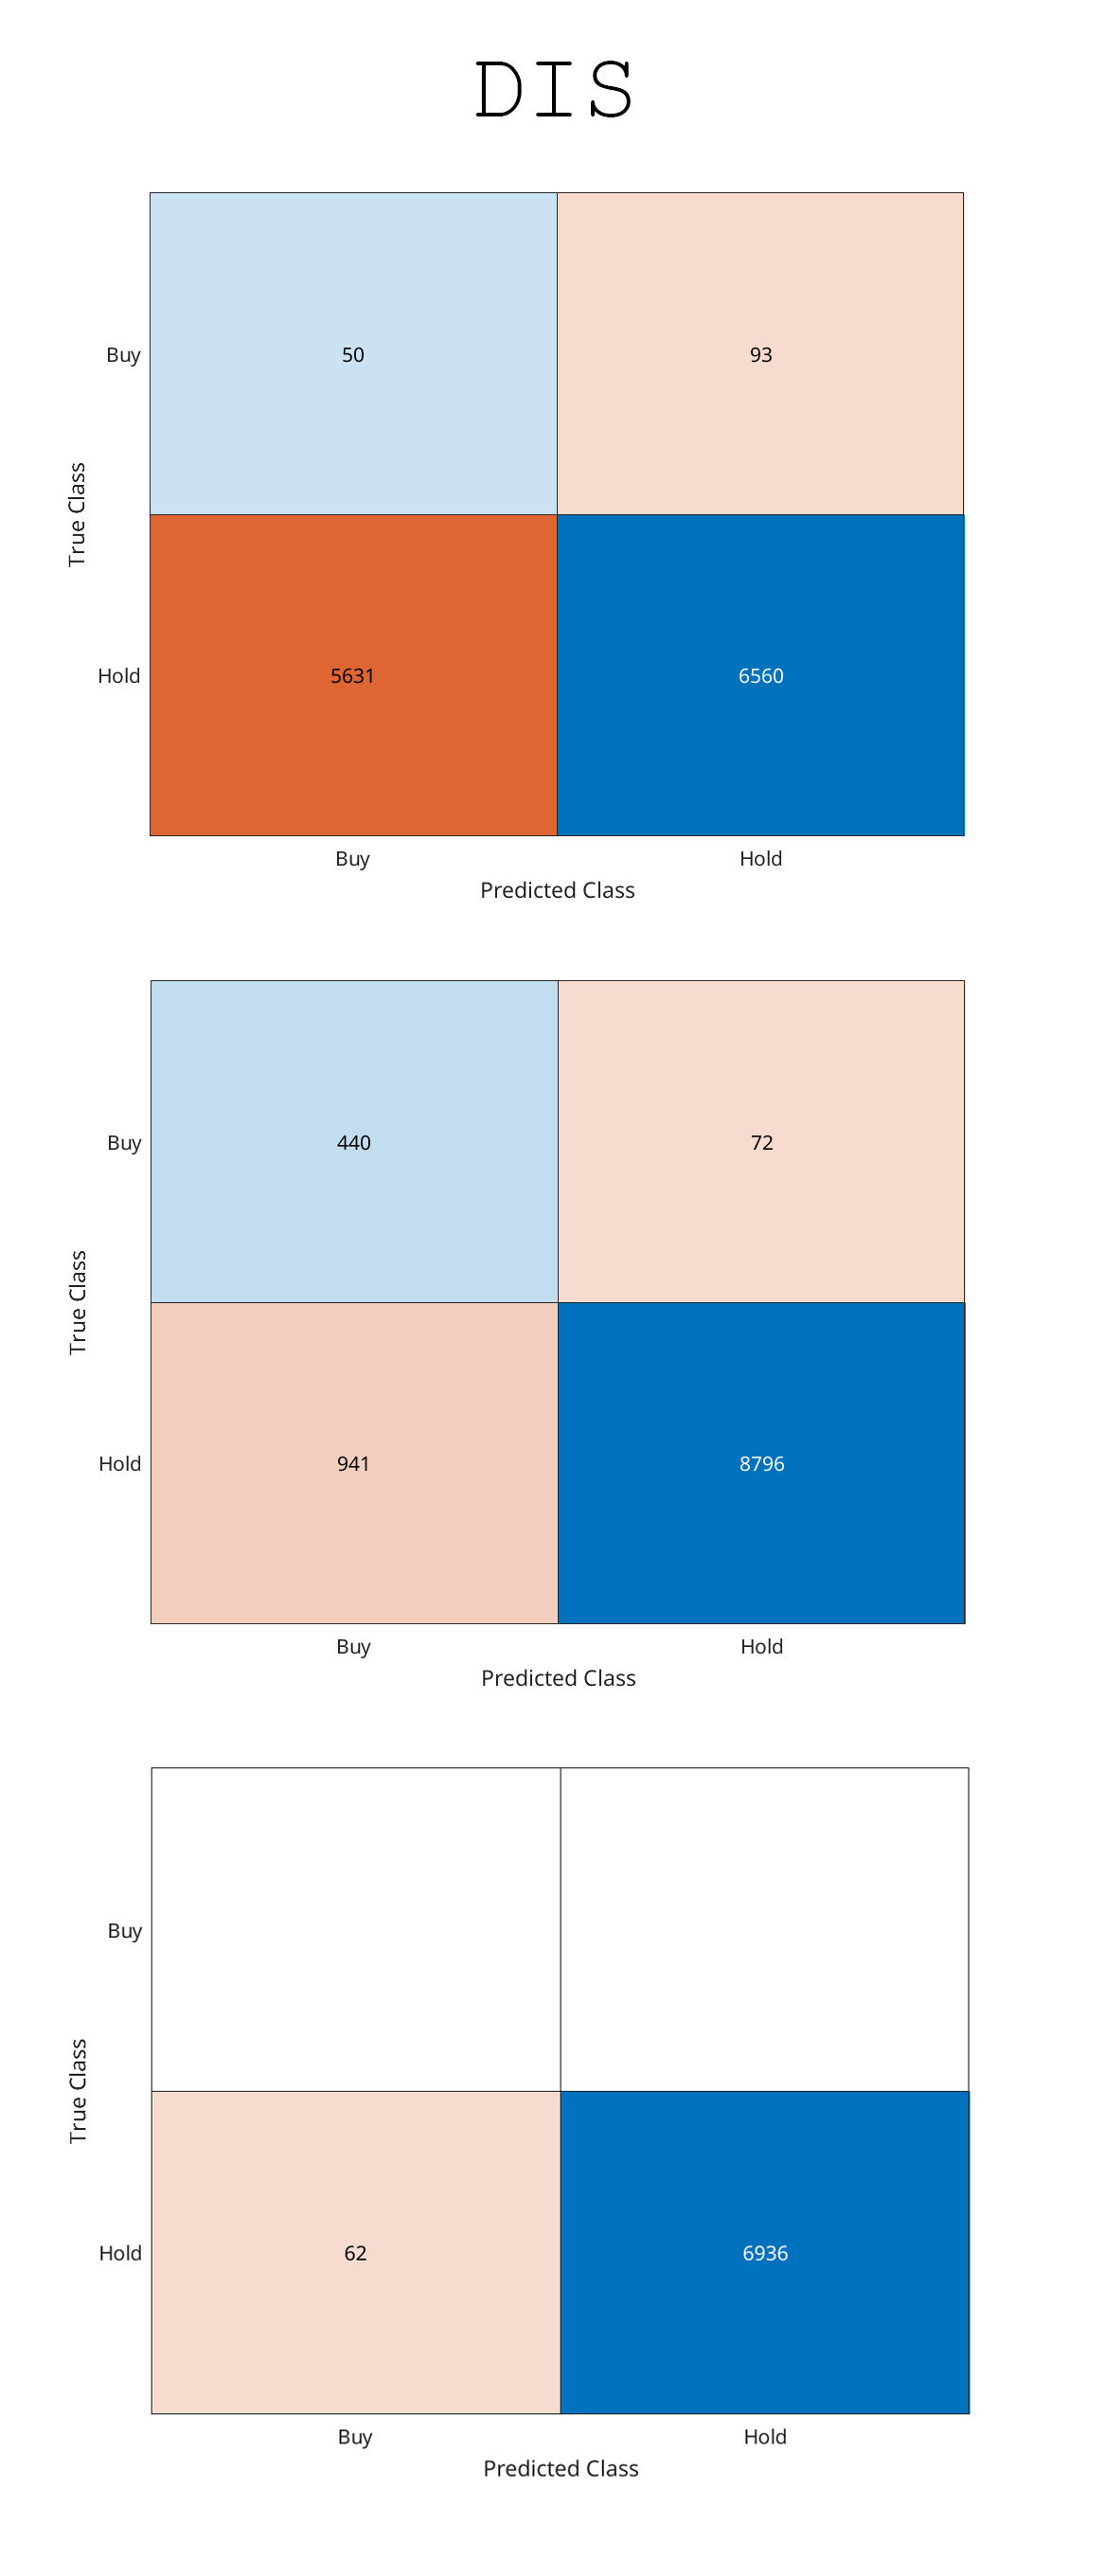
\includegraphics[height=0.8\textheight, keepaspectratio]{kep/DIS2.png}
\end{center}
\end{figure}
\begin{figure}[H]
\begin{center}
	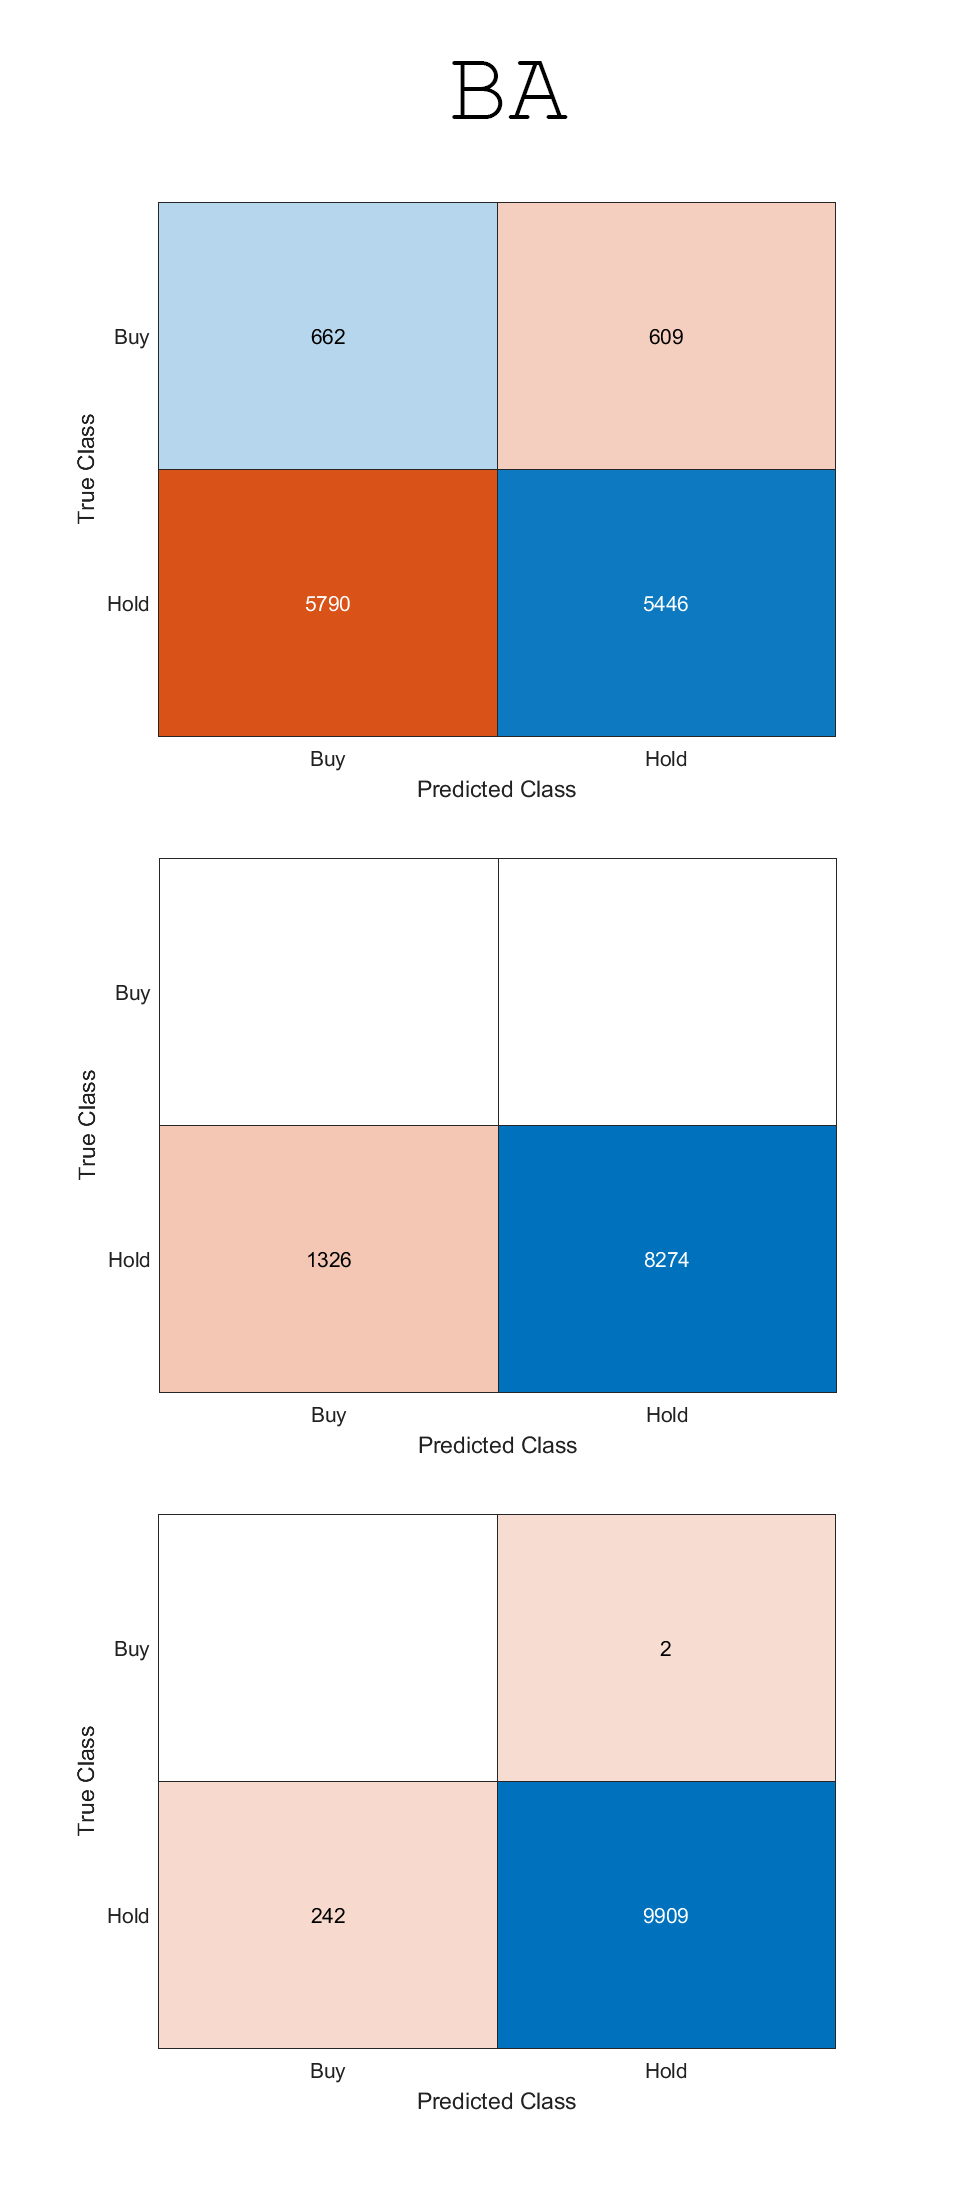
\includegraphics[height=0.8\textheight, keepaspectratio]{kep/BA2.png}
\end{center}
\end{figure}
\begin{figure}[H]
\begin{center}
	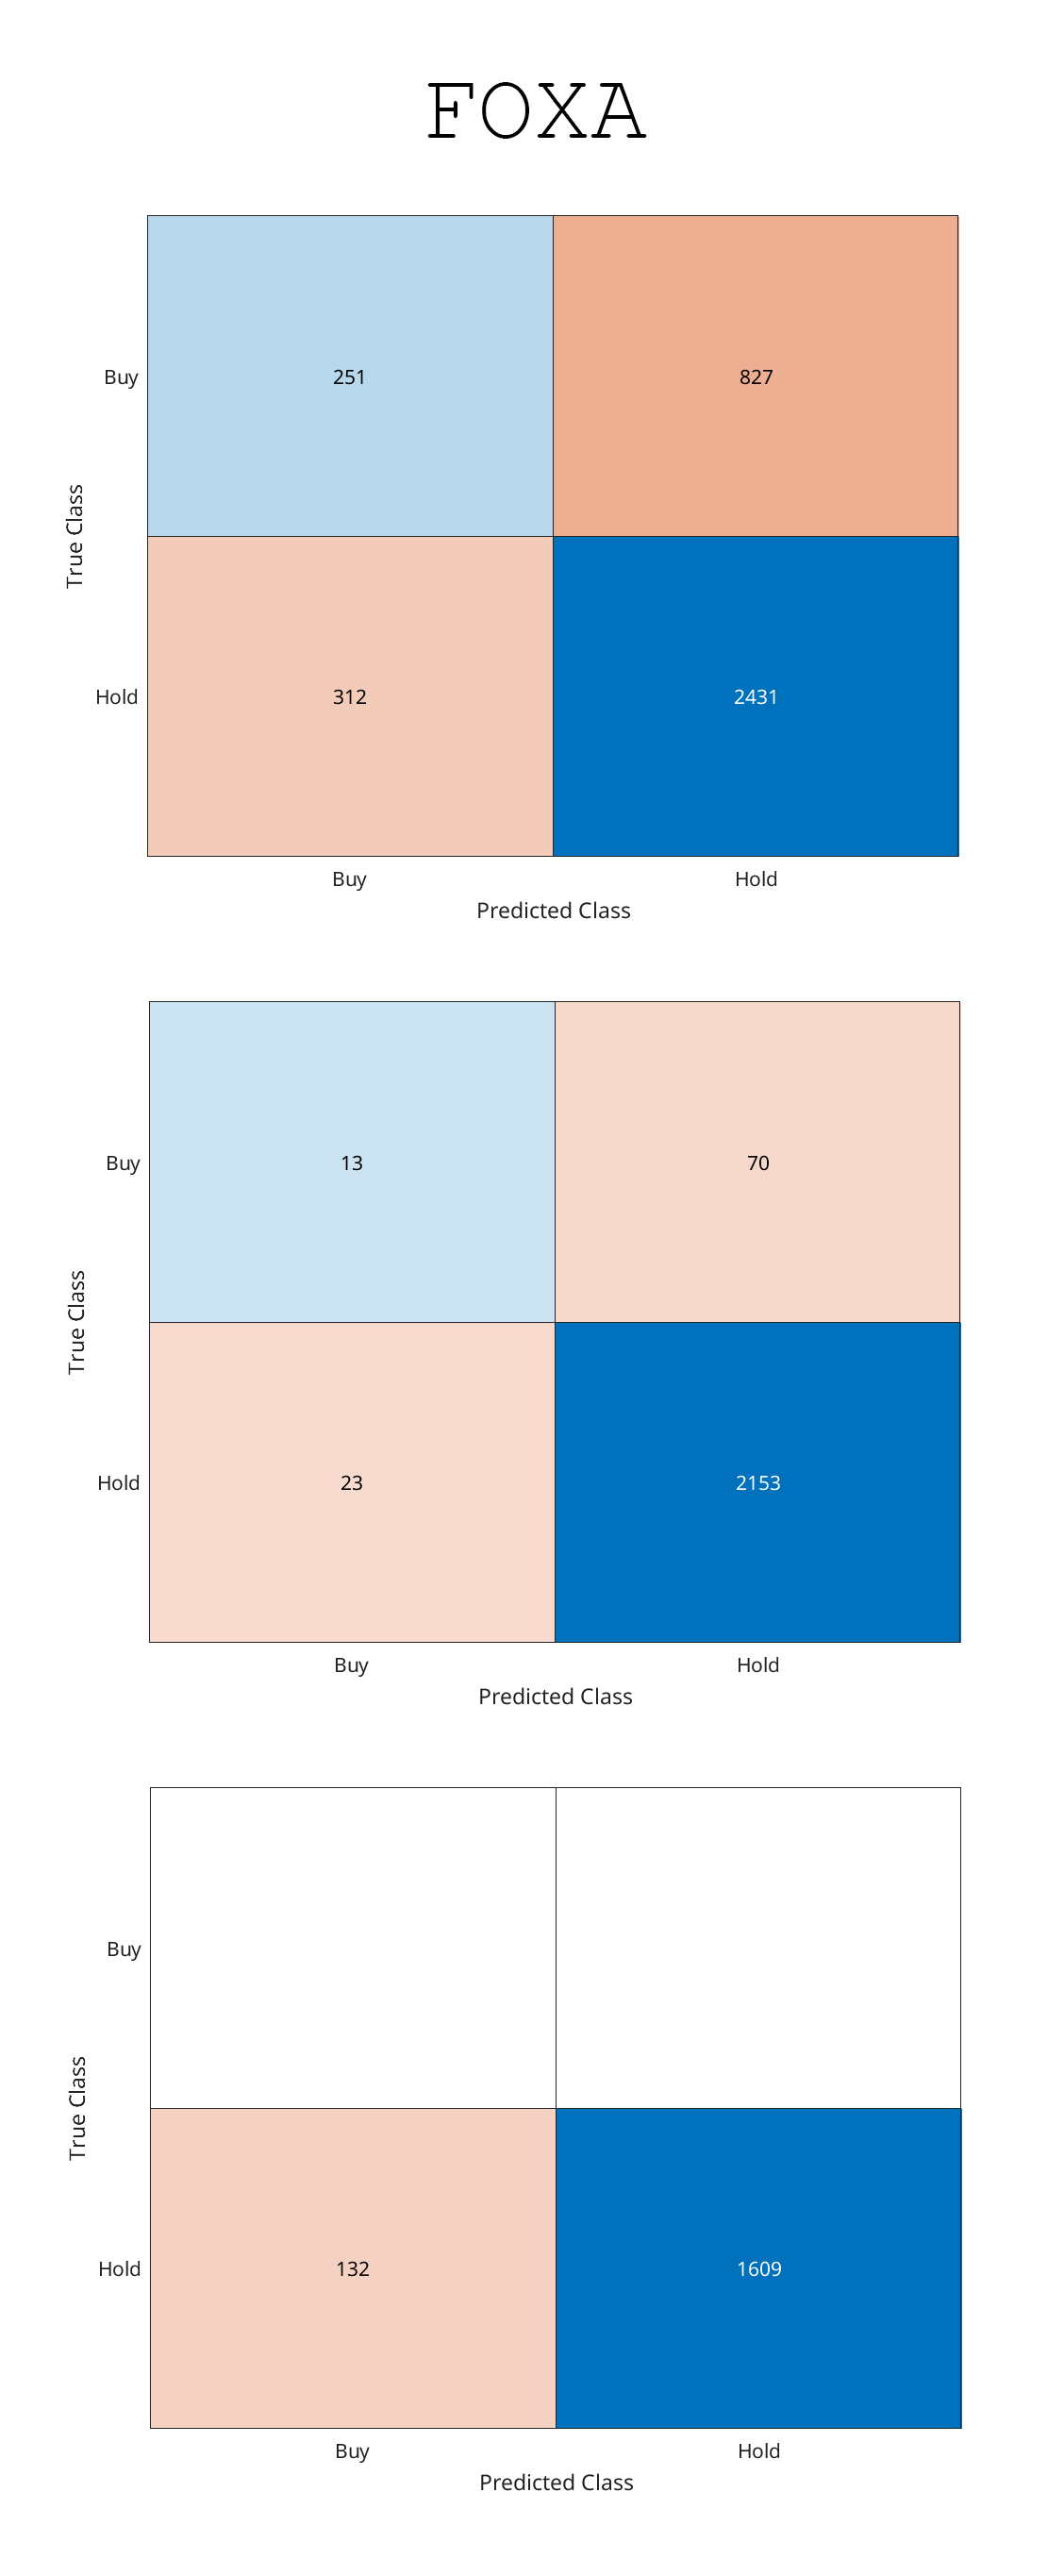
\includegraphics[height=0.8\textheight, keepaspectratio]{kep/FOXA2.png}
\end{center}
\end{figure}
\endgroup

The attached CD contains the source code for the program.

\end{document}
